\documentclass[xcolor={usenames,dvipsnames}
    ,handout
]{beamer}

%
% ugly hack referring to the slides folder. Works for me.
%
\makeatletter
\def\input@path{{/Users/denilson/teaching/cmput391/git-slides/}}
\makeatother

% \usepackage[T1]{fontenc} % font encoding
% \usepackage{fontspec}
\usepackage{fontspec}


\makeatletter%
\@ifclassloaded{beamer}{%
  \usepackage{lmodern} %%% modern beamer style
  %%beamer style
  \usetheme{metropolis}
  \usefonttheme{professionalfonts}
  \setbeamercolor{background canvas}{bg=background}
  \setbeamercolor{frametitle}{bg=snow,fg=black}
  \setbeamercolor{title separator}{fg=snow}
  \setbeamercolor{alerted text}{fg=accent}

  \let\oldtitle\title
  \renewcommand{\title}[1]{\oldtitle{CMPUT391\\#1}}
  \author{Instructor: Denilson Barbosa}
  \date{\small University of Alberta}
  \institute{\today\vskip4em Slides by D. Barbosa, with suggested corrections and improvements by (in alphabetical order) C. Bins, D. Caminhas, K. Guhzva, Q. Lautischer, E. Macdonald, M. A. Nascimento, K. Newbury, M. Strobl, D. Sunderman, K. Wang, and K. Wong.}
  
  \titlegraphic{
\includegraphics[width=1.5cm]{../images/by-sa.png}~
  {\tiny This work is licensed under a Creative Commons Attribution 4.0 International License}}

  %%%% un-framed blocks
  \setbeamertemplate{blocks}[rounded][shadow=false]
}{}

\@ifpackageloaded{xcolor}{}{
  \usepackage{xcolor}
}
\makeatother

\setsansfont[BoldFont={Open Sans SemiBold}]{Open Sans}[Scale=0.9]
\setmonofont{Cousine}[Scale=0.875]
% \setmathtt{Cousine}[Scale=0.875]

%%%% highlighting text 
\usepackage{xspace}
\def\highlight#1{\colorbox{accent}{\textcolor{white}{#1}}\xspace}

\def\blue#1{\textcolor{blue}{#1}}

%
%
%
\usepackage{parskip}

\usepackage{subcaption} % needed for subfigures

\usepackage{wrapfig} % for figures "to the side of the text"

\usepackage{anyfontsize} % for egregious warnings

%
% Fonts
%
% \usepackage{amsmath}
% \usepackage{mathspec}
% \setmathtt[Scale=0.875]{Cousine}

%
% various packages for tables and colored tables
%
\usepackage{xcolor,colortbl}
\usepackage{tcolorbox}

\definecolor{accent}{RGB}{225,68,85}
\definecolor{highlight}{RGB}{170,68,153}
\definecolor{background}{rgb}{253,252,252}

\definecolor{sqlColor}{RGB}{119,119,17}

\definecolor{Cfunction}{RGB}{51,51,153}

\definecolor{stringColor}{RGB}{51,51,153}
\definecolor{datatypeColor}{RGB}{170,68,153}
\definecolor{functionColor}{RGB}{51,134,116}

\definecolor{exampleColor}{RGB}{51,34,136}
\definecolor{commentColor}{RGB}{112,68,225}

\definecolor{fern}{RGB}{80,118,66}

\definecolor{snow}{RGB}{240,240,230}
\definecolor{Gray}{gray}{0.85}

\definecolor{tupleBoxColor}{gray}{0.85}

\definecolor{Maroon}{RGB}{139,0,0}

%
% coloring of SQL code
%
\def\ColorSymbol#1{\textcolor{functionColor}{#1}}

%
% hihglight box
%
\usepackage{xspace}
\def\highlight#1{\colorbox{accent}{\textcolor{white}{#1}}\xspace}

%
% Tables
%
\usepackage{multirow}
\usepackage{multicol}

%
% CODE LISTINGS
%
\usepackage{listings}

%
% catch-all style meant to provide a clean and "empty" style
% from which all others build upon
%
\lstdefinestyle{cmput391}{
  style=,
  frame=no,
  tabsize=2,
  numbers=none,
  showstringspaces=false,
  numberstyle=\footnotesize,
  basicstyle=\ttfamily\footnotesize\color{black},
  numbersep=4pt,
  keywords=[1]{},
  keywords=[2]{},
  keywords=[3]{sh_lock,xl_lock,unlock,read,write,commit,abort},
  keywordstyle=[1]\ttfamily\bfseries\footnotesize,
  keywordstyle=[2]\ttfamily\footnotesize,
  keywordstyle=[3]\ttfamily\footnotesize\color{Maroon},
  emph=[1]{},
  emph=[2]{},
  emph=[3]{},
  emphstyle=[1]\ttfamily\footnotesize,
  emphstyle=[2]\ttfamily\footnotesize,
  emphstyle=[3]\ttfamily\footnotesize,
  commentstyle=\ttfamily\itshape\color{commentColor},
  stringstyle=\ttfamily\color{stringColor},
  moredelim=**[l][\itshape\color{commentColor}]{--},
  moredelim=**[is][\color{highlight}]{-|}{|-},
  moredelim=[is][\bfseries\color{highlight}]{-:}{:-},
  morestring=[s][\color{stringColor}]{"}{"},
  morecomment=[l]{--}
}

\lstdefinelanguage{DTD}{
  style=cmput391,
  morekeywords=[1]{DOCTYPE,ELEMENT,ATTLIST},
  keywordstyle=[1]\color{accent},
  literate = {\#PCDATA}{{\textcolor{Cfunction}{\#PCDATA}}}7
             {\#IMPLIED}{{\textcolor{Cfunction}{\#IMPLIED}}}8
}

\lstdefinelanguage{XPath}{
  style=cmput391,
  morekeywords={xs,integer,current,date,distinct,values,avg,text,id,count,position,and,or,not,boolean,number,sum,floor,ceiling,round,doc,eq,ne,gt,lt,ge,le},
  keywordstyle=\color{red},
  literate = {last(}{{\textcolor{functionColor}{last}(}}5 {@<}{{<}}1  
}

\lstdefinestyle{XQuery}{
  style=cmput391,
  keywords=[1]{if,then,else,and,or,some,every,satisfies,for,in,let,where,group,order,by,return,ascending},
  keywords=[2]{gt,lt,eq,ne,ge,le,not,or},
  keywords=[3]{text,sum,min,max,avg,len,position,number,boolean,floor,ceiling,round,%
               id,doc,count,current-date,distinct-values,xs:integer,subsequence},
  keywordstyle=[1]\bfseries\color{sqlColor},
  keywordstyle=[2]\color{accent},
  keywordstyle=[3]\color{functionColor},
  moredelim =[is][\color{blue}]{-:}{:-},
  moredelim =[s][\color{accent}]{<}{>},
  moredelim=**[s][\color{black}]{/}{\ },
  moredelim=*[s][\color{blue}]{\$}{\ },
  alsoletter=:{:,-},
  literate = {(}{{\textcolor{black}{(}}}{1} {)}{{\textcolor{black}{)}}}{1} 
             {\{}{{\textcolor{black}{\{}}}{1} {\}}{{\textcolor{black}{\}}}}{1} 
             {last(}{{\textcolor{functionColor}{last}(}}5 {@<}{{<}}1
}


\lstdefinestyle{SQL}{
  style=cmput391,
  language=SQL,
  sensitive={True},
  deletekeywords={year,Cast,MIN,MAX},
  morekeywords={ABORT,AFTER,BEFORE,REFERENCES,REFERENCING,WITH,COMMITTED,UNCOMMITTED,REPEATABLE,SERIALIZABLE},
  keywords=[2]{AVG,MIN,MAX,COUNT,SUM,NEW,OLD,strftime,date,length,RAISE,rowid,substr},
  keywords=[3]{BIGINT,CHAR,DATE,DECIMAL,INT,FLOAT,TEXT},
  keywordstyle=[1]\ttfamily\bfseries\color{sqlColor},
  keywordstyle=[2]\ttfamily\bfseries\color{functionColor},
  keywordstyle=[3]\ttfamily\bfseries\color{datatypeColor},
  moredelim=**[is][\ttfamily\bfseries\color{functionColor}]{(@}{@)},
  morestring=[s][\color{stringColor}]{'}{'},
  moredelim=[is][\bfseries\color{highlight}]{-:}{:-}
}


%
% lstlisting for command line examples
%
\lstdefinestyle{commandLine}{
  basicstyle=cmput391,
  keywordstyle=[1]\ttfamily\bfseries\color{functionColor},
  keywordstyle=[2]\ttfamily\bfseries\color{datatypeColor},
  moredelim=**[is][\color{accent}\bf]{@}{@}
  keywords=[1]{%
    grep},
  keywords=[2]{%
    postings}
}

%
% lstlisting for C code
%
\lstdefinestyle{C}{
  language=C,
  tabsize=2,
  basicstyle=\ttfamily\footnotesize,
  stringstyle=\color{stringColor},
  keywords=[2]{sqlite3_prepare_v2,sqlite3_bind_int64,sqlite3_step,sqlite3_exec},
  keywordstyle=[1]\ttfamily\bfseries\color{datatypeColor},
  keywordstyle=[2]\ttfamily\bfseries\color{functionColor},
  commentstyle=\ttfamily\itshape\color{commentColor},
  moredelim=**[is][\color{Cfunction}\bf\ttfamily]{@}{@}
}


\lstdefinestyle{Python}{
  language=Python,
  tabsize=2,
  basicstyle=\ttfamily\footnotesize,
  stringstyle=\color{stringColor},
  morekeywords=[1]{self,yield,Class,true,false,None},
  keywords=[2]{satisfies,from,Iterator,EOF,concatenate,advance,join,rewind},
  deletekeywords=[1]{from},
  keywordstyle=[1]\ttfamily\bfseries\color{datatypeColor},
  keywordstyle=[2]\ttfamily\bfseries\color{functionColor},
  commentstyle=\ttfamily\itshape\color{commentColor},
  moredelim=**[is][\color{Cfunction}\bf\ttfamily]{@}{@}
}



%
% lstlisting style for RDF/SPARQL
%
\lstdefinestyle{SPARQL}{
  style=cmput391,
  sensitive={True},
  keywords=[1]{BASE,PREFIX,SELECT,WHERE,FILTER,MINUS,NOT,EXISTS},
  keywordstyle=[1]\ttfamily\bfseries\color{sqlColor},
  moredelim=*[s][\color{Cfunction}]{?}{\ },
  moredelim=*[s][\color{Cfunction}]{@}{\ },
  morestring=[s][\color{datatypeColor}]{"}{"},
  literate =* {|}{{|}}1 {//}{{//}}2 {< }{< }{2}
}

%
% coloring of markup code
%
\lstdefinestyle{markup}{
  style=cmput391,
  literate =* {=}{{\color{sqlColor}{=}}}1,
  moredelim =* [s][\color{accent}]{<}{>},
  moredelim =** [is][\color{accent}]{@}{@},
  moredelim =** [is][\color{blue}]{-:}{:-},
  morecomment=[s]{<!--}{-->}
}

\lstdefinestyle{RDF}{
  style=cmput391,
  keywords=[1]{BASE,PREFIX},
  keywordstyle=[1]\ttfamily\bfseries\color{functionColor},
  alsoletter=:{:,-,@},
  literate = {prefix}{{\bfseries\textcolor{functionColor}{prefix}}}6 
             {:}{{\textcolor{functionColor}{:}}}1 
             {@}{{\textcolor{functionColor}{@}}}1,
  moredelim =* [s][\color{accent}]{<}{>},
  moredelim =** [is][\color{functionColor}]{-:}{:-},
  morecomment=[s]{<!--}{-->}
}




















%
% Tikz stuff, for cummulative diagrams and algebra trees
%
\usepackage{tikz} %commutative diagrams
\usepackage{tikz-cd} %commutative diagrams
\usetikzlibrary{positioning}% To get more advances positioning options
\usetikzlibrary{arrows,shapes,automata}
\usetikzlibrary{calc} % for calculations and hard-coded coordinates
\usetikzlibrary{tikzmark, fit, shapes.misc}
\usetikzlibrary{decorations.pathreplacing}
\usetikzlibrary{backgrounds} % to draw underneath other elements
\usepackage{stackengine} % to overlay tikz pictures over other things

\usepackage{pgfplots}
\pgfplotsset{compat=1.17}

%
%
% PGF arrowtip that looks like an X
%
%
\pgfarrowsdeclare{X}{X}
{
  \arrowsize=0.25pt
  \advance\arrowsize by .5\pgflinewidth
  \pgfarrowsleftextend{-4\arrowsize-.5\pgflinewidth}
  \pgfarrowsrightextend{.5\pgflinewidth}
}
{
  \arrowsize=0.2pt
  \advance\arrowsize by .5\pgflinewidth
  \pgfsetdash{}{0pt} % do not dash
  \pgfsetroundjoin   % fix join
  \pgfsetroundcap    % fix cap
  \pgfpathmoveto{\pgfpointorigin}
  \pgfpathlineto{\pgfpoint{-5\arrowsize}{5\arrowsize}}
  \pgfusepathqstroke
  \pgfpathmoveto{\pgfpointorigin}
  \pgfpathlineto{\pgfpoint{5\arrowsize}{-5\arrowsize}}
  \pgfusepathqstroke
  \pgfpathmoveto{\pgfpointorigin}
  \pgfpathlineto{\pgfpoint{-5\arrowsize}{-5\arrowsize}}
  \pgfusepathqstroke
  \pgfpathmoveto{\pgfpointorigin}
  \pgfpathlineto{\pgfpoint{5\arrowsize}{5\arrowsize}}
  \pgfusepathqstroke
}


%
%%% for algorithms and pseudocode
%
\usepackage{algorithm}
% \usepackage{algpseudocode}
\usepackage[noend]{algpseudocode}
\renewcommand{\algorithmicrequire}{\textbf{Input:}}
\renewcommand{\algorithmicensure}{\textbf{Output:}}
\algnewcommand\algorithmicforeach{\textbf{for each}}
\algdef{S}[FOR]{ForEach}[1]{\algorithmicforeach\ #1\ \algorithmicdo}
% style for comments inside algorithms
\renewcommand{\algorithmiccomment}[1]{\hspace*{1em}\textcolor{commentColor}{\%~\textit{#1}}} 

%
% to create boxes with verbatim and code-like content
%
\usepackage{verbatimbox}

%
% to crop/trim boxes!
%
\usepackage{trimclip}

%
% colored and framed boxes
%
\newenvironment{BOX}[1]{\begin{tcolorbox}[colback=snow!25,colframe=snow!40!black,title=#1]\small}{\end{tcolorbox}}



%
% math and symbols
%
\usepackage{mathtools}
\DeclarePairedDelimiter{\ceil}{\lceil}{\rceil}
\DeclarePairedDelimiter{\floor}{\lfloor}{\rfloor}
\usepackage{amsbsy} 
\usepackage{amssymb}
\usepackage{ifsym} % needed to produce the common outerjoin symbols

%
% for nice-looking enumerations and inlined enumerations
%
\usepackage[shortlabels,inline]{enumitem}



%%% outer join symbols
\newcommand\TextbookOuterJoin{%
  \mathrel{\ooalign{\hss$\Join$\hss\cr%
  \kern0.5ex\raise1ex\hbox{\scalebox{0.7}{$\circ$}}}}}

\newcommand\RightOuterJoin{%
  \mathrel{%
  	\ooalign{%
  		$\Join$\cr\kern1.25ex\raise0.0975ex\hbox{\scalebox{0.25}[0.8275]{$\sqsubset$}}}
  	}
}

\newcommand\LeftOuterJoin{%
  \mathrel{%
  	\ooalign{%
  		$\Join$\cr\kern-0.0125ex\raise0.0975ex\hbox{\scalebox{0.25}[0.8275]{$\sqsupset$}}}%
	}
}

\newcommand\FullOuterJoin{%
  \mathrel{%
  	\ooalign{%
  		$\Join$\cr\kern-0.0125ex\raise0.0975ex\hbox{\scalebox{0.25}[0.8275]{$\sqsupset$}}}%
  		\kern-0.45ex\raise0.0975ex\hbox{\scalebox{0.25}[0.8275]{$\sqsubset$}}
	}
}






\title{Database Access Methods}

\begin{document}


% full relational schema

\newsavebox\FullMovieSchema
\begin{lrbox}{\FullMovieSchema}\begin{minipage}{\textwidth}
\begin{lstlisting}[style=SQL]
CREATE TABLE Movie (title CHAR(20), year INT, imdb FLOAT,
   PRIMARY KEY (title, year), CHECK(imdb >= 0 AND imdb <= 10));
CREATE TABLE Director (name CHAR(20), PRIMARY KEY (name));
CREATE TABLE Actor (name CHAR(20), PRIMARY KEY (name));
CREATE TABLE Cinema (name CHAR(20), address CHAR(100), 
   PRIMARY KEY(name));

CREATE TABLE MovieDirector (title CHAR(20), year INT, name CHAR(20)
  PRIMARY KEY (title, year, name),
  FOREIGN KEY (title, year) REFERENCES Movie(title, year),
  FOREIGN KEY (name) REFERENCES Director(name));

CREATE TABLE Cast (title CHAR(20), year INT, name CHAR(20), role CHAR(20), 
  PRIMARY KEY (title, year, name, role),
  FOREIGN KEY (title, year) REFERENCES Movie(title, year)
  FOREIGN KEY (name) REFERENCES Actor(name));

CREATE TABLE Guide (theater CHAR(20), film CHAR(20), year INT, start INT, 
  PRIMARY KEY (theater, film, year, start),
  FOREIGN KEY (theater) REFERENCES Cinema(name), 
  FOREIGN KEY (film, year) REFERENCES Movie(title, year));
\end{lstlisting}
\end{minipage}
\end{lrbox}


% simplified relational schema

\newsavebox\SimplifiedMovieSchema
\begin{lrbox}{\SimplifiedMovieSchema}\begin{minipage}{\textwidth}
\begin{lstlisting}[style=SQL]
CREATE TABLE Movie (title CHAR(20), year INT, imdb FLOAT, 
   director CHAR(20) NOT NULL, PRIMARY KEY (title, year), 
   CHECK(imdb >= 0 AND imdb <= 10));

CREATE TABLE Cinema (name CHAR(20), address CHAR(100), 
   PRIMARY KEY(name));

CREATE TABLE Cast (title CHAR(20), year INT, 
   actor CHAR(20) NOT NULL, role CHAR(20) NOT NULL, 
   FOREIGN KEY (title, year) REFERENCES Movie(title, year));

CREATE TABLE Guide (theater CHAR(20), film CHAR(20), year INT, start INT, 
  PRIMARY KEY (theater, film, year, start),
  FOREIGN KEY (theater) REFERENCES Cinema(name), 
  FOREIGN KEY (film, year) REFERENCES Movie(title, year));
\end{lstlisting}
\end{minipage}
\end{lrbox}

% simplified CREATE MOVIE example

\newsavebox\SimplifiedMovieTableDDL
\begin{lrbox}{\SimplifiedMovieTableDDL}\begin{minipage}{0.9\textwidth}
\begin{lstlisting}[style=SQL]
CREATE TABLE Movie (title CHAR(20), year INT, imdb FLOAT, 
   director CHAR(20), PRIMARY KEY (title, year), 
   CHECK(imdb >= 0 AND imdb <= 10));
\end{lstlisting}
\end{minipage}
\end{lrbox}

% simplified CREATE CAST example

\newsavebox\SimplifiedCastTableDDL
\begin{lrbox}{\SimplifiedCastTableDDL}\begin{minipage}{\textwidth}
\begin{lstlisting}[style=SQL]
CREATE TABLE Cast (title CHAR(20), year INT, 
   actor CHAR(20), role CHAR(20), 
   FOREIGN KEY (title, year) REFERENCES Movie(title, year);
\end{lstlisting}
\end{minipage}
\end{lrbox}
%
% this file has latex "boxes" with each of the tables
% and query results for the examples involving the
% movies database
%

\newsavebox{\MovieTable}
\savebox{\MovieTable}{%
\scriptsize%
\begin{tabular}{l | l | c | l }
\multicolumn{4}{l}{\textbf{Movie}}\\
\hline
\rowcolor{Gray}
\textbf{title} & \textbf{year} & \textbf{imdb} & \textbf{director} \\
\hline
Ghostbusters & 1984 & 7.8 & Ivan Reitman \\
\hline
Big & 1988 & 7.3 & Penny Marshall \\
\hline
Lost in Translation & 2003 & 7.8 & Sofia Coppola \\
\hline
Wadjda & 2012 & 8.1 & Haifaa al-Mansour \\
\hline
Ghostbusters & 2016 & 5.3 & Paul Feig \\
\hline
\end{tabular}
}

\newsavebox{\MovieTableTWO}
\savebox{\MovieTableTWO}{%
\scriptsize%
\begin{tabular}{l | l | c | l }
\multicolumn{4}{l}{\textbf{Movie}}\\
\hline
\rowcolor{Gray}
\textbf{title} & \textbf{year} & \textbf{imdb} & \textbf{director} \\
\hline
Lost in Translation & 2003 & 7.8 & Haifaa al-Mansour \\ % fake tuple :)
\hline
Groundhog day & 1993 & 8 & Harold Ramis \\
\hline
\end{tabular}
}


\newsavebox{\CinemaTable}
\savebox{\CinemaTable}{%
\scriptsize%
\begin{tabular}{l | l }
\multicolumn{2}{l}{\textbf{Cinema}}\\
\hline
\rowcolor{Gray}
\textbf{name} & \textbf{address}  \\
\hline
Garneau & 8712 109 St, Edmonton \\
\hline
Princess & 10337 82 Ave, Edmonton \\
\hline
Landmark & 10200 102 Ave, Edmonton\\
\hline
\end{tabular}
}

\newsavebox{\GuideTable}
\savebox{\GuideTable}{%
\scriptsize%
\begin{tabular}{l | l | l | l }
\multicolumn{4}{l}{\textbf{Guide}}\\
\hline
\rowcolor{Gray}
\textbf{theater} & \textbf{film} & \textbf{year} & \textbf{start}  \\
\hline
Garneau & Ghostbusters & 1984 & 1140 \\
\hline
Garneau & Ghostbusters & 2016 & 1290 \\
\hline
Princess & Wadjda & 2012 & 1260 \\
\hline
\end{tabular}
}


\newsavebox{\CastTable}
\savebox{\CastTable}{%
\scriptsize%
\begin{tabular}{l | l | l | l }
\multicolumn{4}{l}{\textbf{Cast}}\\
\hline
\rowcolor{Gray}
\textbf{title} & \textbf{year} & \textbf{actor} & \textbf{role}  \\
\hline
Ghostbusters & 1984 & Bill Murray & Dr. Venkman \\
\hline
Ghostbusters & 1984 & Sigourney Weaver & Dana Barret \\
\hline
Big & 1988 & Tom Hanks & Josh \\
\hline
Big & 1988 & Elisabeth Perkins & Susan \\
\hline
Lost in Translation & 2003 & Bill Murray & Bob Harris \\
\hline
Wadjda & 2012 & Waad Mohammed & Wadjda \\
\hline
Ghostbusters & 2016 & Dan Aykroyd & Cabbie \\
\hline
Ghostbusters & 2016 & Sigourney Weaver & Dana Barret \\
\hline
\end{tabular}
}

%
% box with all tables together.
%
%%%% NEED TO FIND A NICER WAY THAN THIS...
\newsavebox{\FullInstance}
\savebox{\FullInstance}{%
	\begin{tabular}{@{}l@{}}
		\resizebox{0.6\textwidth}{!}{\usebox{\MovieTable}}\\
		~\\[-0.5em]
		\resizebox{0.7\textwidth}{!}{\usebox{\CastTable}}\\
		~\\[-0.5em]
		\resizebox{0.95\textwidth}{!}{\usebox{\CinemaTable}~~~\usebox{\GuideTable}
		}%
	\end{tabular}%
}

%
% example movie column-oriented store
%
\newsavebox{\MovieTableColTitle}
\savebox{\MovieTableColTitle}{%
\scriptsize%
\begin{tabular}{l | l}
\hline
\rowcolor{Gray}
\ColorSymbol{\textbf{id}} &\textbf{title} \\
\hline
\ColorSymbol{1} & Ghostbusters \\
\hline
\ColorSymbol{2} & Big \\
\hline
\ColorSymbol{3} & Lost in Translation \\
\hline
\ColorSymbol{4} & Wadjda \\
\hline
\ColorSymbol{5} & Ghostbusters \\
\hline
\end{tabular}
}

\newsavebox{\MovieTableColYear}
\savebox{\MovieTableColYear}{%
\scriptsize%
\begin{tabular}{l | l }
\hline
\rowcolor{Gray}
\ColorSymbol{\textbf{id}} &\textbf{year} \\
\hline
\ColorSymbol{1} & 1984 \\
\hline
\ColorSymbol{2} & 1988 \\
\hline
\ColorSymbol{3} & 2003 \\
\hline
\ColorSymbol{4} & 2012 \\
\hline
\ColorSymbol{5} & 2016 \\
\hline
\end{tabular}
}

\newsavebox{\MovieTableColIMDB}
\savebox{\MovieTableColIMDB}{%
\scriptsize%
\begin{tabular}{l | l}
\hline
\rowcolor{Gray}
\ColorSymbol{\textbf{id}} &\textbf{imdb} \\
\hline
\ColorSymbol{1} & 7.8 \\
\hline
\ColorSymbol{2} & 7.3 \\
\hline
\ColorSymbol{3} & 7.8 \\
\hline
\ColorSymbol{4} & 8.1 \\
\hline
\ColorSymbol{5} & 5.3 \\
\hline
\end{tabular}
}

\newsavebox{\MovieTableColDirector}
\savebox{\MovieTableColDirector}{%
\scriptsize%
\begin{tabular}{l | l}
\hline
\rowcolor{Gray}
\ColorSymbol{\textbf{id}} &\textbf{director} \\
\hline
\ColorSymbol{1} & Ivan Reitman \\
\hline
\ColorSymbol{2} & Penny Marshall \\
\hline
\ColorSymbol{3} & Sofia Coppola \\
\hline
\ColorSymbol{4} & Haifaa al-Mansour  \\
\hline
\ColorSymbol{5} & Paul Feig \\
\hline
\end{tabular}
}


%
% Table with selection on Cast.actor='Bill Murray'
%
\newsavebox{\BillMurrayMovies}
\savebox{\BillMurrayMovies}{%
\scriptsize%
\begin{tabular}{l | l | l | l }
\rowcolor{Gray}
\hline
\textbf{title} & \textbf{year} & \textbf{actor} & \textbf{role}  \\
\hline
Ghostbusters & 1984 & Bill Murray & Dr. Venkman \\
\hline
Lost in Translation & 2003 & Bill Murray & Bob Harris \\
\hline
\end{tabular}
}

%
% Table with projection of director on Movie
%
\newsavebox{\MovieDirectors}
\savebox{\MovieDirectors}{%
\scriptsize%
\begin{tabular}{l }
\rowcolor{Gray}
\hline
\textbf{director}  \\
\hline
Ivan Reitman \\
\hline
Penny Marshall \\
\hline
Sofia Coppola \\
\hline
Haifaa al-Mansour  \\
\hline
Paul Feig \\
\hline
\end{tabular}
}

%
% Table with Movie \bowtie \sigma Cast.actor='Bill Murray'
%
\newsavebox{\JoinMoviesBillMurrayMovies}
\savebox{\JoinMoviesBillMurrayMovies}{%
\scriptsize%
\begin{tabular}{l | l | c | l | l | l }
\rowcolor{Gray}
\hline
\textbf{title} & \textbf{year} & \textbf{imdb} & \textbf{director} & \textbf{actor} & \textbf{role}  \\
\hline
Ghostbusters & 1984 & 7.8 & Ivan Reitman & Bill Murray & Dr. Venkman \\
\hline
Lost in Translation & 2003 & 7.8 & Sofia Coppola & Bill Murray & Bob Harris \\
\hline
\end{tabular}
}

%
% Left Outer Join of Cinema and Guide
%
\newsavebox{\LeftOuterJoinCinemaGuide}
\savebox{\LeftOuterJoinCinemaGuide}{%
\scriptsize%
\begin{tabular}{l | l | l | l | l | l}
\hline
\rowcolor{Gray}
\textbf{name} & \textbf{address} & \textbf{theater} & \textbf{film} & \textbf{year} & \textbf{start} \\
\hline
Garneau & 8712 109 St, Edmonton & Garneau & Ghostbusters & 1984 & 1140 \\
\hline
Garneau & 8712 109 St, Edmonton & Garneau & Ghostbusters & 2016 & 1290 \\
\hline
Princess & 10337 82 Ave, Edmonton & Princess & Wadjda & 2012 & 1260 \\
\hline
Landmark & 10200 102 Ave, Edmonton & NULL & NULL & NULL & NULL\\
\hline
\end{tabular}
}

%
% Semijoin of Cinema and Guide
%
\newsavebox{\SemijoinCinemaGuide}
\savebox{\SemijoinCinemaGuide}{%
\scriptsize%
\begin{tabular}{l | l }
\hline
\rowcolor{Gray}
\textbf{name} & \textbf{address}  \\
\hline
Garneau & 8712 109 St, Edmonton \\
\hline
Princess & 10337 82 Ave, Edmonton \\
\hline
\end{tabular}
}

%
% Single tuple in self-join of Cast to get actors in reruns
%
\newsavebox{\SelfJoinExampleSigourneyWeaver}
\savebox{\SelfJoinExampleSigourneyWeaver}{%
\scriptsize%
\begin{tabular}{l | l | l | l | l | l | l | l}
\hline
\rowcolor{Gray}
\textbf{title} & \textbf{year} & \textbf{actor} & \textbf{role}  & \textbf{title2} & \textbf{year2} & \textbf{actor2} & \textbf{role2} \\
\hline
Ghostbusters & 1984 & Sigourney Weaver & Dana Barret & Ghostbusters & 2016 & Sigourney Weaver & Dana Barret \\
\hline
\end{tabular}
}

%
% result of select theater, count(*) on Guide
%
\newsavebox{\CountStartOnGuideTable}
\savebox{\CountStartOnGuideTable}{%
\scriptsize%
\begin{tabular}{l | l }
\hline
\rowcolor{Gray}
\textbf{theater} & \textbf{COUNT} \\
\hline
Garneau & 2\\
\hline
Princess & 1\\
\hline
\end{tabular}
}


% ---------------------- get the tuplex from the example tables

\newsavebox\MovieI
\savebox{\MovieI}{
	\clipbox{0 45.125 0 22.125}{\usebox\MovieTable}
}
\newsavebox\MovieII
\savebox{\MovieII}{
	\clipbox{0 33.75 0 33.45}{\usebox\MovieTable}
}
\newsavebox\MovieIII
\savebox{\MovieIII}{
	\clipbox{0 22.65 0 44.75}{\usebox\MovieTable}
}
\newsavebox\MovieIV
\savebox{\MovieIV}{
	\clipbox{0 11.3 0 56}{\usebox\MovieTable}
}
\newsavebox\MovieV
\savebox{\MovieV}{
	\clipbox{0 0 0 67.25}{\usebox\MovieTable}
}

\newsavebox\MovieVI
\savebox{\MovieVI}{
	\clipbox{0 0 0 33.5}{\usebox\MovieTableTWO}
}

\def\movieTupleGHOSTBUSTERSone{\scalebox{0.75}{\usebox{\MovieI}}}
\def\movieTupleBIG{\scalebox{0.75}{\usebox{\MovieII}}}
\def\movieTupleLOSTinTRANSLATION{\scalebox{0.75}{\usebox{\MovieIII}}}
\def\movieTupleWADJDA{\scalebox{0.75}{\usebox{\MovieIV}}}
\def\movieTupleGHOSTBUSTERStwo{\scalebox{0.75}{\usebox{\MovieV}}}
\def\movieTupleGROUNDHOGday{\scalebox{0.75}{\usebox{\MovieVI}}}

\def\idxKeyTitleBIG{\scalebox{0.75}{\clipbox{5 0 140 0}{\usebox\MovieII}}}
\def\idxKeyTitleGHOSTBUSTERSone{\scalebox{0.75}{\clipbox{5 0 140 0}{\usebox\MovieI}}}
\def\idxKeyTitleGHOSTBUSTERStwo{\scalebox{0.75}{\clipbox{5 0 140 0}{\usebox\MovieV}}}
\def\idxKeyTitleLOSTinTRANSLATION{\scalebox{0.75}{\clipbox{5 0 140 0}{\usebox\MovieIII}}}
\def\idxKeyTitleWADJDA{\scalebox{0.75}{\clipbox{5 0 140 0}{\usebox\MovieIV}}}

\def\idxKeyTitleYearBIG{\scalebox{0.75}{\clipbox{8 0 111 0}{\usebox\MovieII}}}
\def\idxKeyTitleYearGHOSTBUSTERSone{\scalebox{0.75}{\clipbox{8 0 111 0}{\usebox\MovieI}}}
\def\idxKeyTitleYearGHOSTBUSTERStwo{\scalebox{0.75}{\clipbox{8 0 111 0}{\usebox\MovieV}}}
\def\idxKeyTitleYearLOSTinTRANSLATION{\scalebox{0.75}{\clipbox{8 0 111 0}{\usebox\MovieIII}}}
\def\idxKeyTitleYearWADJDA{\scalebox{0.75}{\clipbox{8 0 111 0}{\usebox\MovieIV}}}


% -------------------------- macros for drawing tuples in the data file

\tikzset{
	tuple/.style={
		anchor=north west,
		inner sep=0pt,outer sep=0pt,shift={(0pt,-2pt)}
	}
}

\tikzset{ % same as above, except for the anchor part
	tupleBelow/.style={
		inner sep=0pt,outer sep=0pt,shift={(0pt,-2pt)}
	}
}


% #1     --> id of tuple (i.e., the node with the value)
% #2, #3 --> coordinages of top-left corner of node with tuple value
% #4     --> value in the attribute of the tuple
\def\tuple#1#2#3#4{
  \node ({#1}) at ({#2},{#3}) [tuple] {{#4}} ;
}

% #1     --> id of tuple (i.e., the node with the value)
% #2, #3 --> coordinages of top-left corner of node with tuple value
% #4     --> value in the attribute of the tuple
\def\tupleBelow#1#2#3{
  \node ({#1}) [below = -2pt of {#2}] [tupleBelow] {{#3}} ;
}


% --------------------------- macros for drawing blocks of the data file

\tikzset{
	MovieDataBlock/.style={
		draw,rectangle,minimum width=5.5125cm, minimum height=0.69cm,anchor=north west,inner sep=1pt,outer sep=1pt
	}
}

\tikzset{
	MovieDataBlockPointerBox/.style={
		fill=snow,draw,rectangle,minimum width=1em,minimum height=1em,
		anchor=north west,
		inner sep=1pt,outer sep=1pt,
		shift={(5.5125cm,-0.34cm)}
	}
}


% #1    --> block id
% #2,#3 --> coordinates of top-left corner
% #4    --> id of the first tuple
% #5    --> value of the first tuple
\def\movieDataBlock#1#2#3#4#5{
	\node ({#1}) at ({#2},{#3}) [MovieDataBlock] {};
	\node at ({#2},{#3}) [MovieDataBlockPointerBox] {};
	
	\tuple{#4}{#2}{#3}{#5};
}

% #1     --> block id
% #2     --> id of block ``above'' this one
% #3, #4 --> coordinates of this block
% #5     --> id of the first tuple inside the block
% #6     --> value of the first tuple
\def\movieDataBlockBelow#1#2#3#4#5#6{
	\node ({#1}) at ({#3},{#4}) [MovieDataBlock] {};
	\node at ({#3},{#4}) [MovieDataBlockPointerBox] {};
	\draw [*->] ([xshift=4pt,yshift=8pt]{#2}.south east) to[out=270,in=90] ([xshift=-10pt]#1.north east);

	\tuple{#5}{#3}{#4}{#6};
}


% --------------------------- macros for drawing the keypointer pairs in the index

\tikzset{
	indexKeyBox/.style={
		anchor=north west,
		inner sep=0pt,outer sep=0pt,shift={(2pt,-2pt)}
	}
}

\tikzset{ %same as above, except for the anchor point
	indexKeyBelowBox/.style={ 
		inner sep=0pt,outer sep=0pt
	}
}

\tikzset{
	indexPointerBox/.style={
		fill=snow,draw,rectangle,minimum width=0.75cm,minimum height=0.3cm,
		inner sep=1pt,outer sep=1pt
	}
}

% draws two rectangles, one with an attribute value, the other with the pointer
%
% #1     --> id of key-pointer (i.e., the node with the value)
% #2, #3 --> coordinages of top-left corner of node with tuple value
% #4     --> value in the attribute of the tuple
\def\movieIndexKeyPointer#1#2#3#4{
  \node ({#1}) at ({#2},{#3}) [indexKeyBox] {#4} ;
  \node [right = -0.5pt of {#1}] [indexPointerBox] {};
}

% #1     --> id of key-pointer (i.e., the node with the value)
% #2     --> id of key-pointer immediately above
% #4     --> value in the attribute of the tuple
\def\movieIndexKeyPointerBelow#1#2#3{
  \node ({#1}) [below = -0.5pt of {#2}] [indexKeyBelowBox] {\tiny{#3}} ;
  \node [right = -0.5pt of {#1}] [indexPointerBox] {};
}


% --------------------------- macros for drawing blocks of the index file

\tikzset{
	MovieIndexBlock/.style={
		draw,rectangle,anchor=north west,inner sep=1pt,outer sep=1pt
	}
}

\tikzset{
	MovieIndexBlockPointerBox/.style={
		fill=snow,draw,rectangle,minimum height=1em,minimum width=1em,
		anchor=north west,
		inner sep=0pt,outer sep=0pt
	}
}

% #1    --> block id
% #2,#3 --> coordinates of top-left corner
% #4    --> WIDTH of block box
% #5    --> HEIGHT of the block box
% #6    --> id of the key-pointer pair
% #7    --> value of the first key-pointer pair
\def\movieIndexBlock#1#2#3#4#5#6#7{
	\node ({#1}) at ({#2},{#3}) [minimum width={#4},minimum height={#5},MovieIndexBlock] {};
	\node [below left= 0pt and 0pt of {#1}] [shift={(-0.9em,1.1em)},MovieIndexBlockPointerBox] {};

	\movieIndexKeyPointer{#6}{#2}{#3}{#7};
}

% #1    --> block id
% #2    --> id of block above
% #3,#4 --> coordinates of top-left corner
% #5    --> WIDTH of block box
% #6    --> HEIGHT of the block box
% #7    --> id of the key-pointer pair
% #8    --> value of the first key-pointer pair
\def\movieIndexBlockBelow#1#2#3#4#5#6#7#8{
	\node ({#1}) at ({#3},{#4}) [minimum width={#5},minimum height={#6},MovieIndexBlock] {};
	\node [below left= 0pt and 0pt of {#1}] [shift={(-0.9em,1.1em)},MovieIndexBlockPointerBox] {};
	\draw [*->] ([xshift=-0.4em,yshift=0.8em]{#2}.south west) to[out=270,in=90] ([xshift=10pt]{#1}.north west);

	\movieIndexKeyPointer{#7}{#3}{#4}{#8};
}


% ----------------------------- draw line between pointer into tuple

% #1 --> key-pointer id
% #2 --> tuple id
\def\KPtoTuple#1#2{
	\draw [*->] ([xshift=0.35cm,yshift=0em]{#1}.east) to[out=0,in=180] (#2.west);
}

% ======================== actual examples

\newsavebox\TitleIndexOnMovie
\savebox{\TitleIndexOnMovie}{
\begin{tikzpicture}
\movieDataBlock{Mdb1}{0}{0}{t1}{\movieTupleGHOSTBUSTERSone};
\tupleBelow{t2}{t1}{\movieTupleBIG};
\movieDataBlockBelow{Mdb2}{Mdb1}{0}{-1.25}{t3}{\movieTupleLOSTinTRANSLATION};
\tupleBelow{t4}{t3}{\movieTupleWADJDA};
\movieDataBlockBelow{Mdb3}{Mdb2}{0}{-2.5}{t5}{\movieTupleGHOSTBUSTERStwo};

\movieIndexBlock{MIb1}{-4.5}{0}{7.6em}{3.6em}{kp1}{\idxKeyTitleBIG};
\movieIndexKeyPointerBelow{kp2}{kp1}{\idxKeyTitleGHOSTBUSTERSone};
\movieIndexKeyPointerBelow{kp3}{kp2}{\idxKeyTitleGHOSTBUSTERStwo};
\movieIndexKeyPointerBelow{kp4}{kp3}{\idxKeyTitleLOSTinTRANSLATION};
\movieIndexBlockBelow{MIb2}{MIb1}{-4.5}{-2.25}{7.6em}{3.6em}{kp5}{\idxKeyTitleWADJDA};

\KPtoTuple{kp2}{t1};
\KPtoTuple{kp1}{t2};
\KPtoTuple{kp4}{t3};
\KPtoTuple{kp5}{t4};
\KPtoTuple{kp3}{t5};
\end{tikzpicture}}


\newsavebox\TitleYearIndexOnMovie
\savebox{\TitleYearIndexOnMovie}{
\begin{tikzpicture}
\movieDataBlock{Mdb1}{0}{0}{t1}{\movieTupleGHOSTBUSTERSone};
\tupleBelow{t2}{t1}{\movieTupleBIG};
\movieDataBlockBelow{Mdb2}{Mdb1}{0}{-1.25}{t3}{\movieTupleLOSTinTRANSLATION};
\tupleBelow{t4}{t3}{\movieTupleWADJDA};
\movieDataBlockBelow{Mdb3}{Mdb2}{0}{-2.5}{t5}{\movieTupleGHOSTBUSTERStwo};

\movieIndexBlock{MIb1}{-4.5}{0}{9.6em}{2.8em}{kp1}{\idxKeyTitleYearBIG};
\movieIndexKeyPointerBelow{kp2}{kp1}{\idxKeyTitleYearGHOSTBUSTERSone};
\movieIndexKeyPointerBelow{kp3}{kp2}{\idxKeyTitleYearGHOSTBUSTERStwo};

\movieIndexBlockBelow{MIb2}{MIb1}{-4.5}{-2.25}{9.6em}{2.8em}{kp4}{\idxKeyTitleYearLOSTinTRANSLATION};
\movieIndexKeyPointerBelow{kp5}{kp4}{\idxKeyTitleYearWADJDA};

\KPtoTuple{kp2}{t1};
\KPtoTuple{kp1}{t2};
\KPtoTuple{kp4}{t3};
\KPtoTuple{kp5}{t4};
\KPtoTuple{kp3}{t5};
\end{tikzpicture}}


\newsavebox\SequentialFileMovieTitleYear
\savebox{\SequentialFileMovieTitleYear}{
\begin{tikzpicture}
\movieDataBlock{Mdb1}{0}{0}{t1}{\movieTupleBIG};
\tupleBelow{t2}{t1}{\movieTupleGHOSTBUSTERSone};
\movieDataBlockBelow{Mdb2}{Mdb1}{0}{-1.25}{t3}{\movieTupleGHOSTBUSTERStwo};
\tupleBelow{t4}{t3}{\movieTupleLOSTinTRANSLATION};
\movieDataBlockBelow{Mdb3}{Mdb2}{0}{-2.5}{t5}{\movieTupleWADJDA};
\end{tikzpicture}}

\newsavebox\SequentialFileMovieTitlYearUpdated
\savebox{\SequentialFileMovieTitlYearUpdated}{
\begin{tikzpicture}
\movieDataBlock{Mdb1}{0}{0}{t1}{\movieTupleBIG};
\tupleBelow{t2}{t1}{\movieTupleGHOSTBUSTERSone};
\movieDataBlockBelow{Mdb2}{Mdb1}{0}{-1.25}{t3}{\movieTupleGHOSTBUSTERStwo};
\tupleBelow{t4}{t3}{\movieTupleGROUNDHOGday};
\movieDataBlockBelow{Mdb3}{Mdb2}{0}{-2.5}{t5}{\movieTupleLOSTinTRANSLATION};
\tupleBelow{t6}{t5}{\movieTupleWADJDA};
\end{tikzpicture}}

\newsavebox\SequentialFileMovieTitlYearUpdatedTWO
\savebox{\SequentialFileMovieTitlYearUpdatedTWO}{
\begin{tikzpicture}
\movieDataBlock{Mdb1}{0}{0}{t1}{\movieTupleBIG};
\tupleBelow{t2}{t1}{\movieTupleGHOSTBUSTERSone};
\movieDataBlockBelow{Mdb2}{Mdb1}{0}{-1.25}{t3}{\movieTupleGHOSTBUSTERStwo};
\movieDataBlockBelow{Mdb3}{Mdb2}{0}{-2.5}{t4}{\movieTupleGROUNDHOGday};
\tupleBelow{t5}{t4}{\movieTupleLOSTinTRANSLATION};
\movieDataBlockBelow{Mdb4}{Mdb3}{0}{-3.75}{t6}{\movieTupleWADJDA};
\end{tikzpicture}}



\frame{\maketitle}

%
% ---------------------------------------------------------------------------
%
\begin{frame}{How is the data laid out in the storage layer?}


\begin{center}
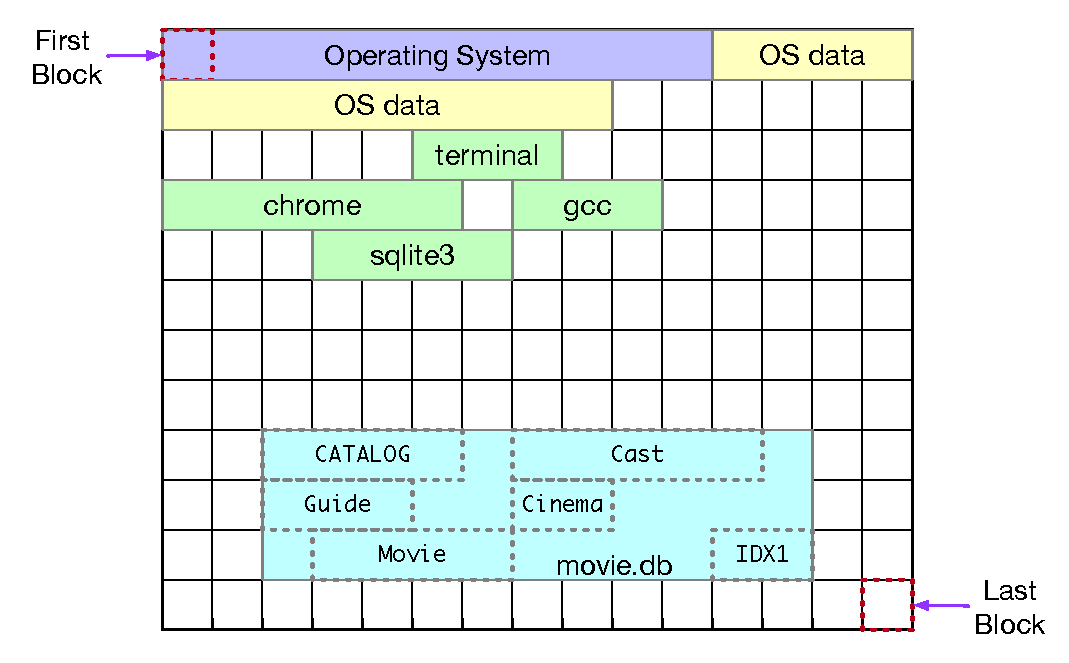
\includegraphics[width=0.9\textwidth]{../lec03_hardware/figures/blocks_on_storage}
\end{center}

These notes are concerned with how the DBMS stores a database on disk and the cost of retrieving data.

\end{frame}


\newsavebox\lecIVsqlExampleONE
\begin{lrbox}{\lecIVsqlExampleONE}
\begin{lstlisting}[style=SQL]
SELECT g.start
FROM Guide g, Cast c
WHERE g.film=c.title AND g.year=c.year
    AND g.theater='Garneau' 
	AND c.actor='Bill Murray'
\end{lstlisting}
\end{lrbox}

\begin{frame}[fragile]

Answering a query requires pulling data from disk to registers (via RAM) so that the CPU can compute the answer.

Some queries require the DBMS to read all tuples from a table:

\begin{center}
\fbox{\lstinline[style=SQL]{SELECT AVG(imdb) FROM Movie}}
\end{center}


\vskip1em
\begin{columns}[onlytextwidth]
\begin{column}{0.5\textwidth}
Most queries, however, require far fewer tuples.\\[0.5em]

For example, only tuples with '\lstinline{Bill Murray}' and '\lstinline{Garneau}' are needed here.
\end{column}
\begin{column}{0.485\textwidth}
\scalebox{0.9}{\fbox{\usebox\lecIVsqlExampleONE}}
\end{column}
\end{columns}

\vskip0.75em

These slides look into methods for storing and/or indexing the data that the database administrator can use to speed up the (queries in the) application.

\end{frame}

\section{Introduction}
%!TEX root = ./lec04_access_methods.tex

\begin{frame}{Database ``files''}

Most DBMSs store an entire database in a single file (as seen by the Operating System)\\
 - recall OS files are collections of blocks of persistent storage

Logically speaking, however, that file is broken down into many components, which in these notes we call ``database files''.

\vskip1em

\begin{center}
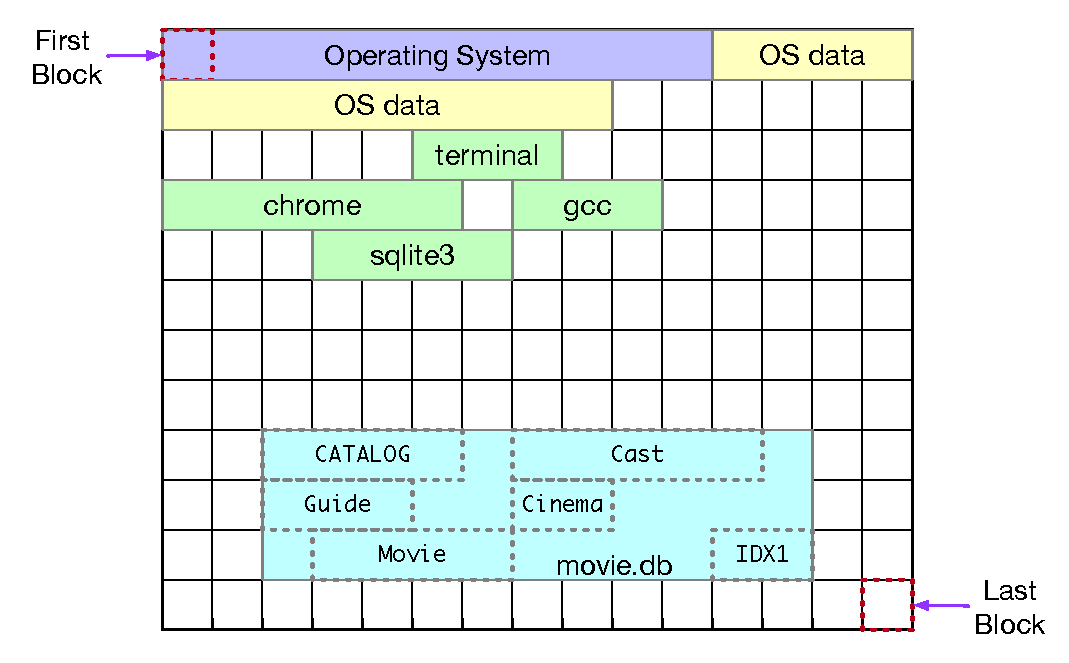
\includegraphics[trim={3.65cm 0.65cm 3.45cm 6.5cm},clip,width=0.6\textwidth]{../lec03_hardware/figures/blocks_on_storage}
\end{center}


Many DBMSs will grab many storage blocks from the Operating System (and leave them empty), to make sure there will be space for growth over time.
\end{frame}


%
% ---------------------------------------------------------------------------
%
\begin{frame}{The database catalog}


The catalog contains the \emph{schemata} of all tables, the description of all indexes and triggers. On multiuser systems, it also contains all users and their privileges.\footnote{Check out the \lstinline[style=cmput391]{-:.schema:-} and \lstinline[style=cmput391]{-:.dump:-} commands in SQLite.}

\vskip1em

The catalog is used all the time: to parse SQL queries, to validate updates, etc. 

Often the DBMS will bring the entire catalog to memory as part of the startup process.

\vskip1em

In most systems, the catalog is actually represented as a collection of tables, which the database administrator can inspect using SQL queries.

\vskip1em

\end{frame}


%
% ---------------------------------------------------------------------------
%
\begin{frame}{Heap files}

The most common kind of DBMS file, called a heap file, is just a \underline{chain of blocks}, with each block containing several \textbf{records}.

Each record represents a database object (e.g., a whole tuple).

\vskip2em

\begin{center}
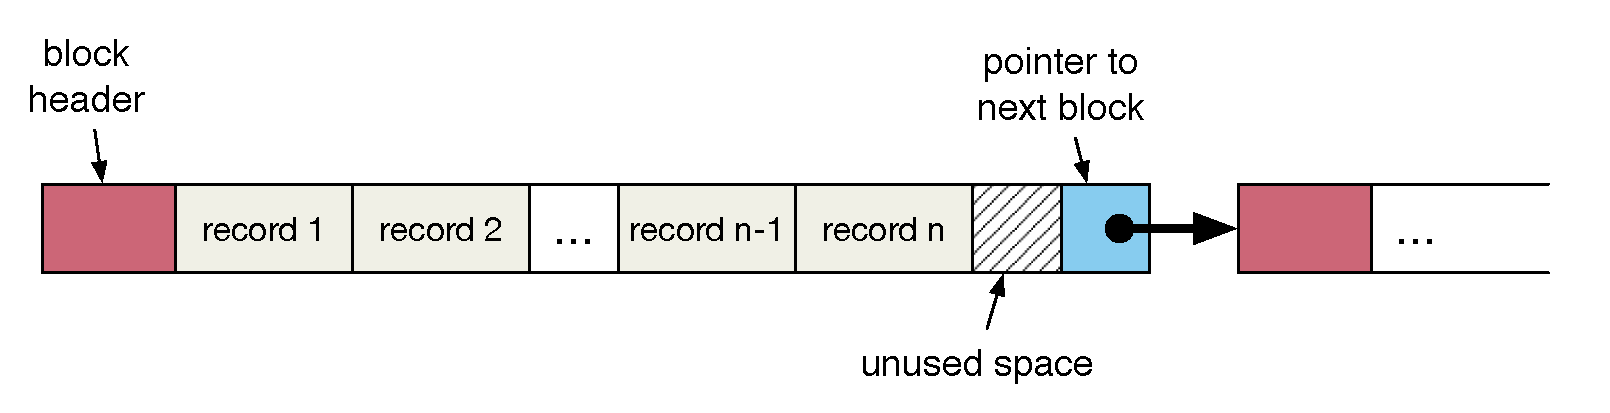
\includegraphics[width=0.9\textwidth]{figures/heap_file}
\end{center}

\end{frame}


%
% ---------------------------------------------------------------------------
%
\begin{frame}

Records have a header (metadata) and a payload (data):

\begin{center}
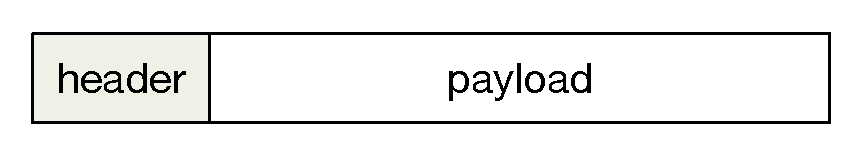
\includegraphics[width=0.5\textwidth]{figures/generic_record}
\end{center}

In a \emph{tuple-oriented store}, each record in a ``table file'' corresponds to a whole tuple\footnote{Except for \lstinline[style=cmput391]{BLOB} (Binary Large OBjects) values like images, sound, etc., in which the record has a pointer to the actual \lstinline[style=cmput391]{BLOB} object.}.

In this case, the header typically contains:
\begin{itemize}[-,noitemsep,topsep=-0.5em]
\item A pointer to the catalog--where the data types of the attributes in the tuple are described.
\item A timestamp of the last update.
\item A flag indicating if the record is valid (or has been deleted).\footnote{It is much cheaper to implement deletions by just marking tuples this way.}
\end{itemize}

\vskip1em
~
\end{frame}


%
% ---------------------------------------------------------------------------
%
\begin{frame}
\label{tuple_oriented_stores}

If the lengths of all attributes in a tuple are defined in the schema, the DBMS can use \textbf{fixed-length records}.

\begin{itemize}[-]
\item In this scheme, every field of the record lies at a constant \emph{offset} from the address where the record is loaded in memory.
\end{itemize}
 

\vskip 0.5em
Example:
\vskip 0.5em

%%% create table stament
\fbox{\usebox{\SimplifiedMovieTableDDL}}

\vskip 0.5em

The record would look like:
\begin{center}
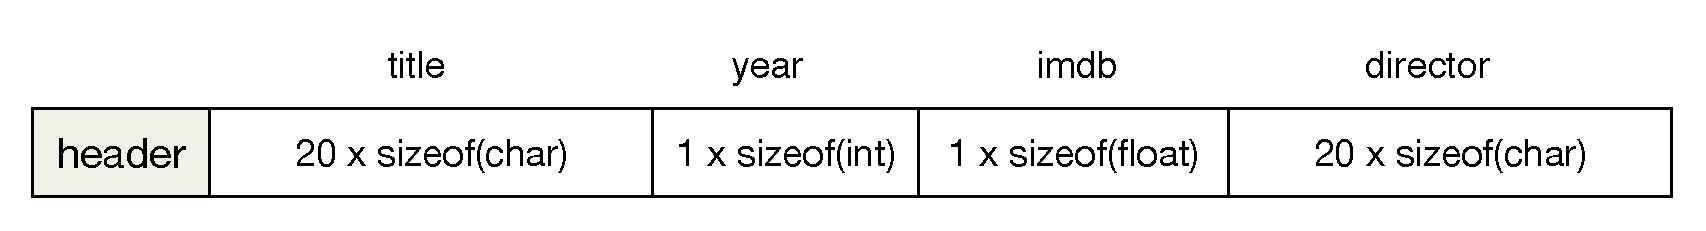
\includegraphics[width=0.95\textwidth]{figures/fixed_record_movie}
\end{center}
\end{frame}


%
% ---------------------------------------------------------------------------
%
\begin{frame}

Fixed-length records can be wasteful for \lstinline[style=SQL]{NULL} values and textual attributes (e.g., names, addresses, etc.) because of variability in the length of actual values.\footnote{SQL has data types for varying-length textual data like \texttt{VARCHAR} and \texttt{TEXT}.}

With \textbf{variable-length} records, instead of ``padding blanks'' special codes as acting as \emph{field delimiters} are used.

\begin{figure}
\begin{subfigure}{0.22\textwidth}
\hfill Fixed
\end{subfigure}
~
\begin{subfigure}{0.74\textwidth}
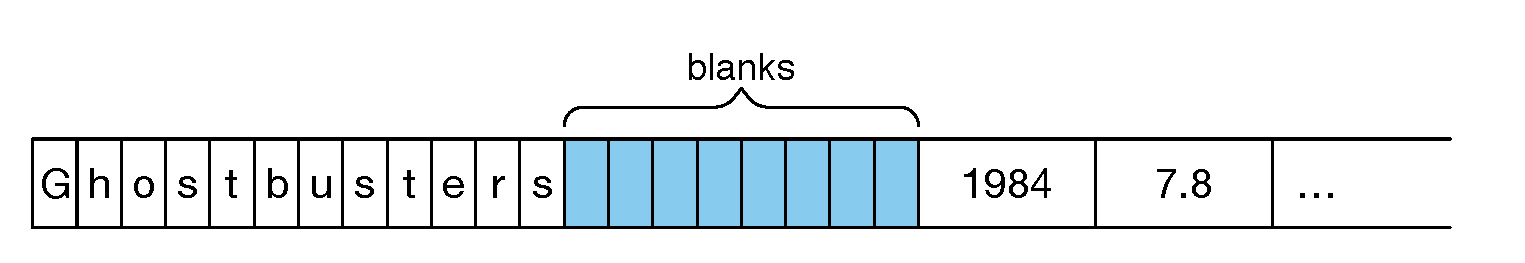
\includegraphics[width=\textwidth]{figures/fixed_length_example}
\end{subfigure}
\end{figure}

\begin{figure}
\begin{subfigure}{0.22\textwidth}
\hfill Variable
\end{subfigure}
~
\begin{subfigure}{0.74\textwidth}
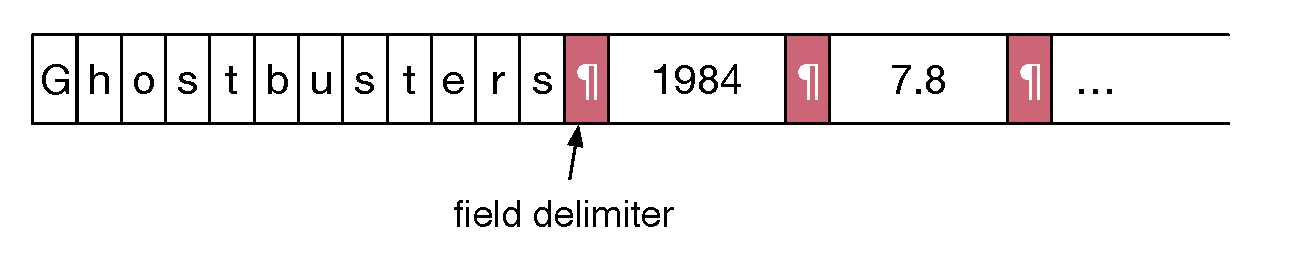
\includegraphics[width=0.85\textwidth]{figures/variable_length_example}
\end{subfigure}
\end{figure}
\end{frame}

%
% ---------------------------------------------------------------------------
%
\begin{frame}

If \lstinline[style=cmput391]{NULL} values are common in the data it is best to use both field delimiters \emph{and} \textbf{field codes}; in this way the record contains only the fields whose values are not missing:

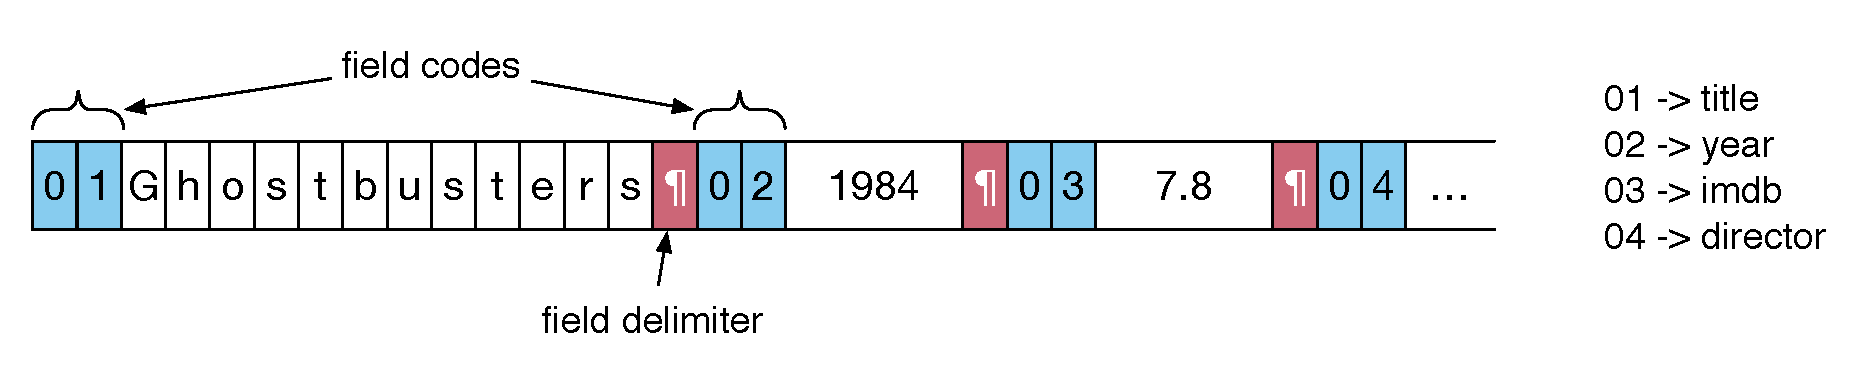
\includegraphics[width=\textwidth]{figures/variable_length_field_codes.eps}

\vskip1em

This kind of record can be used for non-relational data too, like semi-structured or XML.

\end{frame}

%
% ---------------------------------------------------------------------------
%
\begin{frame}{Packing records into buffers/blocks}
\label{heap_file}
Regardless of the kind of record, most stores pack as many whole records into a block as possible. Space that is smaller than a record is \emph{left unused}.

\vskip1em

\begin{center}
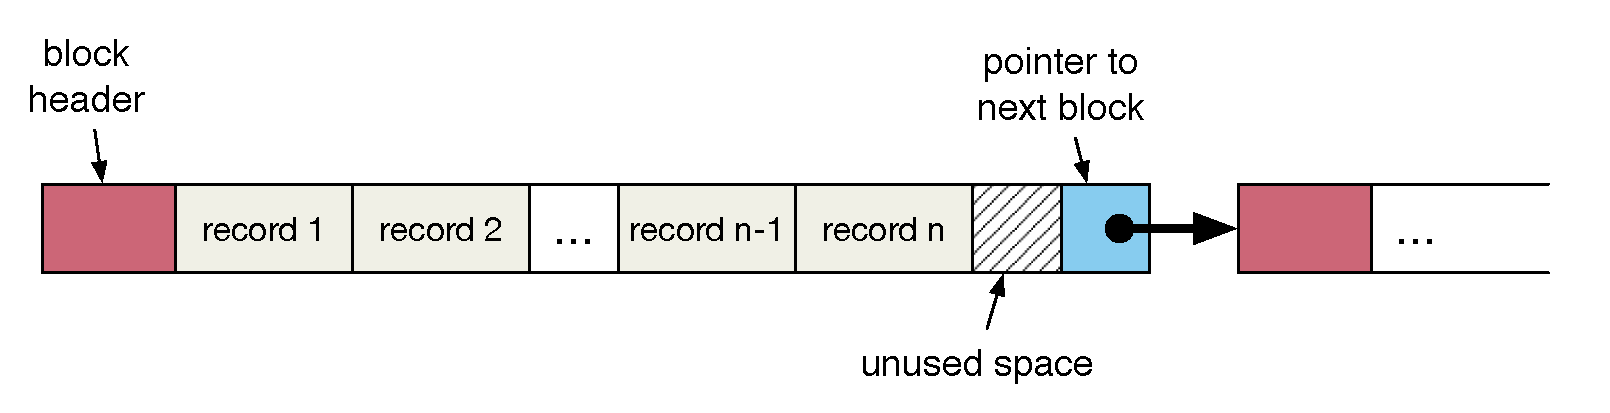
\includegraphics[width=0.9\textwidth]{figures/heap_file}
\end{center}

It is possible to allow a record to \emph{span} consecutive blocks, but the trouble is often not worth it.

\end{frame}


%
% ---------------------------------------------------------------------------
%
\begin{frame}

\textbf{Fixed-length records}:
\begin{itemize}[-,topsep=-0.5em]
\item Fixed number of records per block: \(\floor*{\frac{\text{block size}}{\text{record size}}}\) .

\item Space wasted on ``blanks''.

\item Records and fields start at known \emph{offsets} within the block.
\end{itemize}

\vfill

\textbf{Variable-length records}:

\begin{itemize}[-,topsep=-0.5em]
\item Variable number of records per block.

\item Space ``wasted'' on field separators.

\item Need to scan the whole block to find records and fields.

\item Can be used to store non-relational, semi-structured data.
\end{itemize}

\end{frame}


%
% ---------------------------------------------------------------------------
%
\begin{frame}{ASIDE: word-aligned data structures}
Once a record is loaded in memory, a processor in the CPU can get to a field by manipulating offsets or scanning through the record.

However, some CPUs allow reading/writing entire \textbf{words}\footnote{\url{https://en.wikipedia.org/wiki/Data_structure_alignment}} (4 or 8 bytes, depending on the architecture) only.

When this happens, either the storage stack aligns the fields, which is wasteful,\footnote{Some CPUs, on the other hand, allow access to individual bytes inside each word.} or it contains code to properly ``encode'' and ``decode'' fields into words.
\end{frame}

%
% ---------------------------------------------------------------------------
%
\begin{frame}

Example record:\\
- \texttt{f1}: 5 UTF-16 (2 bytes) characters\\
- \texttt{f2}: 1 Boolean value (1 bit)\\
- \texttt{f3}: 1 \texttt{smallint} (2 bytes)

\begin{figure}
\begin{subfigure}{0.25\textwidth}
\hfill Un-aligned 
\end{subfigure}
~~
\begin{subfigure}{0.7\textwidth}
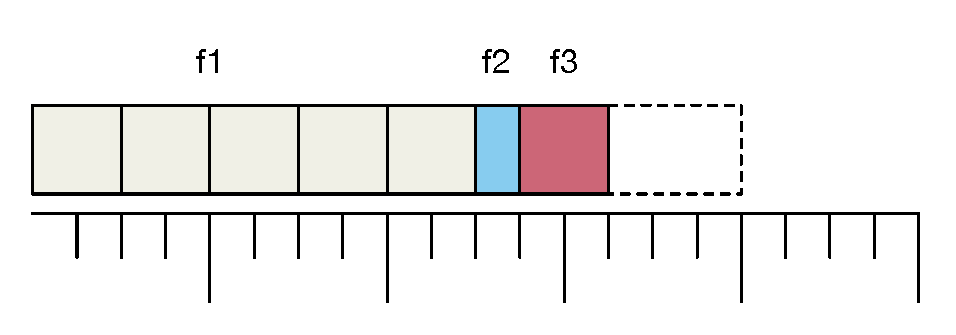
\includegraphics[width=0.8\textwidth]{figures/record_unaligned}
\end{subfigure}
\end{figure}

\begin{figure}
\begin{subfigure}{0.25\textwidth}
\hfill Aligned 
\end{subfigure}
~~
\begin{subfigure}{0.7\textwidth}
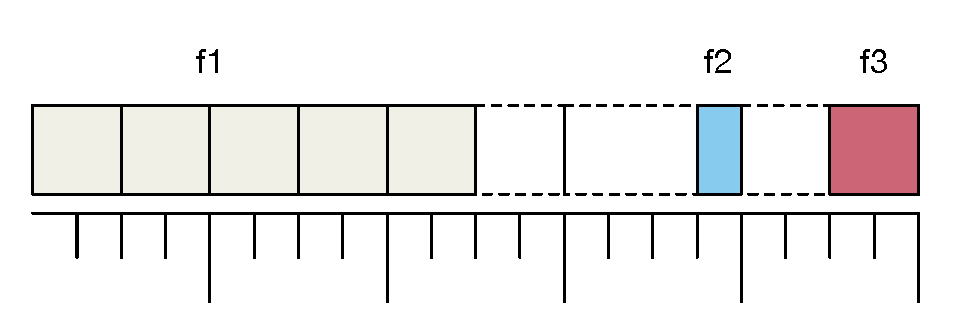
\includegraphics[width=0.8\textwidth]{figures/record_aligned}
\end{subfigure}
\end{figure}

\end{frame}




\section{Heap and Sequential Files}
%!TEX root = ./lec04_access_methods.tex

%
% ---------------------------------------------------------------------------
%
\begin{frame}{Heap Files: Implementation and Access Cost}

Heap files are similar to singly-linked lists, which are easy to maintain. 

\vskip2em 

\begin{center}
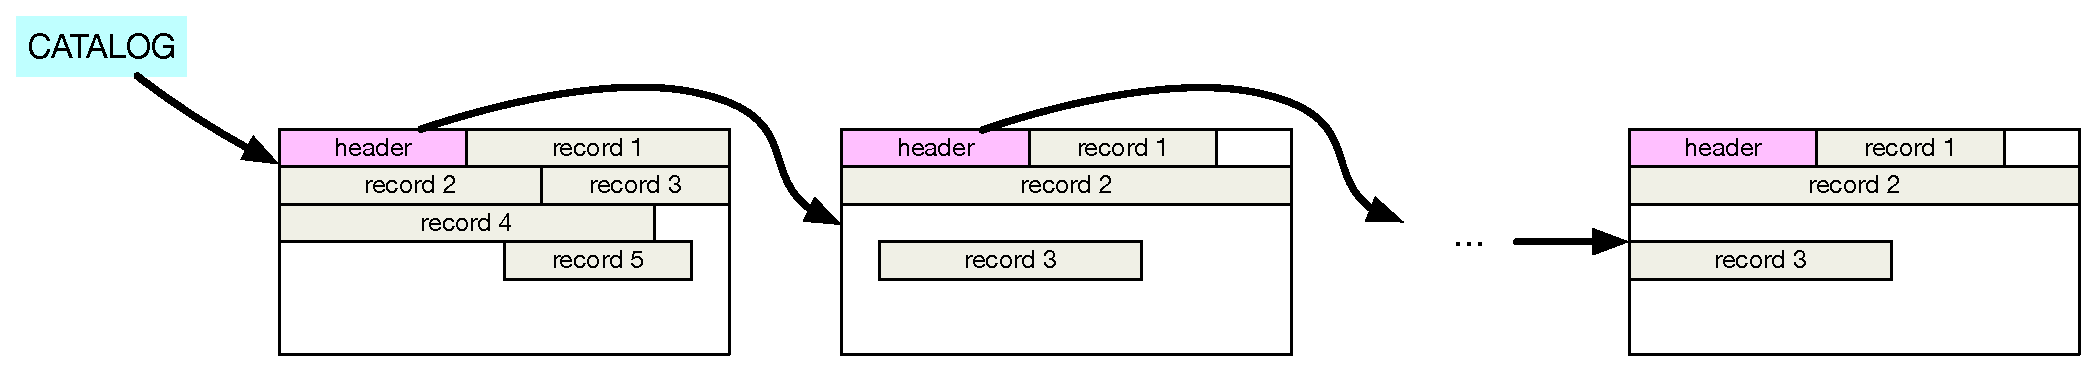
\includegraphics[width=\textwidth]{figures/heap_file_with_catalog.eps}
\end{center}

\vskip1em

All the DBMS needs to record (in the Catalog) is a pointer to the first block in the file.

Each block has its own header for metadata, including, among other things, links to the next block in the chain.

\end{frame}


\begin{frame}{Access costs}

Recall from CMPUT204 that we measure computational costs by in terms of functions that bound \textbf{how many operations} the algorithm requires to complete.

For algorithms dealing with data structures in memory, we typically count accesses to memory.

\vskip1em

\begin{block}{\alert{Computational Cost units}}
Because I/O is so slow, we measure the \textit{cost} as a function of \textbf{how many disk blocks need to be read or written} to perform the operation.
\end{block}
\end{frame}


\begin{frame}

Which kinds of access are supported?

\textbf{Inserting} a new record.

\textbf{Searching} for a record, given a search key.
\begin{itemize}[-,topsep=-0.5em]
\item Example: find movies with \lstinline[style=cmput391]{director='Ivan Reitman'}
\end{itemize}

\textbf{Deleting} or \textbf{updating} a record.

\vskip1em

Note that before we can update or delete a record, we need to first \emph{find} it. The costs for these operations in the following slides will include the search cost. 
\end{frame}


\begin{frame}

\begin{center}
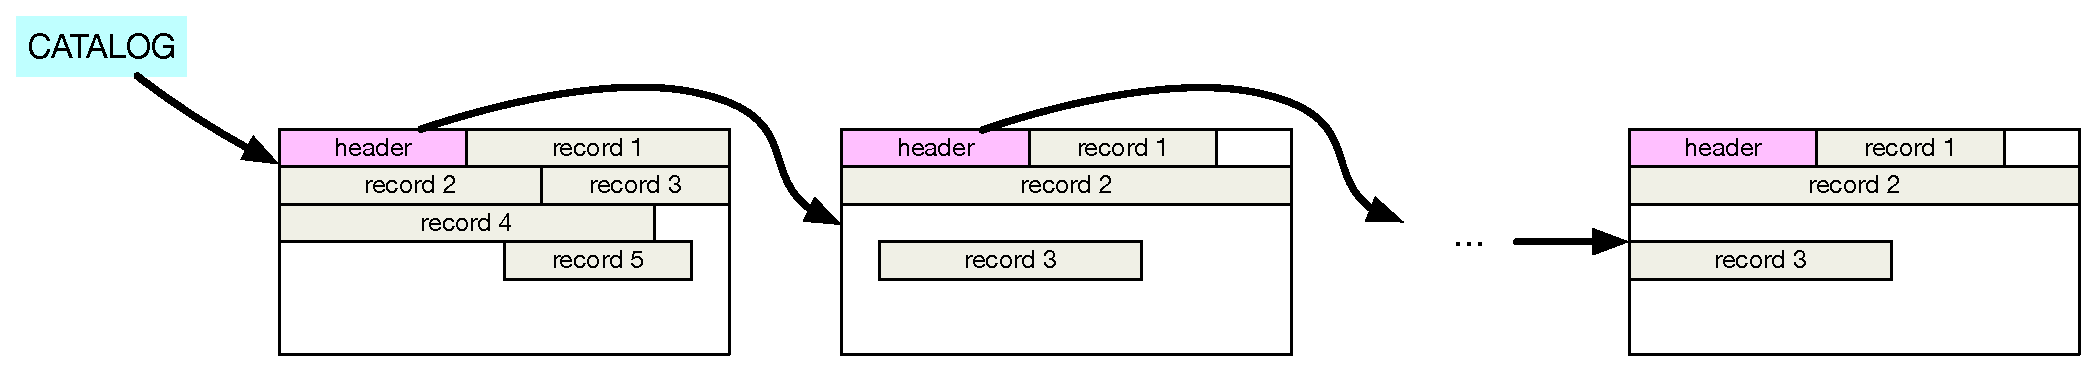
\includegraphics[width=\textwidth]{figures/heap_file_with_catalog.eps}
\end{center}

\textbf{Inserting a new record in a Heap File:}
\begin{itemize}[-,noitemsep,topsep=-0.5em]
\item If there is room in the first block, add the record there.
\item Otherwise, allocate another block to the file, add the record there, and link the new block to the previous first block.
\end{itemize}

\vskip2em

\begin{center}
\fbox{The \textbf{cost} of inserting a new record is $O(1)$}
\end{center}
\end{frame}

%
% ---------------------------------------------------------------------------
%
\begin{frame}

\begin{center}
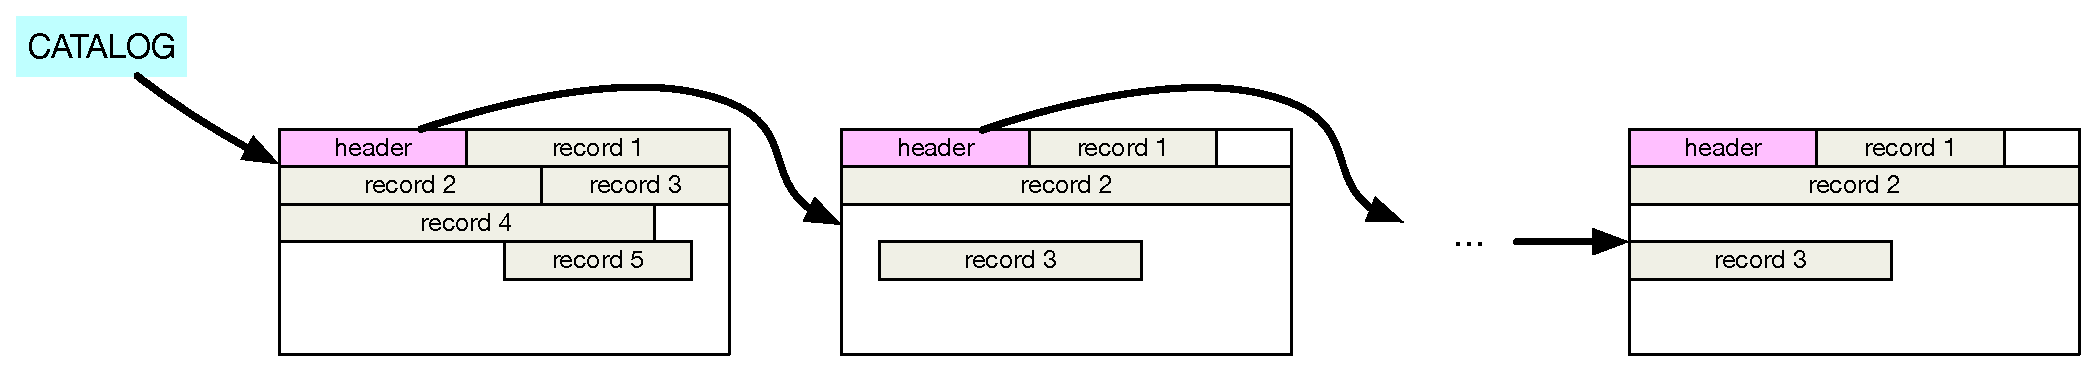
\includegraphics[width=\textwidth]{figures/heap_file_with_catalog.eps}
\end{center}

\vskip1em

\textbf{Searching for a record in a Heap File} with $N$ in blocks.
\begin{itemize}[-,noitemsep,topsep=-0.5em]
\item Traverse all blocks, starting from the first block, following pointers until the record is found (or we exhaust the last block)
\end{itemize}
 
\vskip2em

\begin{center}
\fbox{The \textbf{cost} of finding a record is $O(N)$.}
\end{center}

\end{frame}

\begin{frame}

\begin{center}
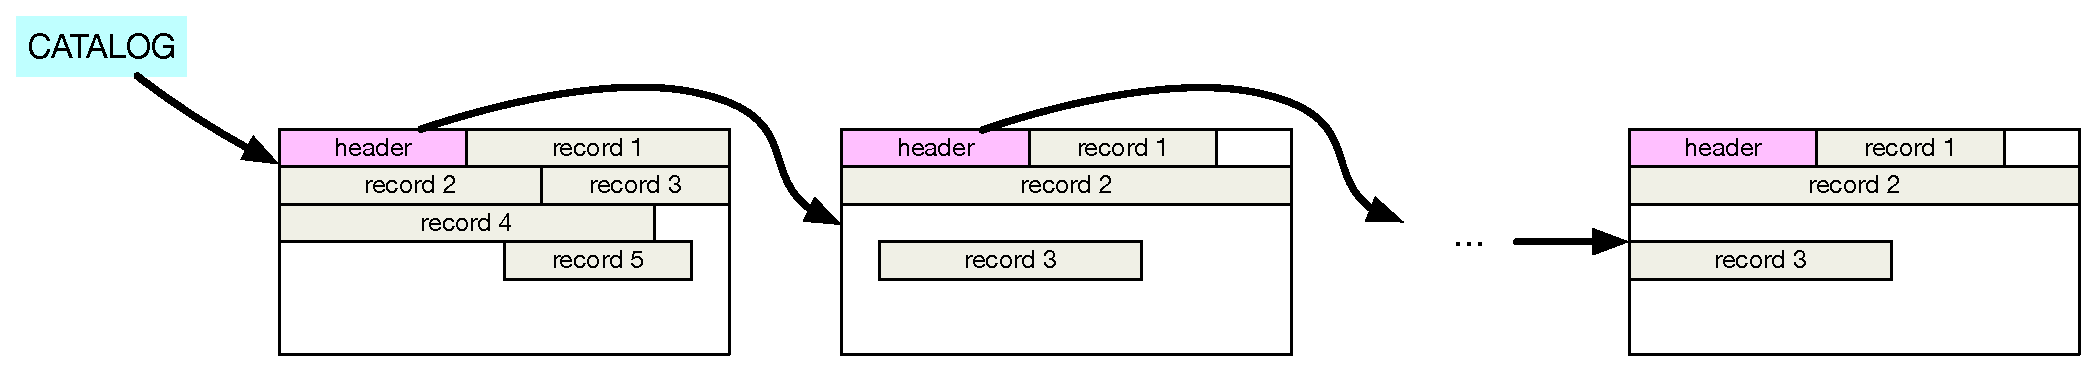
\includegraphics[width=\textwidth]{figures/heap_file_with_catalog.eps}
\end{center}

\vskip1em

\textbf{Deleting or updating a record in a Heap File} with $N$ blocks:
\begin{itemize}[-,noitemsep,topsep=-0.5em]
\item Find the record first (cost $O(N)$), and modify it, or remove it from the block.
\item For deletions: if the block becomes empty, link the previous block to the next in the chain (unless the deletion happens in \emph{last} block).
\end{itemize}

\vskip2em

\begin{center}
\fbox{The \textbf{cost} of deleting a record is $O(N)~$\footnote{Again, because of the search step.}.}
\end{center}
\end{frame}

%
% ------------------------------------------------------------------------------------------------------------------------------
%

\begin{frame}{Sequential Files}


\textbf{Sequential file} are chains of blocks in which the records are \emph{sorted} on a predefined set of attributes, both \emph{within} and \emph{across} blocks.

Tables with primary keys are always stored using sequential files with the primary key as the sorting attributes.

\vskip1em

\begin{columns}[onlytextwidth]
\begin{column}{0.4\textwidth}

Example: sequential file for table \lstinline[style=cmput391]{Movie} sorted by primary key (\lstinline[style=cmput391]{title, year}).

\vskip4em
~

\end{column}
\begin{column}{0.525\textwidth}
\begin{tikzpicture}
\node [anchor=north west] at (0,0) {\scalebox{0.9}{\usebox\SequentialFileMovieTitleYear}};
\end{tikzpicture}
\end{column}
\end{columns}
\end{frame}

%
% ---------------------------------------------------------------------------
%
\begin{frame}{Access cost of Sequential Files}

Searches and deletions are the same as for heap files.

\vskip2em

For \textbf{insertions} on a file with $N$ blocks, we now need to:
\begin{enumerate}[(1),noitemsep,topsep=-0.5em]
\item Find the block where to insert the new record (at cost $O(N)$).
\item Insert the record if there is room, otherwise \alert{rearrange the file}.
\end{enumerate}

\vskip1em

Two ways of rearranging the file:
\begin{itemize}[-,topsep=-0.5em,noitemsep]
\item moving existing records
\item creating a new empty block
\end{itemize}

\end{frame}

%
% ---------------------------------------------------------------------------
%

\begin{frame}{Insertion by rearranging records}

Example: inserting \qquad \raisebox{0.75em}{\scalebox{0.9}{\usebox{\MovieVI}}}

\vskip1em

\begin{columns}[onlytextwidth]
\begin{column}{0.475\textwidth}

\centering \large Before \\[1em]

\begin{tikzpicture}
\node [anchor=south west] at (0,0) {\scalebox{0.8}{\usebox\SequentialFileMovieTitleYear}};
\coordinate (Empty) at (0.2,0.25); 
\coordinate (Wadja) at (0.2,0.5);
\coordinate (LiT) at (0.2,1.25); 
 \path[red, ->,>=stealth'] 
    (Wadja.south) edge[bend right=35] (Empty)
    (LiT) edge[bend right=35] (Wadja.north);
\end{tikzpicture}
\end{column}
\begin{column}{0.475\textwidth}

\centering \large After \\[1em]

\begin{tikzpicture}
\node [anchor=north west] at (0,0) {\scalebox{0.8}{\usebox\SequentialFileMovieTitlYearUpdated}};
\end{tikzpicture}
\end{column}
\end{columns}

\vskip1em

In the worst case scenario, need to keep moving records all the way to the end of the file.

\begin{center}
\fbox{\parbox{0.8\textwidth}{\textbf{cost}: $O(N)$ to rearrange the records in the file; \\~~~~~$O(N)$ to find the block where to make the insertion.}}
\end{center}

\end{frame}


%
% ---------------------------------------------------------------------------
%

\begin{frame}{Insertion by creating a new block}

Example: inserting \qquad \raisebox{0.75em}{\scalebox{0.9}{\usebox{\MovieVI}}}

\vskip2em

\begin{columns}[onlytextwidth]
\begin{column}{0.475\textwidth}

\centering \large Before \\[1em]

\begin{tikzpicture}
\node [anchor=south west] at (0,0) {\scalebox{0.8}{\usebox\SequentialFileMovieTitleYear}};
\end{tikzpicture}
\end{column}
\begin{column}{0.475\textwidth}

\centering \large After \\[1em]

\begin{tikzpicture}
\node [anchor=north west] at (0,0) {\scalebox{0.8}{\usebox\SequentialFileMovieTitlYearUpdatedTWO}};
\end{tikzpicture}
\end{column}
\end{columns}

\vskip1em

\begin{center}
\fbox{\parbox{0.8\textwidth}{\textbf{cost}: $O(1)$ to modify the file; \\~~~~~$O(N)$ to find the block where to make the insertion.}}
\end{center}
\end{frame}

%
% ---------------------------------------------------------------------------
%

\begin{frame}
What about \textbf{updates} to a record in a sequential file?

\vskip1em

\textbf{Case \#1}: The update does not change the sort attributes in the record.
\begin{itemize}[-,topsep=-0.5em]
\item In this case the record remains in the same block as it was\footnote{Unless, of course, the file uses variable length records and the update makes the record too large to fit in the block! In which case a new block must be added to the file.}
\end{itemize} 

\vskip1em

\textbf{Case \#2}: The update does change the sort attributes in the record.
\begin{itemize}[-,topsep=-0.5em]
\item This case is best handled by a deletion of the ``old'' record (before the update) followed by the insertion of the ``new'' record (after the update).
\end{itemize} 

\end{frame}

%
% ---------------------------------------------------------------------------
%

\begin{frame}{Heap vs Sequential Files}
\label{costs_heap_sequential_files}

Both are based on singly-linked lists.

\vskip0.5em

Heap files are better for insertions, but all other operations cost the same in both. If $N$ is the size (in blocks) of the file, then:

\begin{center}
% \large
\begin{tabular}{l | c | c}
& Heap & Sequential\\
\hline\hline
insertion & $O(1)$ & $O(N)$\\
\hline
search & $O(N)$ & $O(N)$\\
\hline
deletion & $O(N)$ & $O(N)$\\
\hline
update & $O(N)$ & $O(N)$
\end{tabular}
\end{center}

\vskip1em

\begin{block}{We need indexes!}
Indexes are needed to cut down the $O(N)$ time to find tuples inside the table file (heap or sequential).
\end{block}

\end{frame}

\begin{frame}

Sequential files can have many quasi-empty blocks after many insertions... which wastes space and (more importantly) I/O operations. 

\vskip1em

\begin{columns}[onlytextwidth]
\begin{column}{0.3\textwidth}
Before:
\end{column}
\begin{column}{0.7\textwidth}
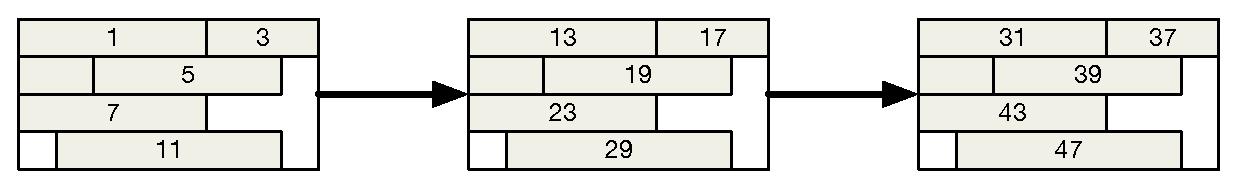
\includegraphics[width=1\textwidth]{figures/seq_file_update_ex1.eps}
\end{column}
\end{columns}

\vskip3em

\pause

\begin{columns}[onlytextwidth]
\begin{column}{0.3\textwidth}
After:
\end{column}
\begin{column}{0.7\textwidth}
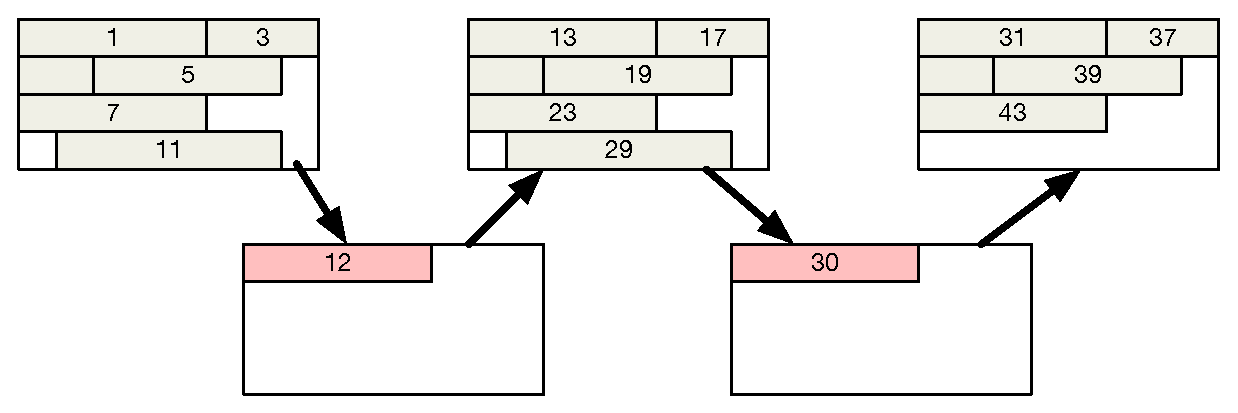
\includegraphics[width=1\textwidth]{figures/seq_file_update_ex2.eps}
\end{column}
\end{columns}

\vskip1em

This can be fixed by \textbf{periodically} taking the database \emph{offline} and re-building the file.

\end{frame}


\section{Indexing Concepts}
%
% Key-pointer measurements
%
\newlength{\indexKeyBoxWidth}
\setlength{\indexKeyBoxWidth}{\dimexpr 2em\relax}

\newlength{\pointerBoxWidth}
\setlength{\pointerBoxWidth}{\dimexpr 2.5em\relax}

%
% Tuple measurements
%
\newlength{\tupleHeight}
\setlength{\tupleHeight}{\dimexpr 1.1em\relax}

\newlength{\dummyTupleGreyBoxWidth}
\setlength{\dummyTupleGreyBoxWidth}{\dimexpr 5em\relax}

%
% Data Block measurements
%

\newlength{\tupleWidth}
\setlength{\tupleWidth}{\dimexpr(\indexKeyBoxWidth+\dummyTupleGreyBoxWidth)\relax}

\newlength{\dataBlockWidth}
\setlength{\dataBlockWidth}{\dimexpr(\tupleWidth+1pt)\relax}

\def\tuplesPerDataBlock{2}

\newlength{\dataBlockHeight}
\setlength{\dataBlockHeight}{\dimexpr1pt+(\tupleHeight+0.5pt)*\the\numexpr\tuplesPerDataBlock\relax}

%
% Index block measurements
%
\newlength{\indexBlockWidth}
\setlength{\indexBlockWidth}{\dimexpr(\indexKeyBoxWidth+\pointerBoxWidth+1pt)\relax}

\def\keyPointerPairsPerIndexBlock{4}

\newlength{\indexBlockHeight}
\setlength{\indexBlockHeight}{\dimexpr1pt+(\tupleHeight+0.5pt)*\the\numexpr\keyPointerPairsPerIndexBlock\relax}

\newlength{\indexBlockPointerOffset}
\setlength{\indexBlockPointerOffset}{\dimexpr(\indexBlockHeight-1em-1pt)\relax}


\tikzset{ % same as tuple, except for the anchor part
	indexKeyBox/.style={
		draw,rectangle,minimum width=\indexKeyBoxWidth,minimum height=\tupleHeight,inner sep=0,outer sep=0,font=\footnotesize
	}
}

\tikzset{
	tupleGrayBox/.style={
		draw, rectangle, minimum width=\dummyTupleGreyBoxWidth,minimum height=\tupleHeight,outer sep=0,fill=tupleBoxColor
	}
}

% #1 --> block id
% #2,#3 --> data block id and order inside block
% #4 --> key
\def\tuple#1#2#3#4{
  \node ({#1}) at ([xshift=1pt,yshift=\dimexpr -1pt-(\tupleHeight+0.5pt)*#3]{#2}.north west) [anchor=north west,indexKeyBox] {{#4}};
  \node [right = -0.5pt of {#1}] [tupleGrayBox] {};
}


% #1 --> block id
% #2,#3 --> data block id and order inside block
% #4 --> key
\def\tupleFromBox#1#2#3#4{
  \node ({#1}) at ([xshift=1pt,yshift=\dimexpr -1pt-(\tupleHeight+0.5pt)*#3]{#2}.north west) [anchor=north west,indexKeyBox] {{#4}};
}


% --------------------------------- index key-pointer tuples

\tikzset{
	keyPointerValue/.style={
		anchor=north west,
		draw,rectangle,minimum width=\indexKeyBoxWidth,minimum height=\tupleHeight,inner sep=0,outer sep=0,font=\footnotesize
	}
}

\tikzset{ 
	keyPointerPointerBox/.style={
		draw, rectangle, minimum width=\pointerBoxWidth,minimum height=\tupleHeight,outer sep=0,fill=snow
	}
}


% #1     --> id of key-pointer (i.e., the node with the value)
% #2, #3 --> id of indexBlock and ordinal within block
% #4     --> value in the attribute of the tuple
\def\keyPointer#1#2#3#4{
  \node ({#1}) at ([xshift=1pt,yshift=\dimexpr -1pt-(\tupleHeight+0.5pt)*#3]{#2}.north west) [anchor=north west,indexKeyBox] {{#4}};
  \node [right = -0.5pt of {#1}] [keyPointerPointerBox] {};
}


% --------------------------------- blocks of the data file

\tikzset{
	dataBlockBox/.style={
		xshift=-0.1em,yshift=0.1em,anchor=north west,draw,rectangle,minimum width=\dataBlockWidth,minimum height=\dataBlockHeight
	}
}

\tikzset{
	dataBlockPointerBox/.style={
		yshift=0.125pt,
		outer sep=0,anchor=south west, draw, rectangle, 
		minimum width=1em, minimum height=1em,fill=snow
	}
}

% #1     --> block id
% #2, #3 --> block top-left coordinates
\def\dataBlock#1#2#3{
	\node ({#1}) at ({#2},{#3}) [dataBlockBox] {};
	\node at ({#1}.south east) [dataBlockPointerBox] {};
}

% #1     --> block id
% #2     --> id of block ``below'' #1
\def\linkDataBlocks#1#2{
	\draw [*->,>=stealth'] ([xshift=5pt,yshift=7pt]{#1}.south east) to[out=270,in=90] ([xshift=-10pt]#2.north east);
}

% --------------------------------- blocks of the index file


\tikzset{
	indexBlockBox/.style={
		xshift=-0.1em,yshift=0.1em,anchor=north west,draw,rectangle,minimum width=\indexBlockWidth,minimum height=\indexBlockHeight
	}
}

\tikzset{
	indexBlockPointerBox/.style={
		xshift=0.375pt,
		anchor=south east, draw, rectangle, minimum width=1em, minimum height=1em,fill=snow
	}
}

% #1     --> block id
% #2, #3 --> block top-left coordinates
% #4     --> id of the first key-pointer inside the block
% #5     --> value of the first key
\def\indexBlock#1#2#3{
	\node ({#1}) at ({#2},{#3}) [indexBlockBox] {};
	\node at ({#1}.south west) [indexBlockPointerBox] {};
}

% #1     --> block id
% #2     --> id of block ``below'' #1
\def\linkIndexBlocks#1#2{
	\draw [*->,>=stealth'] ([xshift=-5pt,yshift=7pt]{#1}.south west) to[out=270,in=90] ([xshift=10pt]#2.north west);
}

% #1 --> key-pointer id
% #2 --> tuple id
\def\KPtoTuple#1#2{
	\draw [*->,>=stealth'] ([xshift=30pt,yshift=0em]{#1}.west) to[out=0,in=180] (#2.west);
}




%%%%% MACROS FOR SPARSE INDEX WITH POINTERS TO BLOCKS

\tikzset{ 
	sparseKeyPointerPointerBox/.style={
		draw, rectangle, minimum width=1.1em,minimum height=\tupleHeight, fill=snow
	}
}

% draws two rectangles, one with an attribute value, the other with the pointer
%
% #1     --> id of key-pointer (i.e., the node with the value)
% #2, #3 --> coordinages of top-left corner of node with tuple value
% #4     --> value in the attribute of the tuple
\def\sparseKeyPointer#1#2#3#4{
  \node ({#1}) at ({#2},{#3}) [keyPointerValue] {\tiny{#4}} ;
  \node [right = -0.5pt of {#1}] [sparseKeyPointerPointerBox] {};
}

\tikzset{
	sparseIndexBlockBox/.style={
		xshift=-0.1em,yshift=0.1em,anchor=north west,draw,rectangle,minimum width=3.3em,minimum height=4.6em
	}
}

% #1     --> block id
% #2, #3 --> block top-left coordinates
% #4     --> id of the first key-pointer inside the block
% #5     --> value of the first key
\def\sparseIndexBlock#1#2#3#4#5{
	\node ({#1}) at ({#2},{#3}) [sparseIndexBlockBox] {};
	\node at ({#2},{#3}) [indexBlockPointerBox] {};
	\sparseKeyPointer{{#4}}{{#2}}{{#3}}{{#5}};
}

% #1     --> block id
% #2     --> id of block ``above'' this one
% #3, #4 --> coordinates of this block
% #5     --> id of the first tuple inside the block
% #6     --> value of the first tuple
\def\sparseIndexBlockBelow#1#2#3#4#5#6{
	\node ({#1}) at ({#3},{#4}) [sparseIndexBlockBox] {};
	\node at ({#3},{#4}) [indexBlockPointerBox] {};
	\sparseKeyPointer{{#5}}{{#3}}{{#4}}{{#6}};
	\draw [*->,>=stealth'] ([xshift=-5pt,yshift=7pt]{#2}.south west) to[out=270,in=90] ([xshift=10pt]#1.north west);
}

% #1 --> key-pointer id
% #2 --> tuple id
\def\sparseKPtoTuple#1#2{
	\draw [*->,>=stealth'] ([xshift=22.5pt,yshift=0em]{#1}.west) to[out=0,in=180] (#2.west);
}



%================================ illustration of multilevel indexes

\def\denseIndexMultilevel#1#2#3#4{
    \node ({#1}) at ({#2},{#3}) [font=\footnotesize,draw,fill=accent!25,rectangle,minimum width=2.5em,minimum height=1em] {{#4}};
    \node (t) [below = 1em of {#1}] [rectangle,minimum width=2.5em] {};
    \draw [->,>=stealth'] ({#1}) -- (t);
    \draw [->,>=stealth'] ([xshift=-2pt]{#1}.south) -- ([xshift=-6pt]t.north);
    \draw [->,>=stealth'] ([xshift=2pt]{#1}.south) -- ([xshift=6pt]t.north);
    \draw [->,>=stealth'] ([xshift=-6pt]{#1}.south) -- (t.north west);
    \draw [->,>=stealth'] ([xshift=6pt]{#1}.south) -- (t.north east);
}

\def\denseIndexMultilevelAfter#1#2#3{
    \node ({#1}) [right of= {#2}] [font=\footnotesize,draw,fill=accent!25,rectangle,minimum width=2.5em,minimum height=1em] {{#3}};
        \node (t) [below = 1em of {#1}] [rectangle,minimum width=2.5em] {};
    \draw [->,>=stealth'] ({#1}) -- (t);
    \draw [->,>=stealth'] ([xshift=-2pt]{#1}.south) -- ([xshift=-6pt]t.north);
    \draw [->,>=stealth'] ([xshift=2pt]{#1}.south) -- ([xshift=6pt]t.north);
    \draw [->,>=stealth'] ([xshift=-6pt]{#1}.south) -- (t.north west);
    \draw [->,>=stealth'] ([xshift=6pt]{#1}.south) -- (t.north east);
}


\newsavebox\genericDenseIndexWithNblocks
\savebox{\genericDenseIndexWithNblocks}{
\begin{tikzpicture}[
	every node/.append style={node distance=4em},
	every edge/.append style={>=stealth'}]
\node at (-1.5,0) [color=accent,font=\footnotesize] {Index:};

\denseIndexMultilevel{0}{0}{0}{$b_0$};
\denseIndexMultilevelAfter{1}{0}{$b_1$};
\denseIndexMultilevelAfter{2}{1}{$b_2$};
\node (3) [right of=2] {...};
\denseIndexMultilevelAfter{4}{3}{$b_{N-1}$};
\denseIndexMultilevelAfter{5}{4}{$b_{N}$};

\path [->] (0) edge (1) 
   (1) edge (2)
   (2) edge (3)
   (3) edge (4)
   (4) edge (5);
\end{tikzpicture}
}

\newsavebox\genericMultilevelIndexSparseOnDense
\savebox{\genericMultilevelIndexSparseOnDense}{
\begin{tikzpicture}[
	every node/.append style={node distance=4em},
	every edge/.append style={>=stealth'}]
\tikzset{
    block/.style={font=\footnotesize,draw,fill=snow,rectangle,minimum width=2.5em,minimum height=1em}
    }
\tikzset{
    sparseBlock/.style={font=\footnotesize,draw,fill=snow,rectangle,minimum width=2.5em,minimum height=1em}
    }

\node at (-1.5,0) [color=accent,font=\footnotesize] {\begin{minipage}{1cm}\baselineskip=0.75\baselineskip \centering
Dense Index: \end{minipage}};

\denseIndexMultilevel{0}{0}{0}{$b_0$};
\denseIndexMultilevelAfter{1}{0}{$b_1$};
\denseIndexMultilevelAfter{2}{1}{$b_2$};
\node (3) [right of=2] {...};
\denseIndexMultilevelAfter{4}{3}{$b_{N-1}$};
\denseIndexMultilevelAfter{5}{4}{$b_{N}$};

\path [->] (0) edge (1) 
   (1) edge (2)
   (2) edge (3)
   (3) edge (4)
   (4) edge (5);

\node at (-1.5,1.5) [color=accent,font=\footnotesize] {\begin{minipage}{1cm}\baselineskip=0.75\baselineskip \centering
Sparse Index: \end{minipage}};

\node [sparseBlock] (6) [xshift=1em,above of=1] {$\mathit{b}_0$};
\node (7) [xshift=1em,right of=6] {...};
\node [sparseBlock] (8) [xshift=1em,right of=7] {$\mathit{b}_M$};

\path [->] (6) edge (7)
    (7) edge (8);

\draw [->,>=stealth'] ([xshift=-9pt]6.south) to[out=270,in=90] ([xshift=2pt]0.north west);
\draw [->,>=stealth'] ([xshift=-5pt]6.south) to[out=270,in=90] ([xshift=2pt]1.north west);
\draw [->,>=stealth'] ([xshift=-1pt]6.south) to[out=270,in=90] ([xshift=2pt]2.north west);
\draw [->,>=stealth'] ([xshift=5pt]8.south) to[out=270,in=90] ([xshift=2pt]4.north west);
\draw [->,>=stealth'] ([xshift=9pt]8.south) to[out=270,in=90] ([xshift=2pt]5.north west);

\node (inv1) [xshift=2em,yshift=-1em,above right of=1,rectangle]  {...};
\draw [->,>=stealth'] ([xshift=2pt]6.south) -- (inv1.north west);
\draw [->,>=stealth'] ([xshift=9pt]6.south) -- (inv1.north east);

\node (inv2) [xshift=-2em,yshift=-1em,above right of=3,rectangle]  {...};
\draw [->,>=stealth'] ([xshift=-4pt]8.south) -- (inv2.north east);
\draw [->,>=stealth'] ([xshift=-8pt]8.south) -- (inv2.north west);
\end{tikzpicture}
}


%
% illustration scanning cost of range selection on dense primary index
%

\newsavebox{\rangeSelectionQueryPrimaryIndex}
\savebox{\rangeSelectionQueryPrimaryIndex}{
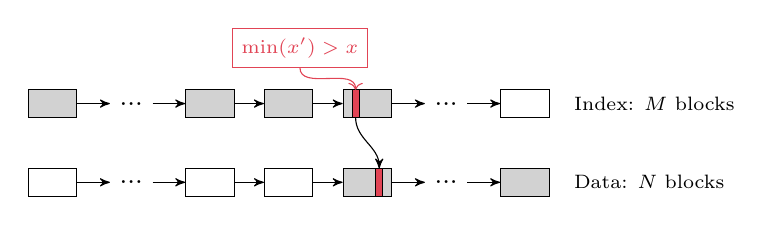
\begin{tikzpicture}
%index blocks
\node (0) at (0,0) [draw,rectangle,fill=gray!35,minimum width=1.75em,minimum height=1em] {};
\node (1) at (1,0) [rectangle,minimum width=1em,minimum height=1em] {...};
\foreach \i in {2,...,4}{
  \node (\i) at (\i,0) [draw,rectangle,fill=gray!35,minimum width=1.75em,minimum height=1em] {};  
}
\node (5) at (5,0) [rectangle,minimum width=1em,minimum height=1em] {...};    
\node (6) at (6,0) [draw,rectangle,minimum width=1.75em,minimum height=1em] {};
%chain of index blocks
\foreach \i in {1,...,6}{
    {\pgfmathsetmacro{\j}{\i - 1}
    \draw [->,>=stealth'] ({\j}) -- (\i);}
}

%data blocks
\node (7) at (0,-1) [draw,rectangle,minimum width=1.75em,minimum height=1em] {};
\node (8) at (1,-1) [rectangle,minimum width=1em,minimum height=1em] {...};
\foreach \i in {9,...,10}{
  \pgfmathsetmacro{\j}{\i - 7}
  \node (\i) at (\j,-1) [draw,rectangle,minimum width=1.75em,minimum height=1em] {};  
}
\node (11) at (4,-1) [draw,rectangle,fill=gray!35,minimum width=1.75em,minimum height=1em] {};
\node (12) at (5,-1) [rectangle,minimum width=1em,minimum height=1em] {...};    
\node (13) at (6,-1) [draw,rectangle,fill=gray!35,minimum width=1.75em,minimum height=1em] {};
%chain of data blocks
\foreach \i in {8,...,13}{
    {\pgfmathsetmacro{\j}{\i - 1}
    \draw [->,>=stealth'] ({\j}) -- (\i);}
}

%index and tuple keys
\node (k) at (3.85,0) [inner sep=0,outer sep=0,draw,fill=accent,rectangle,minimum width=0.25em,minimum height=1em] {};
\node (t) at (4.15,-1) [inner sep=0,outer sep=0,draw,fill=accent,rectangle,minimum width=0.25em,minimum height=1em] {};

%labels
\node (i) [outer sep=0pt,above left of=k,draw,color=accent] {\scriptsize $\min (x') > x$};
\node at (6.5,-1) [anchor= west]{\scriptsize Data: $N$ blocks}; 
\node at (6.5,0) [anchor= west]{\scriptsize Index: $M$ blocks}; 

\draw [color=accent,->] (i.south) to[out=270,in=90] (k.north);
\draw [->,>=stealth'] (k.south) to[out=270,in=90] (t.north);
\end{tikzpicture}
}


%
%
% --------------------------------------------------------------
%
%


\newsavebox{\rangeSelectionQueryStackedIndex}
\savebox{\rangeSelectionQueryStackedIndex}{
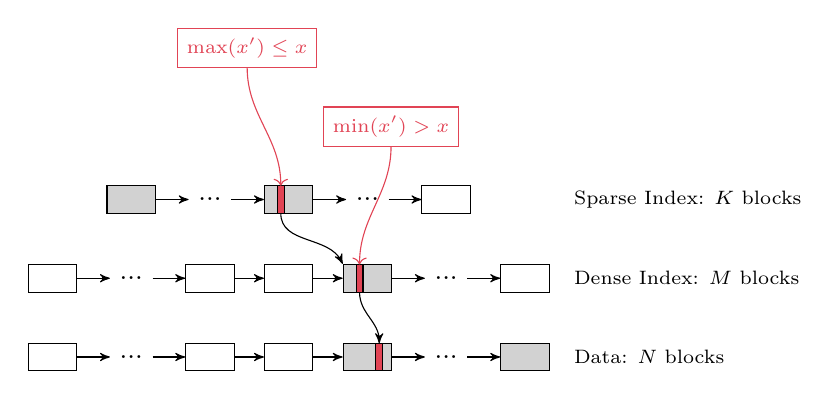
\begin{tikzpicture}
%index blocks
\node (0) at (0,0) [draw,rectangle,,minimum width=1.75em,minimum height=1em] {};
\node (1) at (1,0) [rectangle,minimum width=1em,minimum height=1em] {...};
\foreach \i in {2,...,3}{
  \node (\i) at (\i,0) [draw,rectangle,minimum width=1.75em,minimum height=1em] {};  
}
\node (4) at (4,0) [draw,rectangle,fill=gray!35,minimum width=1.75em,minimum height=1em] {};
\node (5) at (5,0) [rectangle,minimum width=1em,minimum height=1em] {...};    
\node (6) at (6,0) [draw,rectangle,minimum width=1.75em,minimum height=1em] {};
%chain of index blocks
\foreach \i in {1,...,6}{
    {\pgfmathsetmacro{\j}{\i - 1}
    \draw [->,>=stealth'] ({\j}) -- (\i);}
}

%sparse index on top of dense index
\node (14) at (1,1) [draw,rectangle,fill=gray!35,minimum width=1.75em,minimum height=1em] {};
\node (15) at (2,1)  {...};
\node (16) at (3,1) [draw,rectangle,fill=gray!35,minimum width=1.75em,minimum height=1em] {};
\node (17) at (4,1)  {...};
\node (18) at (5,1) [draw,rectangle,minimum width=1.75em,minimum height=1em] {};
\foreach \i in {15,...,18}{
    {\pgfmathsetmacro{\j}{\i - 1}
    \draw [->,>=stealth'] ({\j}) -- (\i);}
}

%data blocks
\node (7) at (0,-1) [draw,rectangle,minimum width=1.75em,minimum height=1em] {};
\node (8) at (1,-1) [rectangle,minimum width=1em,minimum height=1em] {...};
\foreach \i in {9,...,10}{
  \pgfmathsetmacro{\j}{\i - 7}
  \node (\i) at (\j,-1) [draw,rectangle,minimum width=1.75em,minimum height=1em] {};  
}
\node (11) at (4,-1) [draw,rectangle,fill=gray!35,minimum width=1.75em,minimum height=1em] {};
\node (12) at (5,-1) [rectangle,minimum width=1em,minimum height=1em] {...};    
\node (13) at (6,-1) [draw,rectangle,fill=gray!35,minimum width=1.75em,minimum height=1em] {};
%chain of data blocks
\foreach \i in {8,...,13}{
    {\pgfmathsetmacro{\j}{\i - 1}
    \draw [->,>=stealth'] ({\j}) -- (\i);}
}

%index and tuple keys
\node (k) at (3.9,0) [inner sep=0,outer sep=0,draw,fill=accent,rectangle,minimum width=0.25em,minimum height=1em] {};
\node (s) at (2.9,1) [inner sep=0,outer sep=0,draw,fill=accent,rectangle,minimum width=0.25em,minimum height=1em] {};
\node (t) at (4.15,-1) [inner sep=0,outer sep=0,draw,fill=accent,rectangle,minimum width=0.25em,minimum height=1em] {};

%labels
\node (i) [outer sep=0pt,above left=1.5cm and -0.5cm of s,draw,color=accent] {\scriptsize $\max (x') \leq x$};
\node (j) [outer sep=0pt,above right=1.5cm and -0.5cm of k,draw,color=accent] {\scriptsize $\min (x') > x$};
\node at (6.5,-1) [anchor= west]{\scriptsize Data: $N$ blocks}; 
\node at (6.5,0) [anchor= west]{\scriptsize Dense Index: $M$ blocks}; 
\node at (6.5,1) [anchor= west]{\scriptsize Sparse Index: $K$ blocks}; 

\draw [color=accent,->] (j.south) to[out=270,in=90] (k.north);
\draw [color=accent,->] (i.south) to[out=270,in=90] (s.north);

\draw [->,>=stealth'] (s.south) to[out=270,in=115] (4.north west);
\draw [->,>=stealth'] (k.south) to[out=270,in=90] (t.north);
\end{tikzpicture}
}


%
%
% --------------------------------------------------------------
%
%

\newsavebox{\rangeSelectionQuerySecondaryIndex}
\savebox{\rangeSelectionQuerySecondaryIndex}{
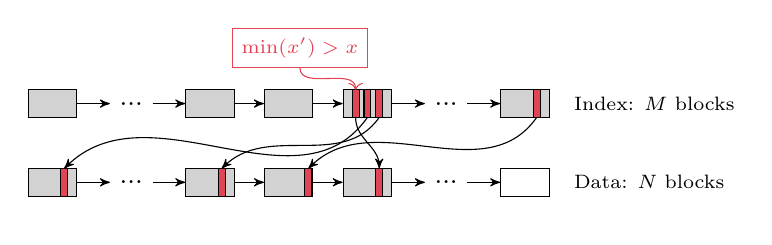
\begin{tikzpicture}
%index blocks
\node (0) at (0,0) [draw,rectangle,fill=gray!35,minimum width=1.75em,minimum height=1em] {};
\node (1) at (1,0) [rectangle,minimum width=1em,minimum height=1em] {...};
\foreach \i in {2,...,4}{
  \node (\i) at (\i,0) [draw,rectangle,fill=gray!35,minimum width=1.75em,minimum height=1em] {};  
}
\node (5) at (5,0) [rectangle,minimum width=1em,minimum height=1em] {...};    
\node (6) at (6,0) [draw,rectangle,fill=gray!35,minimum width=1.75em,minimum height=1em] {};
%chain of index blocks
\foreach \i in {1,...,6}{
    {\pgfmathsetmacro{\j}{\i - 1}
    \draw [->,>=stealth'] ({\j}) -- (\i);}
}

%data blocks
\node (7) at (0,-1) [draw,rectangle,fill=gray!35,minimum width=1.75em,minimum height=1em] {};
\node (8) at (1,-1) [rectangle,minimum width=1em,minimum height=1em] {...};
\foreach \i in {9,...,10}{
  \pgfmathsetmacro{\j}{\i - 7}
  \node (\i) at (\j,-1) [draw,rectangle,fill=gray!35,minimum width=1.75em,minimum height=1em] {};  
}
\node (11) at (4,-1) [draw,rectangle,fill=gray!35,minimum width=1.75em,minimum height=1em] {};
\node (12) at (5,-1) [rectangle,minimum width=1em,minimum height=1em] {...};    
\node (13) at (6,-1) [draw,rectangle,minimum width=1.75em,minimum height=1em] {};
%chain of data blocks
\foreach \i in {8,...,13}{
    {\pgfmathsetmacro{\j}{\i - 1}
    \draw [->,>=stealth'] ({\j}) -- (\i);}
}

%index and tuple keys
\node (k) at (3.85,0) [inner sep=0,outer sep=0,draw,fill=accent,rectangle,minimum width=0.25em,minimum height=1em] {};
\node (t) at (4.15,-1) [inner sep=0,outer sep=0,draw,fill=accent,rectangle,minimum width=0.25em,minimum height=1em] {};

%labels
\node (i) [outer sep=0pt,above left of=k,draw,color=accent] {\scriptsize $\min (x') > x$};
\node at (6.5,-1) [anchor= west]{\scriptsize Data: $N$ blocks}; 
\node at (6.5,0) [anchor= west]{\scriptsize Index: $M$ blocks}; 

\draw [color=accent,->] (i.south) to[out=270,in=90] (k.north);
\draw [->,>=stealth'] (k.south) to[out=270,in=90] (t.north);

% out of order keys/tuples
\node (k2) at (4,0) [inner sep=0,outer sep=0,draw,fill=accent,rectangle,minimum width=0.25em,minimum height=1em] {};
\node (t2) at (0.15,-1) [inner sep=0,outer sep=0,draw,fill=accent,rectangle,minimum width=0.25em,minimum height=1em] {};
\draw [->,>=stealth'] (k2.south) to[out=235,in=45] (t2.north);

\node (k3) at (4.15,0) [inner sep=0,outer sep=0,draw,fill=accent,rectangle,minimum width=0.25em,minimum height=1em] {};
\node (t3) at (2.15,-1) [inner sep=0,outer sep=0,draw,fill=accent,rectangle,minimum width=0.25em,minimum height=1em] {};
\draw [->,>=stealth'] (k3.south) to[out=235,in=45] (t3.north);

\node (k4) at (6.15,0) [inner sep=0,outer sep=0,draw,fill=accent,rectangle,minimum width=0.25em,minimum height=1em] {};
\node (t4) at (3.25,-1) [inner sep=0,outer sep=0,draw,fill=accent,rectangle,minimum width=0.25em,minimum height=1em] {};
\draw [->,>=stealth'] (k4.south) to[out=235,in=45] (t4.north);

\end{tikzpicture}
}



%
%
% --------------------------------------------------------------
%
%

\newsavebox{\motivatingBucketFiles}
\savebox{\motivatingBucketFiles}{
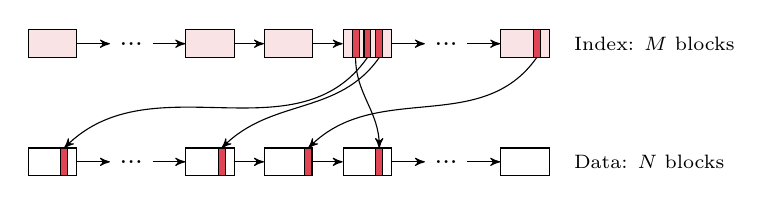
\begin{tikzpicture}
%index blocks
\node (0) at (0,0) [draw,rectangle,fill=accent!15,minimum width=1.75em,minimum height=1em] {};
\node (1) at (1,0) [rectangle,minimum width=1em,minimum height=1em] {...};
\foreach \i in {2,...,4}{
  \node (\i) at (\i,0) [draw,rectangle,fill=accent!15,minimum width=1.75em,minimum height=1em] {};  
}
\node (5) at (5,0) [rectangle,minimum width=1em,minimum height=1em] {...};    
\node (6) at (6,0) [draw,rectangle,fill=accent!15,minimum width=1.75em,minimum height=1em] {};
%chain of index blocks
\foreach \i in {1,...,6}{
    {\pgfmathsetmacro{\j}{\i - 1}
    \draw [->,>=stealth'] ({\j}) -- (\i);}
}

%data blocks
\node (7) at (0,-1.5) [draw,rectangle,minimum width=1.75em,minimum height=1em] {};
\node (8) at (1,-1.5) [rectangle,minimum width=1em,minimum height=1em] {...};
\foreach \i in {9,...,10}{
  \pgfmathsetmacro{\j}{\i - 7}
  \node (\i) at (\j,-1.5) [draw,rectangle,minimum width=1.75em,minimum height=1em] {};  
}
\node (11) at (4,-1.5) [draw,rectangle,minimum width=1.75em,minimum height=1em] {};
\node (12) at (5,-1.5) [rectangle,minimum width=1em,minimum height=1em] {...};    
\node (13) at (6,-1.5) [draw,rectangle,minimum width=1.75em,minimum height=1em] {};
%chain of data blocks
\foreach \i in {8,...,13}{
    {\pgfmathsetmacro{\j}{\i - 1}
    \draw [->,>=stealth'] ({\j}) -- (\i);}
}

%index and tuple keys
\node (k) at (3.85,0) [inner sep=0,outer sep=0,draw,fill=accent,rectangle,minimum width=0.25em,minimum height=1em] {};
\node (t) at (4.15,-1.5) [inner sep=0,outer sep=0,draw,fill=accent,rectangle,minimum width=0.25em,minimum height=1em] {};

%labels
\node at (6.5,-1.5) [anchor= west]{\scriptsize Data: $N$ blocks}; 
\node at (6.5,0) [anchor= west]{\scriptsize Index: $M$ blocks}; 

\draw [->,>=stealth'] (k.south) to[out=270,in=90] (t.north);

% out of order keys/tuples
\node (k2) at (4,0) [inner sep=0,outer sep=0,draw,fill=accent,rectangle,minimum width=0.25em,minimum height=1em] {};
\node (t2) at (0.15,-1.5) [inner sep=0,outer sep=0,draw,fill=accent,rectangle,minimum width=0.25em,minimum height=1em] {};
\draw [->,>=stealth'] (k2.south) to[out=235,in=45] (t2.north);

\node (k3) at (4.15,0) [inner sep=0,outer sep=0,draw,fill=accent,rectangle,minimum width=0.25em,minimum height=1em] {};
\node (t3) at (2.15,-1.5) [inner sep=0,outer sep=0,draw,fill=accent,rectangle,minimum width=0.25em,minimum height=1em] {};
\draw [->,>=stealth'] (k3.south) to[out=235,in=45] (t3.north);

\node (k4) at (6.15,0) [inner sep=0,outer sep=0,draw,fill=accent,rectangle,minimum width=0.25em,minimum height=1em] {};
\node (t4) at (3.25,-1.5) [inner sep=0,outer sep=0,draw,fill=accent,rectangle,minimum width=0.25em,minimum height=1em] {};
\draw [->,>=stealth'] (k4.south) to[out=235,in=45] (t4.north);

\end{tikzpicture}
}

%!TEX root = ./lec04_access_methods.tex

%
% -----------------------------------------------------------------------
%
\begin{frame}[fragile]{Indexes Are Associative Data Structures}

An index is an \alert{\textbf{associative data structure}} (stored on disk) that allows the DBMS to find tuples that satisfy a predicate defined over a subset of the attributes in the tuple.

Index declarations are part of the SQL DDL:

\vskip1em

\begin{center}
\lstinline[style=SQL]{ CREATE INDEX -:name :- On -:Table:- (-:attr_1 :- [, -:attr_2 :-[, ... [,-:attr_n:-]]]);}
\end{center}

The sequence of attributes \lstinline[style=cmput391]{-:attr_1:-, -:attr_2:-, ... ,-:attr_n:-} is called the index key (a.k.a., sort key, or search key).

\vskip2em

The index \textbf{associates} every index key with a \textbf{pointer} to the tuple containing that key.

\end{frame}


\begin{frame}[fragile]

Indexes save time in answering queries by allowing the DBMS to skip tuples that do not satisfy predicates in the \lstinline[style=cmput391]{WHERE} clause\footnote{DBAs always look at the query workload to look for opportunities to add more indexes.}.

\textbf{Example:}\qquad \begin{minipage}{0.75\textwidth}
\begin{lstlisting}[style=SQL]
CREATE INDEX IDX1 ON Movie(title);

SELECT director
FROM Movie
WHERE title='Ghostbusters' AND year=1984
\end{lstlisting}
\end{minipage}

Even if there are thousands of movies, the DBMS can use \lstinline[style=cmput391]{IDX1} to quickly find only those with ``Ghostbusters'' in the title (and then check the condition on year).

\end{frame}

%
% -----------------------------------------------------------------------
%
\begin{frame}[fragile]

Index maintenance:

\vskip1em

\begin{center}
	\lstinline[style=SQL]{CREATE INDEX IDX1 ON Movie(title);}
\end{center}

\vskip2em

The DBMS keeps the index \textbf{synchronized} with the table:
\begin{itemize}[-]
\item \alert{Every tuple} of \lstinline[style=cmput391]{Movie} has a corresponding entry in \lstinline[style=cmput391]{IDX1}.
\item The DBMS updates the index \alert{after every update} (insertion, deletion or update of tuples) to the table.
\end{itemize}
 
\end{frame}

%
% -----------------------------------------------------------------------
%
\begin{frame}{Flat Indexes}

The next slides develop the basic ingredients of the B+ tree index, which is prevalent in modern DBMSs. We start with ``\textbf{flat indexes}'', corresponding to the lower level of a B+tree:

\vskip1em
\begin{block}{}
A \textbf{flat index} is a \textbf{sequential file} in which every record has two fields:\\
- the index \alert{key}: one or more attributes of tuple $t_i$ \\
- a \alert{pointer} to $t_i$
\end{block}
\vskip1em

As we will see, \textbf{hierarchical indexes} such as the B+tree are built on top of flat indexes, and this is why we will spend some time understanding them.


\end{frame}
%
% -----------------------------------------------------------------------
%
\begin{frame}
\label{index_title_movie}
Example flat index on attribute \lstinline[style=cmput391]{title} of table Movie:

\begin{center}
\lstinline[style=cmput391]{> CREATE INDEX IDX1 ON Movie(Title);}
\end{center}

\vskip2em

\begin{center}
\begin{tikzpicture}
\node [anchor=north west] at (-0.15,0) {\scalebox{0.85}{\usebox\TitleIndexOnMovie}};

\node [color=accent] at (1,0.75) {Index File};
\node [color=accent] at (5,0.75) {Data File};

\only<2-3|handout:0>{
\node (0) [draw,color=blue,rectangle,minimum width=2.7cm,minimum height=1.5cm] at (1.3,-0.75) {};
\node (1) [color=blue] at (-1.2,-0.75) {\scriptsize block 1};
\draw [color=blue,->] (1) -- (0);
}
\only<3|handout:0>{
\node (2) [draw,color=blue,rectangle,minimum width=2.7cm,minimum height=1.5cm] at (1.3,-2.7) {};
\node (3) [color=blue] at (-1.2,-2.7) {\scriptsize block 2};
\draw [color=blue,->] (3) -- (2);
}
\only<4-5|handout:0>{
\node (4) [draw,color=red,rectangle,minimum width=1.5cm,minimum height=0.3cm] at (1.15,-2.2) {};
\node (5) [color=red] at (-1,-2.2) {\scriptsize key};
\draw [color=red,->] (5) -- (4);
}

\only<5|handout:0>{
\node (4) [draw,color=red,rectangle,minimum width=0.6cm,minimum height=0.3cm] at (2.25,-2.2) {};
\node (5) [color=red] at (4,-3.1) {\scriptsize pointer};
\draw [color=red,->] (5) -- (4);
}
\end{tikzpicture}
\end{center}
\end{frame}


%
% -----------------------------------------------------------------------
%
\begin{frame}
Index keys can be more than one column. 

Example flat index on attributes \lstinline[style=cmput391]{Title} and \lstinline[style=cmput391]{Year}:

\begin{center}
\lstinline[style=cmput391]{> CREATE INDEX IDX2 ON Movie(Title,Year);}
\end{center}

\vskip2em

\begin{center}
\scalebox{0.85}{\usebox\TitleYearIndexOnMovie}
\end{center}

\vskip1em

The \alert{order of the attributes in the key matters}! An index on \lstinline[style=cmput391]{Title,Year} is very different than an index on \lstinline[style=cmput391]{Year,Title}.

\end{frame}

\newsavebox\densePrimaryIndex
\savebox{\densePrimaryIndex}{
\begin{tikzpicture}
\indexBlock{IB1}{0}{0};
\keyPointer{kp1}{IB1}{0}{3};
\keyPointer{kp2}{IB1}{1}{5};
\keyPointer{kp3}{IB1}{2}{7};
\keyPointer{kp4}{IB1}{3}{11};

\indexBlock{IB2}{0}{-2};\linkIndexBlocks{IB1}{IB2};
\keyPointer{kp5}{IB2}{0}{13};

\dataBlock{DB1}{3}{0};
\tuple{t1}{DB1}{0}{3};
\tuple{t2}{DB1}{1}{5};

\dataBlock{DB2}{3}{-1.25};\linkDataBlocks{DB1}{DB2};
\tuple{t3}{DB2}{0}{7};
\tuple{t4}{DB2}{1}{11};

\dataBlock{DB3}{3}{-2.5};\linkDataBlocks{DB2}{DB3};
\tuple{t5}{DB3}{0}{13};


\KPtoTuple{kp1}{t1};\KPtoTuple{kp2}{t2};\KPtoTuple{kp3}{t3};
\KPtoTuple{kp4}{t4};\KPtoTuple{kp5}{t5};%\KPtoTuple{kp6}{t6};
\end{tikzpicture}}

\newsavebox\sparseIndex
\savebox{\sparseIndex}{
\begin{tikzpicture}
\indexBlock{IB1}{0}{0};
\keyPointer{kp1}{IB1}{0}{3};
\keyPointer{kp2}{IB1}{1}{7};
\keyPointer{kp3}{IB1}{2}{13};

\dataBlock{DB1}{3}{0};
\tuple{t1}{DB1}{0}{3};
\tuple{t2}{DB1}{1}{5};

\dataBlock{DB2}{3}{-1.25};\linkDataBlocks{DB1}{DB2};
\tuple{t3}{DB2}{0}{7};
\tuple{t4}{DB2}{1}{11};

\dataBlock{DB3}{3}{-2.5};\linkDataBlocks{DB2}{DB3};
\tuple{t5}{DB3}{0}{13};

\KPtoTuple{kp1}{t1};\KPtoTuple{kp2}{t3};\KPtoTuple{kp3}{t5};
\end{tikzpicture}
}


%
% -----------------------------------------------------------------------
%
\begin{frame}{Terminology}

\vskip1em

\begin{columns}[onlytextwidth]
\begin{column}{0.45\textwidth}
A \textbf{dense index} has every index key in the table (meaning one pointer per tuple)
\end{column}
\begin{column}{0.55\textwidth}
\qquad\scalebox{0.75}{\usebox\densePrimaryIndex}
\end{column}
\end{columns}

\vskip3em

\begin{columns}[onlytextwidth]
\begin{column}{0.45\textwidth}
A \textbf{sparse index} has only some of the keys (and fewer pointers than tuples)

\vskip0.5em

Normally, each key in the index points to a different block of the data
\end{column}
\begin{column}{0.55\textwidth}
\qquad\scalebox{0.75}{\usebox\sparseIndex}
\end{column}
\end{columns}
\end{frame}

%
% -----------------------------------------------------------------------
%
\begin{frame}{Primary Index}

A \textbf{primary index} is a dense index on a sequential file \emph{sorted by the same keys} as the index.

\vskip1em

\begin{center}
\scalebox{0.75}{\usebox\densePrimaryIndex}
\end{center}

\vskip1em

\alert{Primary indexes speed up enforcing primary key constraints.}

\vskip1em

\end{frame}

%
% -----------------------------------------------------------------------
%
\begin{frame}{Secondary Index}
% \vskip2em
\begin{columns}[onlytextwidth]
\begin{column}{0.45\textwidth}
In a \textbf{secondary index}, the keys in the index file are not sorted in the same way as the records on the data file.

\vskip0.5em

Secondary indexes are always dense.\footnotemark
\end{column}
\begin{column}{0.55\textwidth}
\qquad\scalebox{0.75}{
\begin{tikzpicture}
\indexBlock{IB1}{0}{0};
\keyPointer{kp1}{IB1}{0}{3};
\keyPointer{kp2}{IB1}{1}{5};
\keyPointer{kp3}{IB1}{2}{7};
\keyPointer{kp4}{IB1}{3}{11};

\indexBlock{IB2}{0}{-2};\linkIndexBlocks{IB1}{IB2};
\keyPointer{kp5}{IB2}{0}{13};

\dataBlock{DB1}{3}{0};
\tuple{t5}{DB1}{0}{13};
\tuple{t4}{DB1}{1}{11};

\dataBlock{DB2}{3}{-1.25};\linkDataBlocks{DB1}{DB2};
\tuple{t3}{DB2}{0}{7};
\tuple{t2}{DB2}{1}{5};

\dataBlock{DB3}{3}{-2.5};\linkDataBlocks{DB2}{DB3};
\tuple{t1}{DB3}{0}{3};

\KPtoTuple{kp1}{t1};\KPtoTuple{kp2}{t2};\KPtoTuple{kp3}{t3};
\KPtoTuple{kp4}{t4};\KPtoTuple{kp5}{t5};%\KPtoTuple{kp6}{t6};
\end{tikzpicture}}
\end{column}
\end{columns}

\vskip0.5em

\footnotetext{It should be obvious that a sparse secondary index would be useless.}

Indexes created on attributes that are not the primary key are secondary indexes.
\end{frame}

%
% -----------------------------------------------------------------------
%
\begin{frame}{How does an index save time?}

Blocks of the index file are the same size as the blocks of the (sequential or heap) data file. 

Because the \alert{index records are smaller}, each block of the index covers more keys than a block of the data file.

Typically, a disk block can hold:\\
 - a few hundred key/pointer pairs or\\
 - dozens of tuples

\vskip2em

\begin{columns}[onlytextwidth]
\begin{column}{0.5\textwidth}
\textbf{Example}: table with 1 million tuples; each disk block can hold:\\
 - 50 tuple (records) or \\
 - 200 key-pointer pairs
\end{column}
\begin{column}{0.5\textwidth}
\qquad\framebox{\begin{minipage}{0.8\textwidth}
Sizes:\\
 - data file: 20,000 blocks \\
 - index file: 5,000 blocks 
\end{minipage}}
\end{column}
\end{columns}
\end{frame}



%
% -----------------------------------------------------------------------
%
\begin{frame}

\textbf{Binary search on an index?}

\vskip1em

\begin{center}
\framebox{\begin{minipage}{0.85\textwidth}
\textbf{Binary search} for key \alert{$k$} on a sorted list of keys \textbf{in memory}:\\
- find \alert{$m$}, the key \underline{``in the middle''} of the list\\
- stop the search if \alert{$m=k$};\\ 
- search recursively on the ``lower half'' if \alert{$k<m$}\\
- search recursively on the ``upper half'', otherwise
\end{minipage}}
\end{center}

\vskip1em

\begin{BOX}{Binary Search \textbf{does not} work on an index file on disk}
Binary Search requires $O(1)$ access time to \emph{any} of the keys, which is not possible if the blocks of the index are on disk.
\end{BOX}

\vskip2em

\begin{center}
\usebox{\genericDenseIndexWithNblocks}
\end{center}
\end{frame}

%
% -----------------------------------------------------------------------
%
\begin{frame}{Multi-level indexes}

One way to reduce the number of I/Os to search for a key in an index is to \textbf{stack} a sparse index over a dense index, of course, using the same index key.

\vskip2em

\begin{center}
\usebox{\genericMultilevelIndexSparseOnDense}
\end{center}

\vskip1em

Each record in the sparse index contains the \textbf{smallest} key in each block of the index below.
\begin{itemize}[-,topsep=-0.5em]
\item Therefore, every record in the sparse index corresponds to 200 records in the dense index ``below''.
\end{itemize}

\end{frame}

%
% -----------------------------------------------------------------------
%

\begin{frame}

\vskip1em

\begin{center}
\usebox{\genericMultilevelIndexSparseOnDense}
\end{center}

\vskip1em

To find a record with index key $k=x$:
\begin{enumerate}[(1),topsep=-0.5em,noitemsep]
\item Search the sparse index for \alert{$\max(x') \leq x$}.
\item Search the block of the dense index starting at key \alert{$x'$}.
\item If the key is found, traverse the pointer to read the tuple from the table file.
\end{enumerate}


\end{frame}



%
% -----------------------------------------------------------------------
%
\begin{frame}

How large will the sparse index be?

\vskip2em

\begin{center}
\usebox{\genericMultilevelIndexSparseOnDense}
\end{center}


\vskip2em

\begin{columns}[onlytextwidth]
\begin{column}{0.5\textwidth}
\textbf{Example}: table with 1 million tuples; each disk block can hold:\\
 - 50 tuple (records) or \\
 - 200 key-pointer pairs
\end{column}
\begin{column}{0.5\textwidth}
\qquad\framebox{\begin{minipage}{0.8\textwidth}
We would have:\\
 - data file: 20,000 blocks \\
 - dense index: 5,000 blocks \\
 - sparse index: \alert{25 blocks}
\end{minipage}}
\end{column}
\end{columns}
\end{frame}

%%%% I/O cost example

%
% -----------------------------------------------------------------------
%
\begin{frame}
\label{multilevel_index_cost_example}


\textbf{Example:} cost of finding a tuple in the table by searching for a key.

\vskip2em

\begin{columns}[onlytextwidth]
\begin{column}{0.6\textwidth}
\scalebox{0.75}{\clipbox{45 0 0 0}{\usebox{\genericMultilevelIndexSparseOnDense}}}
\end{column}
\begin{column}{0.4\textwidth}
\qquad\framebox{\begin{minipage}{0.9\textwidth}\footnotesize
 - data file: 20,000 blocks \\
 - dense index: 5,000 blocks \\
 - sparse index: \alert{25 blocks}
\end{minipage}}
\end{column}
\end{columns}


\vskip2em 

Cost of \textbf{retrieving} a tuple with key $k$:\\
- without any index: \pause 20,000 I/Os\\
- with dense index only: \pause 5,000 \pause \alert{+1} I/Os\\
- with both indexes: \pause 25 \alert{+2} I/Os
\end{frame}


%
% -----------------------------------------------------------------------
%
\begin{frame}{Access Costs With (Stacked) Flat Indexes}

Recall from slide ~\ref{costs_heap_sequential_files} that insertions, deletions and updates depended on the cost of \emph{finding} the tuples in the table files first.


Assume table $R$ has $T(R)$ tuples and is stored on $M$ blocks on disk, and that we are searching for tuples satisfying a condition $c$.

Generally, the cost has two parts:
\begin{enumerate}[(1),topsep=-0.5em,noitemsep]
\item Finding the tuples in the index.
\item Retrieving each such tuple from the table (via a pointer traversal)
\end{enumerate}

If the table is stored on a heap file, the number of pointer traversals is $\ceil*{s(R,c)\cdot T(R)}$. Otherwise, it will be $\ceil*{s(R,c)\cdot M}$.

The index cost is $\ceil*{(1-s(R,c)\cdot K) + h-1}$, where $K$ is the size (in blocks) of the top-most flat index and $h$ is the number of stacked indexes.

\vskip1em

\end{frame}


\begin{frame}

\vskip1em

I/O cost to retrieve all tuples in $R$ satisfying \alert{condition $c: k=x$}:

\begin{enumerate}[label=(\arabic*),topsep=-0.5em,noitemsep]
\item $R$ on \textbf{heap file}, \underline{no index}: $M$ block reads
\item $R$ on \textbf{sequential file}, \underline{no index}: $\ceil*{M\cdot \left(s(R, k < x) + s(R,k=x)\right)}$
\end{enumerate}

\vskip1em

If we have a \underline{dense flat index} on $k$ occupying $N$ blocks:

\begin{enumerate}[label=(\arabic*),topsep=-0.5em,noitemsep]
\item $R$ on \textbf{heap file}: $\ceil*{N\cdot s(R, k\leq x) + s(R, k=x)\cdot T(R)}$ 
\item $R$ on \textbf{sequential file}: $\ceil*{N\cdot s(R, k\leq x) + M\cdot s(R, k=x)}$
\end{enumerate}


\vskip1em

If we have \underline{stacked sparse/dense indexes} on $k$ occupying $K$ and $N$ blocks, respectively:

\begin{enumerate}[label=(\arabic*),topsep=-0.5em,noitemsep]
\item $R$ on \textbf{heap file}: $\ceil*{K\cdot s(R,k\leq x) + 1 + s(R,k=v)\cdot T(R)}$ 
\item $R$ on \textbf{sequential file}: $\ceil*{K\cdot s(R,k\leq x) + 1 + M\cdot s(R,k=x)}$
\end{enumerate}


\end{frame}

%
% -----------------------------------------------------------------------
%
\begin{frame}

Every sparse index we add \textbf{further reduces the fraction} of the blocks from an index below that we need to scan:

\begin{center}
\scalebox{0.75}{\clipbox{45 0 0 0}{\usebox{\genericMultilevelIndexSparseOnDense}}}
\end{center}

Thus, the more levels of sparse indexes the better!

\vskip1em

\alert{B+trees take this idea to the extreme}, defining a self-balanced tree of index blocks in which:

\begin{enumerate}[label=(\arabic*)]
\item the topmost level (the root) is a \textbf{single-block} sparse index
\item the leaves form a dense flat index
\item the levels in between are sparse indexes
\end{enumerate} 

\end{frame}




%
% -----------------------------------------------------------------------
%
\begin{frame}{Index maintenance}

Any index is only useful if kept up-to-date after updates to the associated table.

\vskip1em

Flat indexes are sequential files, and thus have the same update costs as in slide~\ref{costs_heap_sequential_files}.
 
Updating sparse indexes (like the higher levels of a multi-level index) is no different: all we need to look for is if there is room in the right block.

\vskip1em

The next few slides show examples of issues that arise when updating a flat index and its table.

\end{frame}

\begin{frame}

\vskip0.5em

\begin{columns}[onlytextwidth]
\begin{column}{0.6\textwidth}
\vskip0.5em 
\textbf{Example:} inserting a tuple with \textbf{index key 4}. Assume the table is kept in a \framebox{sequential file} for now.
\end{column}
\begin{column}{0.4\textwidth}
\qquad\scalebox{0.5}{\usebox\densePrimaryIndex}
\end{column}
\end{columns}

\vskip1.5em


\textbf{Option 1:} Re-arrange records to use existing free space:
\vskip1em

\begin{columns}[onlytextwidth]
\begin{column}{0.5\textwidth}
\scalebox{0.6}{
\begin{tikzpicture}
\indexBlock{IB1}{0}{0};
\keyPointer{kp1}{IB1}{0}{3};
\keyPointer{kp6}{IB1}{1}{\alert{4}};
\keyPointer{kp2}{IB1}{2}{5};
\keyPointer{kp3}{IB1}{3}{7};

\indexBlock{IB2}{0}{-2};\linkIndexBlocks{IB1}{IB2};
\keyPointer{kp4}{IB2}{0}{11};
\keyPointer{kp5}{IB2}{1}{13};

\dataBlock{DB1}{3}{0};
\tuple{t1}{DB1}{0}{3};
\tuple{t6}{DB1}{1}{\alert{4}};

\dataBlock{DB2}{3}{-1.25};\linkDataBlocks{DB1}{DB2};
\tuple{t2}{DB2}{0}{5};
\tuple{t3}{DB2}{1}{7};

\dataBlock{DB3}{3}{-2.5};\linkDataBlocks{DB1}{DB2};
\tuple{t4}{DB3}{0}{11};
\tuple{t5}{DB3}{1}{13};

\KPtoTuple{kp1}{t1};\KPtoTuple{kp2}{t2};\KPtoTuple{kp3}{t3};
\KPtoTuple{kp4}{t4};\KPtoTuple{kp5}{t5};\KPtoTuple{kp6}{t6};
\end{tikzpicture}}
\end{column}

\begin{column}{0.5\textwidth}

I/O intensive:\\
- may require moving $O(|R|)$ of tuples to either end of the file\\
- same for the index

\end{column}
\end{columns}


\end{frame}

%
% -----------------------------------------------------------------------
%
\begin{frame}

\textbf{Option 2:} Split existing blocks or add new ones as needed.
\vskip0.5em

\scalebox{0.6}{
\begin{tikzpicture}
\indexBlock{IB1}{0}{0};
\keyPointer{kp1}{IB1}{0}{3};
\keyPointer{kp6}{IB1}{1}{\alert{4}};

\indexBlock{IB2}{0}{-2}\linkIndexBlocks{IB1}{IB2};
\keyPointer{kp2}{IB2}{0}{5};
\keyPointer{kp3}{IB2}{1}{7};
\keyPointer{kp4}{IB2}{2}{11};

\indexBlock{IB3}{0}{-4};\linkIndexBlocks{IB2}{IB3};
\keyPointer{kp5}{IB3}{0}{13};

\dataBlock{DB1}{3}{0};
\tuple{t1}{DB1}{0}{3};
\tuple{t6}{DB1}{1}{\alert{4}};

\dataBlock{DB2}{3}{-1.25};\linkDataBlocks{DB1}{DB2};
\tuple{t2}{DB2}{0}{5};

\dataBlock{DB3}{3}{-2.5};\linkDataBlocks{DB2}{DB3};
\tuple{t3}{DB3}{0}{7};
\tuple{t4}{DB3}{1}{11};

\dataBlock{DB4}{3}{-3.75};\linkDataBlocks{DB3}{DB4};
\tuple{t5}{DB4}{0}{11};

\KPtoTuple{kp1}{t1};\KPtoTuple{kp2}{t2};\KPtoTuple{kp3}{t3};
\KPtoTuple{kp4}{t4};\KPtoTuple{kp5}{t5};\KPtoTuple{kp6}{t6};

\node (0) at (-10,0) [anchor=north west] {\scalebox{0.9}{\usebox\densePrimaryIndex}};

\node (1) at (-8.85,-0.8) [semithick,draw,color=red,style=dashed,rectangle,minimum width=6em,minimum height=6em,label=above:{\textcolor{red}{SPLIT}}] {};

\node (1) at (-5.5,-0.5) [semithick,draw,color=red,style=dashed,rectangle,minimum width=8.5em,minimum height=3em,label=above:{\textcolor{red}{SPLIT}}] {};
\end{tikzpicture}}

\vskip1em

\textbf{Pro:} fixed number of blocks added/split; in other words, this strategy has  $O(1)$ (constant) I/O cost

\textbf{Con:} too much empty space reduces the effectiveness of the index
\end{frame}

%
% -----------------------------------------------------------------------
%
\begin{frame}
\vskip1em

With a sparse index, the DBMS can avoid modifying the index by \emph{expanding} a data block with an \alert{overflow} block:

\vskip1em

\begin{columns}[onlytextwidth]
\begin{column}{0.4\textwidth}
\textbf{Example:} insertion of tuple with index key 4.

\vskip0.5em
Logically, there is now \emph{one} block with keys 3, 4 and 5.
\end{column}
\begin{column}{0.6\textwidth}
\scalebox{0.6}{
\begin{tikzpicture}
\node (0) at (0,0) [anchor=north west] {\usebox{\sparseIndex}};

\tikzset{dataBlockBox/.append style={color=red,thick}}
\tikzset{dataBlockPointerBox/.append style={color=red,fill=snow,thick}}

\dataBlock{overflow}{8}{-0.155};
\tuple{to}{overflow}{0}{4};
\node (1) at (6,-0.5) [outer sep=1,anchor=south west,draw,color=red,semithick,rectangle,minimum width=1em, minimum height=1em] {};

\draw [*->,>=stealth',thick,color=red] ([xshift=3pt,yshift=0pt]1.west) to[out=0,in=180] (overflow);
\end{tikzpicture}}
\end{column}
\end{columns}

\vskip1em
Many overflow blocks can be used, forming an \alert{overflow chain}.

With overflow blocks or chains the search time becomes non-uniform, as some blocks are larger than others.

During re-indexing, the DBMS removes all overflow chains and re-builds the index.
\end{frame}


%
% -----------------------------------------------------------------------
%
\begin{frame}
\vskip2em

Deletions are, logically, the opposite of insertions. Which means that if we insert a tuple that causes the table file and the index file to grow, deleting that same tuple should cause both files to shrink.

\vskip1em

\begin{block}{But is that what the DBMS should do?}

Performing deletions in this way incurs in more I/O operations.

And we may have to grow the files again in the future due to another insertion.
\end{block}

\vskip1em

In practice, the best way is to mark the deleted records with \alert{``tombstone'' marks} (
\includegraphics[height=1em]{figures/RIP.pdf}), leaving the space available for future insertions.



\end{frame}

\begin{frame}



\vskip2em

\begin{columns}[onlytextwidth]
\begin{column}{0.55\textwidth}
\textbf{Example:} deletion of tuple with index key 5.

\vskip0.5em
A record with key between 3 and 7 can go where the record with 5 was.
\end{column}
\begin{column}{0.3\textwidth}
\scalebox{0.5}{
\begin{tikzpicture}
\node at (0,0) [anchor=north west] {\usebox{\sparseIndex}};
\node at (4.8, -0.75) [color=blue,draw,rectangle,minimum width=7em,minimum height=\tupleHeight,fill=blue!10,inner sep=0] {
\includegraphics[height=1em]{figures/RIP.pdf}};
\end{tikzpicture}}
\end{column}
\end{columns}

\vskip2em

\begin{columns}[onlytextwidth]
\begin{column}{0.55\textwidth}
\textbf{Example:} further deletion of tuple with index key 7.

\vskip0.5em
Any record with index key between 3 and 11 can go on either block.
\end{column}
\begin{column}{0.3\textwidth}
\scalebox{0.5}{
\begin{tikzpicture}
\indexBlock{IB1}{0}{0};
\keyPointer{kp1}{IB1}{0}{3};
\keyPointer{kp2}{IB1}{1}{11};
\keyPointer{kp3}{IB1}{2}{13};

\dataBlock{DB1}{3}{0};
\tuple{t1}{DB1}{0}{3};

\dataBlock{DB2}{3}{-1.25};\linkDataBlocks{DB1}{DB2};
\tuple{t2}{DB2}{0}{7};
\tuple{t3}{DB2}{1}{11};

\dataBlock{DB3}{3}{-2.5};\linkDataBlocks{DB2}{DB3};
\tuple{t5}{DB3}{0}{13};

\KPtoTuple{kp1}{t1};\KPtoTuple{kp2}{t3};\KPtoTuple{kp3}{t5};

\node at (4.2, -0.6) [color=blue,draw,rectangle,minimum width=7em,minimum height=\tupleHeight,fill=blue!10,inner sep=0] {
\includegraphics[height=1em]{figures/RIP.pdf}};
\node at (4.2, -1.44) [color=blue,draw,rectangle,minimum width=7em,minimum height=\tupleHeight,fill=blue!10,inner sep=0] {
\includegraphics[height=1em]{figures/RIP.pdf}};
\end{tikzpicture}
}
\end{column}
\end{columns}
\end{frame}


%
% -----------------------------------------------------------------------
%
\begin{frame}
\vskip1em
\begin{BOX}{Updating a search key?}
Update statements that modify the index key are handled like a deletion (of the original tuple) followed by an insertion (of a ``new'' tuple with the new index key).
\end{BOX}

After many insertions and deletions causing node splits or the use of tombstones, the data and index files can become \textbf{fragmented}, leading to sub-optimal I/O performance.

\vskip1em

\begin{BOX}{Re-indexing}
Database administrators can set the DBMS to periodically re-build all data and index files, to redistribute the records across all blocks, removing largely unused blocks.
\end{BOX}
\end{frame}

%
% -----------------------------------------------------------------------
%

\section{Range Searches}
%!TEX root = ./lec04_access_methods.tex

%
% -----------------------------------------------------------------------
%
\begin{frame}{Index searches on ranges of values}

Whether or not an index on attribute $a$ helps answer \framebox{$\sigma_{a > x}(R)$} depends on the kind of index and on how many tuples fall in the range $a>x$.

\vskip1em

\begin{block}{\alert{Selectivity} of a predicate}
The \textbf{selectivity} of a predicate $c$ for $R$, is the fraction of \textbf{tuples} in $R$ that satisfy $c$.
\[s(R,c) = \frac{|\sigma_c(R)|}{|R|}\]
\end{block}

\vskip1em

The slides on query processing discuss how to estimate selectivity.
\end{frame}

%
% -----------------------------------------------------------------------
%
\begin{frame}

\textbf{Scenario 1}: a primary flat index on a sequential file.

Assume the index has $M$ blocks and the table file has $N$ blocks.

\vskip2em

\begin{center}
\scalebox{0.75}{\usebox\rangeSelectionQueryPrimaryIndex}
\end{center}

\vskip1em

\textbf{Cost:} \(|I_{a<x}| + |R_{a>x}|\) block reads


\fbox{$|I_{a\leq x}| = \alert{\ceil*{M \cdot \left(1 - s(R,a > x)\right)}}$} : number of \underline{index blocks} up until the first record with key $x$ 

\fbox{$|R_{a>x}| = \alert{\ceil*{N \cdot s(R,a>x)}}$} : number of \underline{data blocks} starting at $x$

\end{frame}


%
% -----------------------------------------------------------------------
%
\begin{frame}
\vskip2em
\begin{columns}[onlytextwidth]
\begin{column}{0.45\textwidth}
\textbf{Example}: 1 million tuples:\\
 - data file: 20,000 blocks \\
 - flat index: 5,000 blocks \\
 - $s(R,a>x)=0.2$
\end{column}
\begin{column}{0.55\textwidth}
\qquad\framebox{\begin{minipage}{\textwidth}\small
I/O Cost= index scan + table scan
\[\ceil*{5,000 \cdot 0.8} + \ceil*{20,000 \cdot 0.2}\]
\end{minipage}}
\end{column}
\end{columns}

\vskip1em

In practice, the DBMS decides whether or not to use the index based on an \emph{estimate} of the selectivity of the predicate.

The actual number of tuples satisfying a selection condition depends on data distributions which can be quite complex. But the DBMS cannot ``remember'' everything about the data in memory. Instead, it keeps some descriptive statistics to perform its estimates.
   
\end{frame}

%
% -----------------------------------------------------------------------
%
\begin{frame}

\textbf{Scenario 2}: multi-level index with a sparse on top of the same dense index as before:

\vskip2em

\begin{columns}[onlytextwidth]
\begin{column}{0.4\textwidth}
\textbf{Example}: 1 million tuples:\\
 - data file: 20,000 blocks \\
 - dense index: 5,000 blocks \\
 - sparse index: 25 blocks \\
 - $s(R,a>x)=0.2$
 \end{column}

\begin{column}{0.6\textwidth}
\scalebox{0.75}{\usebox{\rangeSelectionQueryStackedIndex}}
\end{column}

\end{columns}


\vskip3em

\begin{center}
\qquad\framebox{\begin{minipage}{0.8\textwidth}\small
I/O Cost= sparse index scan + \alert{dense index scan} + table scan
\[\ceil*{K \cdot 0.8} + \alert{\textbf{1}} + \ceil*{N \cdot 0.2}\]
\end{minipage}}
\end{center}
\end{frame}

%
% -----------------------------------------------------------------------
%
\begin{frame}

\textbf{Scenario 3}:  (single-level) dense \textbf{secondary} index.

\begin{center}
\scalebox{0.75}{\usebox\rangeSelectionQuerySecondaryIndex}
\end{center}

In this case, the DBMS \underline{has to read the entire index} and perform a traversal, potentially to a different block, for each pointer out of the index satisfying the predicate.

\vskip2em

\begin{columns}[onlytextwidth]
\begin{column}{0.45\textwidth}
\textbf{Example}: 1 million tuples:\\
 - data file: 20,000 blocks \\
 - dense index: 5,000 blocks \\
 - $s(R,a>x)=0.2$
\end{column}
\begin{column}{0.55\textwidth}
\qquad\framebox{\begin{minipage}{\textwidth}\small
I/O Cost= index scan + pointer lookups
\[5,000 + \ceil*{1,000,000 \cdot 0.2}\]
\end{minipage}}
\end{column}
\end{columns}
\end{frame}



\section{Bucket Files and\\ Efficient Secondary Indexes}
%
% Bucket file measurements
%
\newlength{\bucketBlockWidth}
\setlength{\bucketBlockWidth}{\dimexpr(\pointerBoxWidth+1.5pt)\relax}

\def\pointerPerBucketBlock{8}

\newlength{\bucketBlockHeight}
\setlength{\bucketBlockHeight}{\dimexpr1pt+(\tupleHeight+0.5pt)*\the\numexpr\pointerPerBucketBlock\relax}

\newlength{\bucketBlockPointerOffset}
\setlength{\bucketBlockPointerOffset}{\dimexpr(\bucketBlockHeight-1em-1pt)\relax}



%
% MACROS FOR BUCKET FILES
%

\tikzset{
    bucketBlockBox/.style={
        xshift=-0.1em,yshift=0.1em,anchor=north west,draw,rectangle,
        minimum width={\bucketBlockWidth},minimum height={\bucketBlockHeight}
    }
}

\tikzset{
    bucketBlockPointerBox/.style={
        yshift=0.375pt,
        anchor=north west, draw, rectangle, minimum width=1em, minimum height=1em,fill=snow
    }
}


% #1     --> block id
% #2, #3 --> block top-left coordinates
\def\bucketBlock#1#2#3{
    \node ({#1}) at ({#2},{#3}) [bucketBlockBox] {};
    \node at ({#1}.south west) [bucketBlockPointerBox] {};
}

% #1     --> id
% #2,#3  --> bucket id and ordinal
\def\bucketPointer#1#2#3{
    \node ({#1}) at ([xshift=1pt,yshift=\dimexpr -1pt-(\tupleHeight+0.5pt)*#3]{#2}.north west) 
        [anchor=north west,keyPointerPointerBox] {};
}


% #1     --> block id
% #2     --> id of block ``below'' #1
\def\linkBucketBlock#1#2{
    \draw [*->,>=stealth'] ([xshift=5pt,yshift=-2pt]{#1}.south west) to[out=270,in=90] ([xshift=10pt]#2.north west);
}

% #1 --> key-pointer id
% #2 --> bucket pointer id
\def\KPtoBucketPointer#1#2{
    \draw [*->,>=stealth'] ([xshift=30pt,yshift=0em]{#1}.west) to[out=0,in=180] (#2.west);
}

% #1 --> bueckt-pointer id
% #2 --> tuple id
\def\bucketPointerToTuple#1#2{
    \draw [*->,>=stealth'] ([xshift=-15pt,yshift=0em]{#1}.east) to[out=0,in=180] (#2.west);
}




%
% EXAMPLE BUCKET FILE
%
\newsavebox\bucketFile
\savebox{\bucketFile}{
\begin{tikzpicture}
% bucket file 
\bucketBlock{bucket1}{0}{0};
\bucketPointer{bp1}{bucket1}{0};
\bucketPointer{bp2}{bucket1}{1};
\bucketPointer{bp3}{bucket1}{2};
\bucketPointer{bp4}{bucket1}{3};
\bucketPointer{bp5}{bucket1}{4};
\bucketPointer{bp6}{bucket1}{5};

\bucketBlock{bucket2}{0}{-4};\linkBucketBlock{bucket1}{bucket2};
\bucketPointer{bp7}{bucket2}{0};
\bucketPointer{bp8}{bucket2}{1};
\bucketPointer{bp9}{bucket2}{2};
\bucketPointer{bp10}{bucket2}{3};
\bucketPointer{bp11}{bucket2}{4};


%index file

\indexBlock{index0}{-7}{-1.75};
\keyPointer{s1}{index0}{0}{3};
\keyPointer{s2}{index0}{1}{13};


\indexBlock{index1}{-4}{-1};
\keyPointer{kp1}{index1}{0}{3};
\keyPointer{kp2}{index1}{1}{5};
\keyPointer{kp3}{index1}{2}{7};
\keyPointer{kp4}{index1}{3}{11};

\indexBlock{index2}{-4}{-3.25};\linkIndexBlocks{index1}{index2};
\keyPointer{kp5}{index2}{0}{13};
\keyPointer{kp6}{index2}{1}{17};

% %
% % copied the macros here and modified them so that the 
% % index looks like a B+ tree instead of a flat index
% %
% \node (index3) at (-7,-1.75) [indexBlockBox] {};
% \node (kp7) at ([xshift=1pt,yshift=\dimexpr -1pt-(\tupleHeight+0.5pt)*0]{index3}.north west) [anchor=north west,indexKeyBox] {13};
% \node (ptr1) [right = -0.5pt of {kp7}] [keyPointerPointerBox] {};
% \node (ptr2) [below = 0.1pt of ptr1] [keyPointerPointerBox] {};
% \draw [*->,>=stealth'] ([xshift=10pt,yshift=0em]{ptr1}.west) to[out=0,in=180] (index1.west);
% \draw [*->,>=stealth'] ([xshift=10pt,yshift=0em]{ptr2}.west) to[out=0,in=180] (index2.west);
% %
% %
% %

%pointers from index to buckets
\KPtoBucketPointer{s1}{kp1};
\KPtoBucketPointer{s2}{kp5};

\KPtoBucketPointer{kp1}{bp1};
\KPtoBucketPointer{kp2}{bp3};
\KPtoBucketPointer{kp3}{bp6};
\KPtoBucketPointer{kp4}{bp7};
\KPtoBucketPointer{kp5}{bp10};
\KPtoBucketPointer{kp6}{bp11};

%data file
\dataBlock{data1}{3}{0.5};
\tuple{t1}{data1}{0}{5};
\tuple{t2}{data1}{1}{7};

\dataBlock{data2}{3}{-1};
\tuple{t3}{data2}{0}{3};
\tuple{t4}{data2}{1}{5};

\dataBlock{data3}{3}{-2.5};
\tuple{t5}{data3}{0}{11};
\tuple{t6}{data3}{1}{3};

\dataBlock{data4}{3}{-4};
\tuple{t7}{data4}{0}{11};
\tuple{t8}{data4}{1}{5};

\dataBlock{data5}{3}{-5.5};
\tuple{t9}{data5}{0}{11};
\tuple{t10}{data5}{1}{17};

\dataBlock{data6}{3}{-7};
\tuple{t11}{data6}{0}{13};

\linkDataBlocks{data1}{data2};
\linkDataBlocks{data2}{data3};
\linkDataBlocks{data3}{data4};
\linkDataBlocks{data4}{data5};
\linkDataBlocks{data5}{data6};

% pointers for key = 3
\bucketPointerToTuple{bp1}{t3};\bucketPointerToTuple{bp2}{t6}; 
% pointers for key = 5
\bucketPointerToTuple{bp3}{t1};\bucketPointerToTuple{bp4}{t4};\bucketPointerToTuple{bp5}{t8}; 
% pointers for key = 7
\bucketPointerToTuple{bp6}{t2};
% pointers for key = 11
\bucketPointerToTuple{bp7}{t5};\bucketPointerToTuple{bp8}{t7};\bucketPointerToTuple{bp9}{t9}; 
% pointers for key = 13
\bucketPointerToTuple{bp10}{t11};
% pointers for key = 17
\bucketPointerToTuple{bp11}{t10};
\end{tikzpicture}}

%
% WHERE CLAUSE WITH bucket lists example
%

\newsavebox{\ListIntersectionExample}
\savebox{\ListIntersectionExample}{%
\scriptsize%
\begin{tabular}{l | l | l | l}
\multicolumn{4}{l}{\textbf{R}}\\
\rowcolor{Gray}
\hline
$\boldsymbol{a}$ & $\boldsymbol{b}$ & $\boldsymbol{c}$ & $\boldsymbol{d}$ \\
\hline
Ana & 5 & 3 & CS \\
\hline
Bob & 8 & 7 & CS \\
\hline
Cal & 7 & 12 & EE \\
\hline
Dea & 7 & 7 & MA \\
\hline
Ela & 4 & 12 & CS \\
\hline
Fay & 7 & 13 & MA \\
\hline
Gil & 9 & 12 & CS \\
\hline
Han & 8 & 13 & EE \\
\hline
\end{tabular}
}

\newsavebox\RI
\savebox{\RI}{
    \clipbox{6 80 6 22.5}{\usebox\ListIntersectionExample}
}
\newsavebox\RII
\savebox{\RII}{
    \clipbox{6 68 6 34}{\usebox\ListIntersectionExample}
}
\newsavebox\RIII
\savebox{\RIII}{
    \clipbox{6 57 6 46}{\usebox\ListIntersectionExample}
}
\newsavebox\RIV
\savebox{\RIV}{
    \clipbox{6 46 6 56.5}{\usebox\ListIntersectionExample}
}
\newsavebox\RV
\savebox{\RV}{
    \clipbox{6 35 6 68}{\usebox\ListIntersectionExample}
}
\newsavebox\RVI
\savebox{\RVI}{
    \clipbox{6 23 6 79.5}{\usebox\ListIntersectionExample}
}
\newsavebox\RVII
\savebox{\RVII}{
    \clipbox{6 12 6 91}{\usebox\ListIntersectionExample}
}
\newsavebox\RVIII
\savebox{\RVIII}{
    \clipbox{6 1 6 102}{\usebox\ListIntersectionExample}
}

\newlength{\tempTupleWidth}
\settowidth{\tempTupleWidth}{\usebox\RI}
\setlength{\tupleWidth}{\dimexpr\tempTupleWidth+0.5pt}
\setlength{\dataBlockWidth}{\dimexpr(\tupleWidth+1pt)\relax}
\settoheight{\tupleHeight}{\usebox\RI}
\setlength{\dataBlockHeight}{\dimexpr1pt+(\tupleHeight+0.5pt)*\the\numexpr\tuplesPerDataBlock\relax}
\setlength{\bucketBlockHeight}{\dimexpr1pt+(\tupleHeight+0.5pt)*\the\numexpr\pointerPerBucketBlock\relax}
\setlength{\indexBlockHeight}{\dimexpr1pt+(\tupleHeight+0.5pt)*\the\numexpr\keyPointerPairsPerIndexBlock\relax}


\newsavebox{\whereClauseWithBuckets}
\savebox{\whereClauseWithBuckets}{
	    \begin{tikzpicture}
    \dataBlock{data1}{0}{0};
    \tupleFromBox{t1}{data1}{0}{\usebox\RI};
    \tupleFromBox{t2}{data1}{1}{\usebox\RII};

    \dataBlock{data2}{0}{-2};\linkDataBlocks{data1}{data2};
    \tupleFromBox{t3}{data2}{0}{\usebox\RIII};
    \tupleFromBox{t4}{data2}{1}{\usebox\RIV};

    \dataBlock{data3}{0}{-4};\linkDataBlocks{data2}{data3};
    \tupleFromBox{t5}{data3}{0}{\usebox\RV};
    \tupleFromBox{t6}{data3}{1}{\usebox\RVI};

    \dataBlock{data4}{0}{-6};\linkDataBlocks{data3}{data4};
    \tupleFromBox{t7}{data4}{0}{\usebox\RVII};
    \tupleFromBox{t8}{data4}{1}{\usebox\RVIII};

    \node (tid1) [left=2.5pt of t1] {\alert{$t_1$}};
    \node (tid2) [left=2.5pt of t2] {\alert{$t_2$}};
    \node (tid3) [left=2.5pt of t3] {\alert{$t_3$}};
    \node (tid4) [left=2.5pt of t4] {\alert{$t_4$}};
    \node (tid5) [left=2.5pt of t5] {\alert{$t_5$}};
    \node (tid6) [left=2.5pt of t6] {\alert{$t_6$}};
    \node (tid7) [left=2.5pt of t7] {\alert{$t_7$}};
    \node (tid8) [left=2.5pt of t8] {\alert{$t_8$}};


    \node at (-9,0) {\small\texttt{IDX\_R\_b}};

    \bucketBlock{bucket1}{-3}{0};
    \bucketPointer{b1p1}{bucket1}{0};\node at (b1p1) {\small\alert{$t_5$}};
    \bucketPointer{b1p2}{bucket1}{1};\node at (b1p2) {\small\alert{$t_1$}};
    \bucketPointer{b1p3}{bucket1}{2};\node at (b1p3) {\small\alert{$t_3$}};
    \bucketPointer{b1p4}{bucket1}{3};\node at (b1p4) {\small\alert{$t_4$}};
    \bucketPointer{b1p5}{bucket1}{4};\node at (b1p5) {\small\alert{$t_6$}};
    \bucketPointer{b1p6}{bucket1}{5};\node at (b1p6) {\small\alert{$t_2$}};
    \bucketPointer{b1p7}{bucket1}{6};\node at (b1p7) {\small\alert{$t_8$}};
    \bucketPointer{b1p8}{bucket1}{7};\node at (b1p8) {\small\alert{$t_7$}};


    \indexBlock{IDX_R_b1}{-6}{0};
    \keyPointer{kbp1}{IDX_R_b1}{0}{4};\KPtoBucketPointer{kbp1}{b1p1};
    \keyPointer{kbp2}{IDX_R_b1}{1}{5};\KPtoBucketPointer{kbp2}{b1p2};
    \keyPointer{kbp3}{IDX_R_b1}{2}{7};\KPtoBucketPointer{kbp3}{b1p3};
    
    \indexBlock{IDX_R_b2}{-6}{-2};\linkIndexBlocks{IDX_R_b1}{IDX_R_b2};
    \keyPointer{kbp4}{IDX_R_b2}{0}{8};\KPtoBucketPointer{kbp4}{b1p6};
    \keyPointer{kbp5}{IDX_R_b2}{1}{9};\KPtoBucketPointer{kbp5}{b1p8};


    \indexBlock{IDX_R_b3}{-9}{-1};
    \keyPointer{s1}{IDX_R_b3}{0}{4};\KPtoBucketPointer{s1}{kbp1};
    \keyPointer{s2}{IDX_R_b3}{1}{8};\KPtoBucketPointer{s2}{kbp4};
    

% %
% % copied the macros here and modified them so that the 
% % index looks like a B+ tree instead of a flat index
% %
% \node (IDX_R_b3) at (-9,-1) [indexBlockBox] {};
% \node (kbp6) at ([xshift=1pt,yshift=\dimexpr -1pt-(\tupleHeight+0.5pt)*0]{IDX_R_b3}.north west) [anchor=north west,indexKeyBox] {8};
% \node (ptr1) [right = -0.5pt of {kbp6}] [keyPointerPointerBox] {};
% \node (ptr2) [below = 0.1pt of ptr1] [keyPointerPointerBox] {};
% \draw [*->,>=stealth'] ([xshift=10pt,yshift=0em]{ptr1}.west) to[out=0,in=180] (IDX_R_b1.west);
% \draw [*->,>=stealth'] ([xshift=10pt,yshift=0em]{ptr2}.west) to[out=0,in=180] (IDX_R_b2.west);
% %
% %
% %



    \node at (-9,-6) {\small\texttt{IDX\_R\_c}};

    \bucketBlock{bucket2}{-3}{-5};
    \bucketPointer{b2p1}{bucket2}{0};\node at (b2p1) {\small\alert{$t_1$}};
    \bucketPointer{b2p2}{bucket2}{1};\node at (b2p2) {\small\alert{$t_2$}};
    \bucketPointer{b2p3}{bucket2}{2};\node at (b2p3) {\small\alert{$t_4$}};
    \bucketPointer{b2p4}{bucket2}{3};\node at (b2p4) {\small\alert{$t_3$}};
    \bucketPointer{b2p5}{bucket2}{4};\node at (b2p5) {\small\alert{$t_7$}};
    \bucketPointer{b2p6}{bucket2}{5};\node at (b2p6) {\small\alert{$t_5$}};
    \bucketPointer{b2p7}{bucket2}{6};\node at (b2p7) {\small\alert{$t_6$}};
    \bucketPointer{b2p8}{bucket2}{7};\node at (b2p8) {\small\alert{$t_8$}};

    \indexBlock{IDX_R_c}{-7}{-6};
    \keyPointer{kcp1}{IDX_R_c}{0}{3};\KPtoBucketPointer{kcp1}{b2p1};
    \keyPointer{kcp2}{IDX_R_c}{1}{7};\KPtoBucketPointer{kcp2}{b2p2};
    \keyPointer{kcp3}{IDX_R_c}{2}{12};\KPtoBucketPointer{kcp3}{b2p4};
    \keyPointer{kcp4}{IDX_R_c}{3}{13};\KPtoBucketPointer{kcp4}{b2p7};
    \end{tikzpicture}
}
%
% Bucket file measurements
%
\newlength{\bucketBlockWidth}
\setlength{\bucketBlockWidth}{\dimexpr(\pointerBoxWidth+1.5pt)\relax}

\def\pointerPerBucketBlock{8}

\newlength{\bucketBlockHeight}
\setlength{\bucketBlockHeight}{\dimexpr1pt+(\tupleHeight+0.5pt)*\the\numexpr\pointerPerBucketBlock\relax}

\newlength{\bucketBlockPointerOffset}
\setlength{\bucketBlockPointerOffset}{\dimexpr(\bucketBlockHeight-1em-1pt)\relax}



%
% MACROS FOR BUCKET FILES
%

\tikzset{
    bucketBlockBox/.style={
        xshift=-0.1em,yshift=0.1em,anchor=north west,draw,rectangle,
        minimum width={\bucketBlockWidth},minimum height={\bucketBlockHeight}
    }
}

\tikzset{
    bucketBlockPointerBox/.style={
        yshift=0.375pt,
        anchor=north west, draw, rectangle, minimum width=1em, minimum height=1em,fill=snow
    }
}


% #1     --> block id
% #2, #3 --> block top-left coordinates
\def\bucketBlock#1#2#3{
    \node ({#1}) at ({#2},{#3}) [bucketBlockBox] {};
    \node at ({#1}.south west) [bucketBlockPointerBox] {};
}

% #1     --> id
% #2,#3  --> bucket id and ordinal
\def\bucketPointer#1#2#3{
    \node ({#1}) at ([xshift=1pt,yshift=\dimexpr -1pt-(\tupleHeight+0.5pt)*#3]{#2}.north west) 
        [anchor=north west,keyPointerPointerBox] {};
}


% #1     --> block id
% #2     --> id of block ``below'' #1
\def\linkBucketBlock#1#2{
    \draw [*->,>=stealth'] ([xshift=5pt,yshift=-2pt]{#1}.south west) to[out=270,in=90] ([xshift=10pt]#2.north west);
}

% #1 --> key-pointer id
% #2 --> bucket pointer id
\def\KPtoBucketPointer#1#2{
    \draw [*->,>=stealth'] ([xshift=30pt,yshift=0em]{#1}.west) to[out=0,in=180] (#2.west);
}

% #1 --> bueckt-pointer id
% #2 --> tuple id
\def\bucketPointerToTuple#1#2{
    \draw [*->,>=stealth'] ([xshift=-15pt,yshift=0em]{#1}.east) to[out=0,in=180] (#2.west);
}




%
% EXAMPLE BUCKET FILE
%
\newsavebox\bucketFile
\savebox{\bucketFile}{
\begin{tikzpicture}
% bucket file 
\bucketBlock{bucket1}{0}{0};
\bucketPointer{bp1}{bucket1}{0};
\bucketPointer{bp2}{bucket1}{1};
\bucketPointer{bp3}{bucket1}{2};
\bucketPointer{bp4}{bucket1}{3};
\bucketPointer{bp5}{bucket1}{4};
\bucketPointer{bp6}{bucket1}{5};

\bucketBlock{bucket2}{0}{-4};\linkBucketBlock{bucket1}{bucket2};
\bucketPointer{bp7}{bucket2}{0};
\bucketPointer{bp8}{bucket2}{1};
\bucketPointer{bp9}{bucket2}{2};
\bucketPointer{bp10}{bucket2}{3};
\bucketPointer{bp11}{bucket2}{4};


%index file

\indexBlock{index0}{-7}{-1.75};
\keyPointer{s1}{index0}{0}{3};
\keyPointer{s2}{index0}{1}{13};


\indexBlock{index1}{-4}{-1};
\keyPointer{kp1}{index1}{0}{3};
\keyPointer{kp2}{index1}{1}{5};
\keyPointer{kp3}{index1}{2}{7};
\keyPointer{kp4}{index1}{3}{11};

\indexBlock{index2}{-4}{-3.25};\linkIndexBlocks{index1}{index2};
\keyPointer{kp5}{index2}{0}{13};
\keyPointer{kp6}{index2}{1}{17};

% %
% % copied the macros here and modified them so that the 
% % index looks like a B+ tree instead of a flat index
% %
% \node (index3) at (-7,-1.75) [indexBlockBox] {};
% \node (kp7) at ([xshift=1pt,yshift=\dimexpr -1pt-(\tupleHeight+0.5pt)*0]{index3}.north west) [anchor=north west,indexKeyBox] {13};
% \node (ptr1) [right = -0.5pt of {kp7}] [keyPointerPointerBox] {};
% \node (ptr2) [below = 0.1pt of ptr1] [keyPointerPointerBox] {};
% \draw [*->,>=stealth'] ([xshift=10pt,yshift=0em]{ptr1}.west) to[out=0,in=180] (index1.west);
% \draw [*->,>=stealth'] ([xshift=10pt,yshift=0em]{ptr2}.west) to[out=0,in=180] (index2.west);
% %
% %
% %

%pointers from index to buckets
\KPtoBucketPointer{s1}{kp1};
\KPtoBucketPointer{s2}{kp5};

\KPtoBucketPointer{kp1}{bp1};
\KPtoBucketPointer{kp2}{bp3};
\KPtoBucketPointer{kp3}{bp6};
\KPtoBucketPointer{kp4}{bp7};
\KPtoBucketPointer{kp5}{bp10};
\KPtoBucketPointer{kp6}{bp11};

%data file
\dataBlock{data1}{3}{0.5};
\tuple{t1}{data1}{0}{5};
\tuple{t2}{data1}{1}{7};

\dataBlock{data2}{3}{-1};
\tuple{t3}{data2}{0}{3};
\tuple{t4}{data2}{1}{5};

\dataBlock{data3}{3}{-2.5};
\tuple{t5}{data3}{0}{11};
\tuple{t6}{data3}{1}{3};

\dataBlock{data4}{3}{-4};
\tuple{t7}{data4}{0}{11};
\tuple{t8}{data4}{1}{5};

\dataBlock{data5}{3}{-5.5};
\tuple{t9}{data5}{0}{11};
\tuple{t10}{data5}{1}{17};

\dataBlock{data6}{3}{-7};
\tuple{t11}{data6}{0}{13};

\linkDataBlocks{data1}{data2};
\linkDataBlocks{data2}{data3};
\linkDataBlocks{data3}{data4};
\linkDataBlocks{data4}{data5};
\linkDataBlocks{data5}{data6};

% pointers for key = 3
\bucketPointerToTuple{bp1}{t3};\bucketPointerToTuple{bp2}{t6}; 
% pointers for key = 5
\bucketPointerToTuple{bp3}{t1};\bucketPointerToTuple{bp4}{t4};\bucketPointerToTuple{bp5}{t8}; 
% pointers for key = 7
\bucketPointerToTuple{bp6}{t2};
% pointers for key = 11
\bucketPointerToTuple{bp7}{t5};\bucketPointerToTuple{bp8}{t7};\bucketPointerToTuple{bp9}{t9}; 
% pointers for key = 13
\bucketPointerToTuple{bp10}{t11};
% pointers for key = 17
\bucketPointerToTuple{bp11}{t10};
\end{tikzpicture}}

%
% WHERE CLAUSE WITH bucket lists example
%

\newsavebox{\ListIntersectionExample}
\savebox{\ListIntersectionExample}{%
\scriptsize%
\begin{tabular}{l | l | l | l}
\multicolumn{4}{l}{\textbf{R}}\\
\rowcolor{Gray}
\hline
$\boldsymbol{a}$ & $\boldsymbol{b}$ & $\boldsymbol{c}$ & $\boldsymbol{d}$ \\
\hline
Ana & 5 & 3 & CS \\
\hline
Bob & 8 & 7 & CS \\
\hline
Cal & 7 & 12 & EE \\
\hline
Dea & 7 & 7 & MA \\
\hline
Ela & 4 & 12 & CS \\
\hline
Fay & 7 & 13 & MA \\
\hline
Gil & 9 & 12 & CS \\
\hline
Han & 8 & 13 & EE \\
\hline
\end{tabular}
}

\newsavebox\RI
\savebox{\RI}{
    \clipbox{6 80 6 22.5}{\usebox\ListIntersectionExample}
}
\newsavebox\RII
\savebox{\RII}{
    \clipbox{6 68 6 34}{\usebox\ListIntersectionExample}
}
\newsavebox\RIII
\savebox{\RIII}{
    \clipbox{6 57 6 46}{\usebox\ListIntersectionExample}
}
\newsavebox\RIV
\savebox{\RIV}{
    \clipbox{6 46 6 56.5}{\usebox\ListIntersectionExample}
}
\newsavebox\RV
\savebox{\RV}{
    \clipbox{6 35 6 68}{\usebox\ListIntersectionExample}
}
\newsavebox\RVI
\savebox{\RVI}{
    \clipbox{6 23 6 79.5}{\usebox\ListIntersectionExample}
}
\newsavebox\RVII
\savebox{\RVII}{
    \clipbox{6 12 6 91}{\usebox\ListIntersectionExample}
}
\newsavebox\RVIII
\savebox{\RVIII}{
    \clipbox{6 1 6 102}{\usebox\ListIntersectionExample}
}

\newlength{\tempTupleWidth}
\settowidth{\tempTupleWidth}{\usebox\RI}
\setlength{\tupleWidth}{\dimexpr\tempTupleWidth+0.5pt}
\setlength{\dataBlockWidth}{\dimexpr(\tupleWidth+1pt)\relax}
\settoheight{\tupleHeight}{\usebox\RI}
\setlength{\dataBlockHeight}{\dimexpr1pt+(\tupleHeight+0.5pt)*\the\numexpr\tuplesPerDataBlock\relax}
\setlength{\bucketBlockHeight}{\dimexpr1pt+(\tupleHeight+0.5pt)*\the\numexpr\pointerPerBucketBlock\relax}
\setlength{\indexBlockHeight}{\dimexpr1pt+(\tupleHeight+0.5pt)*\the\numexpr\keyPointerPairsPerIndexBlock\relax}


\newsavebox{\whereClauseWithBuckets}
\savebox{\whereClauseWithBuckets}{
	    \begin{tikzpicture}
    \dataBlock{data1}{0}{0};
    \tupleFromBox{t1}{data1}{0}{\usebox\RI};
    \tupleFromBox{t2}{data1}{1}{\usebox\RII};

    \dataBlock{data2}{0}{-2};\linkDataBlocks{data1}{data2};
    \tupleFromBox{t3}{data2}{0}{\usebox\RIII};
    \tupleFromBox{t4}{data2}{1}{\usebox\RIV};

    \dataBlock{data3}{0}{-4};\linkDataBlocks{data2}{data3};
    \tupleFromBox{t5}{data3}{0}{\usebox\RV};
    \tupleFromBox{t6}{data3}{1}{\usebox\RVI};

    \dataBlock{data4}{0}{-6};\linkDataBlocks{data3}{data4};
    \tupleFromBox{t7}{data4}{0}{\usebox\RVII};
    \tupleFromBox{t8}{data4}{1}{\usebox\RVIII};

    \node (tid1) [left=2.5pt of t1] {\alert{$t_1$}};
    \node (tid2) [left=2.5pt of t2] {\alert{$t_2$}};
    \node (tid3) [left=2.5pt of t3] {\alert{$t_3$}};
    \node (tid4) [left=2.5pt of t4] {\alert{$t_4$}};
    \node (tid5) [left=2.5pt of t5] {\alert{$t_5$}};
    \node (tid6) [left=2.5pt of t6] {\alert{$t_6$}};
    \node (tid7) [left=2.5pt of t7] {\alert{$t_7$}};
    \node (tid8) [left=2.5pt of t8] {\alert{$t_8$}};


    \node at (-9,0) {\small\texttt{IDX\_R\_b}};

    \bucketBlock{bucket1}{-3}{0};
    \bucketPointer{b1p1}{bucket1}{0};\node at (b1p1) {\small\alert{$t_5$}};
    \bucketPointer{b1p2}{bucket1}{1};\node at (b1p2) {\small\alert{$t_1$}};
    \bucketPointer{b1p3}{bucket1}{2};\node at (b1p3) {\small\alert{$t_3$}};
    \bucketPointer{b1p4}{bucket1}{3};\node at (b1p4) {\small\alert{$t_4$}};
    \bucketPointer{b1p5}{bucket1}{4};\node at (b1p5) {\small\alert{$t_6$}};
    \bucketPointer{b1p6}{bucket1}{5};\node at (b1p6) {\small\alert{$t_2$}};
    \bucketPointer{b1p7}{bucket1}{6};\node at (b1p7) {\small\alert{$t_8$}};
    \bucketPointer{b1p8}{bucket1}{7};\node at (b1p8) {\small\alert{$t_7$}};


    \indexBlock{IDX_R_b1}{-6}{0};
    \keyPointer{kbp1}{IDX_R_b1}{0}{4};\KPtoBucketPointer{kbp1}{b1p1};
    \keyPointer{kbp2}{IDX_R_b1}{1}{5};\KPtoBucketPointer{kbp2}{b1p2};
    \keyPointer{kbp3}{IDX_R_b1}{2}{7};\KPtoBucketPointer{kbp3}{b1p3};
    
    \indexBlock{IDX_R_b2}{-6}{-2};\linkIndexBlocks{IDX_R_b1}{IDX_R_b2};
    \keyPointer{kbp4}{IDX_R_b2}{0}{8};\KPtoBucketPointer{kbp4}{b1p6};
    \keyPointer{kbp5}{IDX_R_b2}{1}{9};\KPtoBucketPointer{kbp5}{b1p8};


    \indexBlock{IDX_R_b3}{-9}{-1};
    \keyPointer{s1}{IDX_R_b3}{0}{4};\KPtoBucketPointer{s1}{kbp1};
    \keyPointer{s2}{IDX_R_b3}{1}{8};\KPtoBucketPointer{s2}{kbp4};
    

% %
% % copied the macros here and modified them so that the 
% % index looks like a B+ tree instead of a flat index
% %
% \node (IDX_R_b3) at (-9,-1) [indexBlockBox] {};
% \node (kbp6) at ([xshift=1pt,yshift=\dimexpr -1pt-(\tupleHeight+0.5pt)*0]{IDX_R_b3}.north west) [anchor=north west,indexKeyBox] {8};
% \node (ptr1) [right = -0.5pt of {kbp6}] [keyPointerPointerBox] {};
% \node (ptr2) [below = 0.1pt of ptr1] [keyPointerPointerBox] {};
% \draw [*->,>=stealth'] ([xshift=10pt,yshift=0em]{ptr1}.west) to[out=0,in=180] (IDX_R_b1.west);
% \draw [*->,>=stealth'] ([xshift=10pt,yshift=0em]{ptr2}.west) to[out=0,in=180] (IDX_R_b2.west);
% %
% %
% %



    \node at (-9,-6) {\small\texttt{IDX\_R\_c}};

    \bucketBlock{bucket2}{-3}{-5};
    \bucketPointer{b2p1}{bucket2}{0};\node at (b2p1) {\small\alert{$t_1$}};
    \bucketPointer{b2p2}{bucket2}{1};\node at (b2p2) {\small\alert{$t_2$}};
    \bucketPointer{b2p3}{bucket2}{2};\node at (b2p3) {\small\alert{$t_4$}};
    \bucketPointer{b2p4}{bucket2}{3};\node at (b2p4) {\small\alert{$t_3$}};
    \bucketPointer{b2p5}{bucket2}{4};\node at (b2p5) {\small\alert{$t_7$}};
    \bucketPointer{b2p6}{bucket2}{5};\node at (b2p6) {\small\alert{$t_5$}};
    \bucketPointer{b2p7}{bucket2}{6};\node at (b2p7) {\small\alert{$t_6$}};
    \bucketPointer{b2p8}{bucket2}{7};\node at (b2p8) {\small\alert{$t_8$}};

    \indexBlock{IDX_R_c}{-7}{-6};
    \keyPointer{kcp1}{IDX_R_c}{0}{3};\KPtoBucketPointer{kcp1}{b2p1};
    \keyPointer{kcp2}{IDX_R_c}{1}{7};\KPtoBucketPointer{kcp2}{b2p2};
    \keyPointer{kcp3}{IDX_R_c}{2}{12};\KPtoBucketPointer{kcp3}{b2p4};
    \keyPointer{kcp4}{IDX_R_c}{3}{13};\KPtoBucketPointer{kcp4}{b2p7};
    \end{tikzpicture}
}

\section{B+ Trees}
%!TEX root = ./lec04_access_methods.tex

\newlength{\btreeKeyWidth}
\setlength{\btreeKeyWidth}{\widthof{~~99~~}\relax}

\newlength{\btreeKeyHeight}
\setlength{\btreeKeyHeight}{0.75\btreeKeyWidth}

\newlength{\btreePointerBoxHeight}
\setlength{\btreePointerBoxHeight}{\dimexpr 0.85\btreeKeyHeight\relax}

\newlength{\btreeNodeHeight}
\setlength{\btreeNodeHeight}{\dimexpr(3pt + \btreePointerBoxHeight + \btreeKeyHeight)\relax}


%
% the widths of the key box and the pointer box are related
%
\newlength{\btreeNodeWidth}
\newlength{\btreePointerBoxWidth}


\def\btreeKeysPerNode#1{
	\pgfmathsetmacro{\NKEYS}{#1}
	\pgfmathsetmacro{\NPOINTERS}{\NKEYS + 1}
	\setlength{\btreeNodeWidth}{\dimexpr 1pt + ((\btreeKeyWidth + 1pt) * \NKEYS)}
	
	% the next one is trickier with \dimexpr :(
	\pgfmathsetlength{\btreePointerBoxWidth}{((\btreeNodeWidth - 1pt) / (\NPOINTERS))-1pt}
}
\btreeKeysPerNode{3} %default

\tikzset{
	btreeNodeBox/.style={
		anchor=north west,
		draw,rectangle,
		minimum width=\btreeNodeWidth,minimum height=\btreeNodeHeight
	}
}

\tikzset{
	btreeBlockPointerBox/.style={
		anchor=south west, 
		draw, rectangle, 
		minimum width=\btreePointerBoxWidth, minimum height=\btreePointerBoxHeight,
		fill=snow
	}
}

% #1 --> id of node where pointer originates
% #2 --> # of pointer box (0, 1, 2)
\def\dummyDataLink#1#2{
	\coordinate (dummy) at ([xshift=\dimexpr 1pt + 0.5\btreePointerBoxWidth + (1pt+\btreePointerBoxWidth) * #2,
							 yshift=\dimexpr -2.5em + -0.425\btreePointerBoxWidth]{#1.west});
	\draw [*->,>=stealth'] ([xshift=\dimexpr 1pt + 0.5\btreePointerBoxWidth + (1pt+\btreePointerBoxWidth) * #2,
							 yshift=\dimexpr -0.425\btreePointerBoxWidth]{#1.west}) to[out=270,in=90] (dummy);
}

% #1 --> node id
% #2 --> position within node (0,1,2)
% #3 --> key
\def\innerNodeKey#1#2#3{
	\node [draw,below left = 0pt and 0pt of {#1}.north west, 
			minimum width = \btreeKeyWidth, minimum height = \btreeKeyHeight,
			xshift={ 1.5pt + \btreeKeyWidth + (\dimexpr 1pt+ \btreeKeyWidth) * #2},
			yshift={ -1pt }] {#3};
}

% #1 --> node id
% #2 --> position within node (0,1,2)
% #3 --> key
\def\leafNodeKey#1#2#3{
	\node [draw,below left = 0pt and 0pt of {#1}.north west, 
			minimum width = \btreeKeyWidth, minimum height = \btreeKeyHeight,
			xshift={ 1.5pt + \btreeKeyWidth + (\dimexpr 1pt+ \btreeKeyWidth) * #2},
			yshift={ -1pt }] {#3};
	\dummyDataLink{#1}{#2};
}


% #1     --> block id
% #2, #3 --> block top-left coordinates
\def\btreeNode#1#2#3{
	\node ({#1}) at ({#2},{#3}) [anchor=north west, btreeNodeBox] {};
	%
	% draw the empty boxes for the keys
	%
	\pgfmathsetmacro{\TEMP}{\NKEYS - 1}
	\foreach \i in {0,...,\TEMP}{
		\innerNodeKey{#1}{\i}{};	
	}
	%
	% draw the data pointer boxes
	%
	\pgfmathsetmacro{\TEMP}{\NPOINTERS - 1}
	\foreach \i in {0,...,\TEMP}{
		\node [above left=0pt and 0pt of {#1}.south west, btreeBlockPointerBox,
				xshift=\dimexpr 1pt + (1pt + \btreePointerBoxWidth) * \i, 
				yshift=\dimexpr 1pt ] {};
	}
}

% #1 --> id of node where pointer originates
% #2 --> # of pointer box (0, 1, 2)
% #3 --> id of target node/object
\def\parentChildLink#1#2#3{
	\draw [*->,>=stealth'] ([xshift=\dimexpr 1pt + 0.5\btreePointerBoxWidth + (1pt+\btreePointerBoxWidth) * #2,
							 yshift=\dimexpr -0.425\btreePointerBoxWidth]{#1.west}) to[out=270,in=90] (#3);
}

% #1 --> id of node where pointer originates
% #2 --> # of pointer box (0, 1, 2)
% #3 --> id of target node/object
\def\LABELparentChildLink#1#2#3#4{
	\draw [*->,>=stealth'] ([xshift=\dimexpr 1pt + 0.5\btreePointerBoxWidth + (1pt+\btreePointerBoxWidth) * #2,
							 yshift=\dimexpr -0.425\btreePointerBoxWidth]{#1.west}) to[out=270,in=90] 
							 node [fill,color=background,midway] {\textcolor{red}{#4}} (#3); 
}


% #1 --> id of node where pointer originates
% #2 --> id of target node/object
\def\chainLink#1#2{
	\draw [*->,>=stealth'] ([xshift=-0.725\btreePointerBoxWidth,
							 yshift=-0.5725\btreePointerBoxWidth]{#1.east}) to[out=0,in=180] (#2);
}

\newsavebox\IIIlevelBtreeExample
\savebox{\IIIlevelBtreeExample}{
\begin{tikzpicture}
% root node
\btreeNode{root}{0}{0};
\innerNodeKey{root}{0}{17};
% left child of root
\btreeNode{inner0}{-3}{-2.5};
\innerNodeKey{inner0}{0}{7};
% right child of root
\btreeNode{inner1}{3}{-2.5};
\innerNodeKey{inner1}{0}{29};\innerNodeKey{inner1}{1}{41};
%
% leaf nodes from left to right
%
\btreeNode{leaf0}{-6}{-5};
\leafNodeKey{leaf0}{0}{3};\leafNodeKey{leaf0}{1}{5};

\btreeNode{leaf1}{-3}{-5};
\leafNodeKey{leaf1}{0}{7};\leafNodeKey{leaf1}{1}{11};\leafNodeKey{leaf1}{2}{13};

\btreeNode{leaf2}{0}{-5};
\leafNodeKey{leaf2}{0}{17};\leafNodeKey{leaf2}{1}{23};

\btreeNode{leaf3}{3}{-5};
\leafNodeKey{leaf3}{0}{29};\leafNodeKey{leaf3}{1}{31};\leafNodeKey{leaf3}{2}{37};

\btreeNode{leaf4}{6}{-5};
\leafNodeKey{leaf4}{0}{41};\leafNodeKey{leaf4}{1}{43};

% chain at leaf level
\chainLink{leaf0}{leaf1};\chainLink{leaf1}{leaf2};
\chainLink{leaf2}{leaf3};\chainLink{leaf3}{leaf4};

% links between inner nodes
\parentChildLink{root}{0}{inner0};\parentChildLink{root}{1}{inner1};

\parentChildLink{inner0}{0}{leaf0};\parentChildLink{inner0}{1}{leaf1};

\parentChildLink{inner1}{0}{leaf2};\parentChildLink{inner1}{1}{leaf3};\parentChildLink{inner1}{2}{leaf4};
\end{tikzpicture}}

%
% ---------------------------------------------------------------------------------------
%
\begin{frame}{B+ tree}

The \textbf{B+ tree} is a self-balancing search tree designed for secondary memory: \alert{each node of the tree is stored on a separate disk block}.

\begin{center}
\scalebox{0.75}{\usebox{\IIIlevelBtreeExample}}
\end{center}
\end{frame}

%
% ---------------------------------------------------------------------------------------
%
\begin{frame}

\begin{center}
\framebox{\alert{Every node holds $n$ keys and $n+1$ pointers}}
\end{center}

\vskip1em

In a leaf node:\\
 - the first $n$ pointers point to \underline{actual tuples} in the data file\\
 - the last pointer is used to form a \textbf{chain} of leaf nodes (useful for range queries)

\vskip2em

\begin{center}
\begin{tikzpicture}
\node at (0,0) [anchor=north west] {\scalebox{0.5}{\clipbox{0pt 0pt 0pt 110pt}{\usebox\IIIlevelBtreeExample}}};

\pause

\node (0) at (1.2,-1.15) [draw, color=red, rectangle, minimum width=1em, minimum height=1em] {};
\node (1) at (2.7,-1.15) [draw, color=red, rectangle, minimum width=1em, minimum height=1em] {};
\node (2) at (4.2,-1.15) [draw, color=red, rectangle, minimum width=1em, minimum height=1em] {};
\node (3) at (5.7,-1.15) [draw, color=red, rectangle, minimum width=1em, minimum height=1em] {};

\node (4) at (3,0.5) [color=red] {\small chain};
\foreach \i in {0,...,3}{
	\draw [->,color=red] (4) -- (\i);
}

\pause

\node (5) at (0.5,-1.15) [draw, color=blue, rectangle, minimum width=2em, minimum height=1em] {};
\node (6) at (2,-1.15) [draw, color=blue, rectangle, minimum width=2em, minimum height=1em] {};
\node (7) at (3.5,-1.15) [draw, color=blue, rectangle, minimum width=2em, minimum height=1em] {};
\node (8) at (5.1,-1.15) [draw, color=blue, rectangle, minimum width=2.5em, minimum height=1em] {};
\node (9) at (6.5,-1.15) [draw, color=blue, rectangle, minimum width=2.2em, minimum height=1em] {};

\node (10) at (3, -2.5) [color=blue] {to data file};
\foreach \i in {5,...,9}{
	\draw [->,color=blue] (10) -- (\i);
}
\end{tikzpicture}
\end{center}
\end{frame}

%
% ---------------------------------------------------------------------------------------
%
\begin{frame}
\begin{center}
\framebox{\alert{Every node holds $n$ keys and $n+1$ pointers}}
\end{center}

\vskip1em

In an inner node with $i$ keys the first $i+1$ pointers are used.

\vskip2em

\begin{columns}[onlytextwidth]
\begin{column}{0.55\textwidth}
A \textbf{search} for key $j$ follows pointer:
\end{column}
\begin{column}{0.5\textwidth}
\[
\begin{cases}
0 & \text{if~} j < k_0\\
i & \text{if~} k_{i-1} \leq j < k_i\\
i+1 & \text{if~} j \geq k_i
\end{cases}
\]
\end{column}
\end{columns}

\vskip2em

\begin{center}
\begin{tikzpicture}
\node at (0,0) [anchor=north west] {\scalebox{0.5}{\clipbox{165pt 0pt 0pt 50pt}{\usebox\IIIlevelBtreeExample}}};
\pause

\node (0) at (-0.75,-1) [color=red] {\footnotesize to keys $j<29$};
\draw [->,color=red] (0) -- (1,-1.5);
\pause

\node (1) at (0,0.125) [color=orange] {\footnotesize to keys $29\leq j<41$};
\draw [->,color=orange] (1) -- (2.3,-1.5);
\pause

\node (2) at (5,-1) [color=blue] {\footnotesize to keys $j\geq 41$};
\draw [->,color=blue] (2) -- (3.75,-1.5);
\end{tikzpicture}
\end{center}
\end{frame}


%
% ---------------------------------------------------------------------------------------
%
\begin{frame}

\begin{center}
\framebox{\alert{Every node holds $n$ keys and $n+1$ pointers}}
\end{center}

\vskip1em

To avoid nodes becoming ``too empty'', the minimum \alert{occupancy} of a node should be:
 
 - \textbf{inner node}: \(\ceil*{\frac{n+1}{2}}\) pointers
 
 - \textbf{leaf node}: \(\floor*{\frac{n+1}{2}} + 1\) pointers (to data file)

\vskip1em

If the node occupancy goes below that (due to deletions), the node should be merged with adjacent ones\footnote{In practice, however, most DBMSs skip this and reclaim wasted space during re-indexing maintenance processes.}
\end{frame}

%
% ---------------------------------------------------------------------------------------
%
\begin{frame}

\textbf{Example:} occupancy with \qquad \framebox{$n=3$}

\vskip2em

\begin{center}
\begin{tikzpicture}

\btreeNode{innerFull}{0}{0};
\innerNodeKey{innerFull}{0}{29};\innerNodeKey{innerFull}{1}{34};\innerNodeKey{innerFull}{2}{41};
\coordinate (if0) at (-0.15,-1.75);\coordinate (if1) at (1,-1.75);
\coordinate (if2) at (1.9,-1.75);\coordinate (if3) at (2.7,-1.75);
\parentChildLink{innerFull}{0}{if0};\parentChildLink{innerFull}{1}{if1};
\parentChildLink{innerFull}{2}{if2};\parentChildLink{innerFull}{3}{if3};

\btreeNode{innerMin}{4}{0};
\innerNodeKey{innerMin}{0}{17};
\coordinate (im0) at (3.85,-1.75);\coordinate (im1) at (5.25,-1.75);
\parentChildLink{innerMin}{0}{im0};\parentChildLink{innerMin}{1}{im1};

\btreeNode{leafFull}{0}{-3};
\leafNodeKey{leafFull}{0}{29};\leafNodeKey{leafFull}{1}{31};\leafNodeKey{leafFull}{2}{37};
\coordinate (lf0) at (2.9,-3.5);\chainLink{leafFull}{lf0};

\btreeNode{leafMin}{4}{-3};
\leafNodeKey{leafMin}{0}{39};
\leafNodeKey{leafMin}{1}{43};
\coordinate (lm0) at (6.9,-3.5);\chainLink{leafMin}{lm0};

\node (0) [left= 2em of innerFull] {Inner : };
\node (1) [left= 2em of leafFull] {Leaf : };
\node (2) [above= 2em of innerFull] {Full node};
\node (3) [above= 2em of innerMin] {Minimum occupancy};

\node (4) at (6,-5)  [color=red] {\begin{minipage}{2cm}\scriptsize\baselineskip=0.75\baselineskip plus 1fill\centering
 ``chain'' pointers count EVEN IF THEY ARE SET TO NULL\end{minipage}};
\draw[->,color=red] (4) -- (6.25,-4);
\end{tikzpicture}
\end{center}
\end{frame}


%
% ---------------------------------------------------------------------------------------
%
\begin{frame}{B+ trees are balanced}

\begin{center}
\begin{tikzpicture}
\node (tree) {\scalebox{0.5}{\usebox{\IIIlevelBtreeExample}}};
\node (0) [left=2em of tree.north west,yshift=-10pt] {level 0};
\node (1) [below=2em of 0,yshift=-2pt] {level 1};
\node (2) [below=2em of 1,yshift=-1pt] {level 2};
\end{tikzpicture}
\end{center}

The \alert{level of a node} is its distance (in edges) from the root.

The \alert{height of the tree} is the maximum level of any node.

\vskip1em

In a B+ tree \textbf{all leaves are at the same level.}

\end{frame}

%
% ---------------------------------------------------------------------------------------
%
\begin{frame}{Root nodes are special}

Often, real B+ tree nodes (i.e., disk blocks) hold a few hundred pointers. Thus, until there are more than that many keys in the index, the ``entire tree'' is just one (root \emph{and} also leaf) node.

\vskip1em

\begin{center}
\small
\begin{tabular}{c||c|c||c|c}
& \multicolumn{2}{c||}{\textbf{minimum}} & \multicolumn{2}{c}{\textbf{maximum}}\\
\cline{2-5}
& pointers & keys & pointers & keys \\
\hline
Inner & \multirow{2}{*}{$\ceil*{\frac{(n+1)}{2}}$} & \multirow{2}{*}{$\ceil*{\frac{(n+1)}{2}} - 1$} & \multirow{2}{*}{$n+1$} & \multirow{2}{*}{$n$} \\
(non-root) & & & & \\
\hline
Leaf & \multirow{2}{*}{$\floor*{\frac{(n+1)}{2}} + 1$} & \multirow{2}{*}{$\floor*{\frac{(n+1)}{2}}$} & \multirow{2}{*}{$n+1$} & \multirow{2}{*}{$n$} \\
(non-root) & & & & \\
\hline
Root & \alert{2} & 1 & $n+1$ & $n$\\
\end{tabular}
\end{center}

\textbf{\alert{NOTE}} when the tree is just the root node the minimum number of pointers is 1.
\end{frame}

%
% ---------------------------------------------------------------------------------------
%
\begin{frame}{Inserting a new key into a B+ tree}

B+ tree insertions are \underline{very similar} insertions into binary search trees: (1) find where the new key should go; (2) add the new key; (3) modify other nodes as needed.

\small
\begin{enumerate}[label=(\arabic*)]
\item \textbf{Search} for key \alert{$K$} in the tree; that is, traverse the tree from the root until we locate the leaf node \alert{$l_i$} where \alert{$K$} should go.

\item If there is space in \alert{$l_i$}, add key \alert{$K$}; \highlight{STOP}. Otherwise:
\begin{enumerate}[label=(\alph*)]
\item create a new leaf \alert{$l_{\text{new}}$} with \alert{$K$};
\item divide the keys in \alert{$l_i$} among \alert{$l_i$} and \alert{$l_{\text{new}}$} so that both satisfy the minimum occupancy requirement; 
% \item if \alert{$K$} ``splits'' the keys in \alert{$l_i$}, move the \textbf{fewest number of keys} from \alert{$l_i$} to \alert{$l_{\text{new}}$}; \underline{otherwise}, leave \alert{$K$} alone in \alert{$l_{\text{new}}$};
\end{enumerate}
\item link \alert{$l_{\text{new}}$} to \alert{$l_i$} and to its \underline{predecessor} or \underline{successor}; link \alert{$l_{\text{new}}$} to the parent of \alert{$l_i$} \textbf{recursively} inserting a new key in the parent.
\item If needed, recursively add and link parents nodes.
\end{enumerate}
\end{frame}

\normalsize

%
% ---------------------------------------------------------------------------------------
%
\begin{frame}
\textbf{Example}: insertion when there is room in \alert{$l_i$}

\vskip1em

\begin{center}
Insert key \alert{\textbf{$K=6$}} \qquad \framebox{$n=3$}

\vskip1em

\scalebox{0.6}{\begin{tikzpicture}
\btreeNode{root}{0}{0};
\innerNodeKey{root}{0}{17};
\btreeNode{inner0}{-3}{-2.5};
\innerNodeKey{inner0}{0}{7};
\coordinate (inner1) at (3,-2.5);
\btreeNode{leaf0}{-6}{-5};
\leafNodeKey{leaf0}{0}{3};\leafNodeKey{leaf0}{1}{5};
\btreeNode{leaf1}{-3}{-5};
\leafNodeKey{leaf1}{0}{7};\leafNodeKey{leaf1}{1}{11};\leafNodeKey{leaf1}{2}{13};
\chainLink{leaf0}{leaf1};\chainLink{leaf1}{leaf2};
\parentChildLink{root}{0}{inner0};\parentChildLink{root}{1}{inner1};
\parentChildLink{inner0}{0}{leaf0};\parentChildLink{inner0}{1}{leaf1};

%before update
\only<1|handout:1>{
	\LABELparentChildLink{root}{0}{inner0}{$K < 17$};
	\LABELparentChildLink{inner0}{0}{leaf0}{$K < 7$};
	\node (li) at (-6,-4) {\alert{$l_i$}};
	\draw [->,thick,color=accent] (li) -- (leaf0);
}

%after update
\only<2|handout:1>{
	\leafNodeKey{leaf0}{2}{\alert{\textbf{6}}};
}
\end{tikzpicture}}
\end{center}
\end{frame}

%
% ---------------------------------------------------------------------------------------
%
\begin{frame}

\textbf{Example}: insertion causing a node split ``to the left'' of \alert{$l_i$}

\vskip1em

\begin{center}
Insert key \alert{$K=4$} \qquad \framebox{$n=3$}
\vskip1em

\scalebox{0.6}{\begin{tikzpicture}
\btreeNode{root}{0}{0};
\innerNodeKey{root}{0}{17};
\btreeNode{inner0}{-3.75}{-2.5};
\coordinate (inner1) at (3,-2.5);
\parentChildLink{root}{0}{inner0};\parentChildLink{root}{1}{inner1};
\btreeNode{leaf0}{-6}{-5};
\btreeNode{leaf1}{-3}{-5};\leafNodeKey{leaf1}{0}{7};
\leafNodeKey{leaf1}{1}{11};\leafNodeKey{leaf1}{2}{13};
\chainLink{leaf0}{leaf1};\chainLink{leaf1}{leaf2};

% before update
\only<1-2|handout:0>{
	\parentChildLink{inner0}{0}{leaf0};\parentChildLink{inner0}{1}{leaf1};
	\innerNodeKey{inner0}{0}{7};
}

\only<1|handout:0>{
	\leafNodeKey{leaf0}{0}{3};\leafNodeKey{leaf0}{1}{5};\leafNodeKey{leaf0}{2}{6};
	\LABELparentChildLink{root}{0}{inner0}{$K < 17$};
	\LABELparentChildLink{inner0}{0}{leaf0}{$K < 7$};
}

\only<1-3|handout:1>{
	\node (li) at (-6.5,-3.5) {\large\alert{$l_i$}};
	\draw [->,thick,color=accent] (li) -- (leaf0);
}

% after update
\only<2-3|handout:1>{
	\btreeNode{newLeaf}{-9}{-5};\leafNodeKey{newLeaf}{0}{3};\leafNodeKey{newLeaf}{1}{\alert{\textbf{4}}};
	\leafNodeKey{leaf0}{0}{5};\leafNodeKey{leaf0}{1}{6};
	\chainLink{newLeaf}{leaf0};
}

\only<2-3|handout:1>{
	\node (lnew) at (-9,-3.5) {\large\alert{$l_\text{new}$}};
	\draw [->,thick,color=accent] (lnew) -- (newLeaf);
	\node (0) at (-6,-1.5) [color=blue] {update parent};
	\draw [->,thick,color=blue] (0) -- (inner0);	
}

% reveal the smallest key in the inner in the last step
\only<3|handout:1>{
	\innerNodeKey{inner0}{0}{\textcolor{red}{5}};\innerNodeKey{inner0}{1}{7};
	\parentChildLink{inner0}{0}{newLeaf};\parentChildLink{inner0}{1}{leaf0};\parentChildLink{inner0}{2}{leaf1};
}
\end{tikzpicture}}
\end{center}
\end{frame}


%
% ---------------------------------------------------------------------------------------
%
\begin{frame}

\textbf{Example}: insertion causing a node split ``to the right'' of \alert{$l_i$}

\vskip1em 

\begin{center}

Insert key \alert{$K=32$}; \only<4|handout:2>{and then insert key \alert{$K=47$};} \qquad \framebox{$n=3$}

\vskip1em

\scalebox{0.6}{\begin{tikzpicture}
\btreeNode{root}{1.5}{0};
\innerNodeKey{root}{0}{17};
\coordinate (inner0) at (1,-2.5);
\btreeNode{inner1}{4.5}{-2.5};
\innerNodeKey{inner1}{0}{29};
\parentChildLink{root}{0}{inner0};\parentChildLink{root}{1}{inner1};
\btreeNode{leaf2}{0}{-5};
\leafNodeKey{leaf2}{0}{17};\leafNodeKey{leaf2}{1}{23};
\btreeNode{leaf3}{3}{-5};
\leafNodeKey{leaf3}{0}{29};\leafNodeKey{leaf3}{1}{31};
\btreeNode{leaf4}{9}{-5};
\leafNodeKey{leaf4}{0}{41};\leafNodeKey{leaf4}{1}{43};
\parentChildLink{inner1}{0}{leaf2};
\chainLink{leaf2}{leaf3};\parentChildLink{inner1}{1}{leaf3};

% before update
\only<1|handout:1>{
	\leafNodeKey{leaf3}{2}{37};
	\chainLink{leaf3}{leaf4};
\	\LABELparentChildLink{root}{1}{inner1}{$K > 17$};
	\LABELparentChildLink{inner1}{1}{leaf3}{$29 \leq K < 41$};
};

\only<1-2|handout:1>{
	\innerNodeKey{inner1}{1}{41};
	\parentChildLink{inner1}{2}{leaf4};
	\node (li) [above left=3em and 2em of leaf3] {\alert{$l_i$}};
	\draw [->,thick,color=accent] (li) -- (leaf3);
}

\only<2-4|handout:2>{
	\btreeNode{newLeaf}{6}{-5};
	\leafNodeKey{newLeaf}{0}{\alert{32}};\leafNodeKey{newLeaf}{1}{37};
	\chainLink{leaf3}{newLeaf};\chainLink{newLeaf}{leaf4};
};

\only<2|handout:2>{
	\node (0) [above right=1em and 2em of inner1,color = blue] {update parent};
	\draw [->,thick,color=blue] (0) -- (inner1);
	\node (lnew) [above right=3em and 2em of newLeaf] {\alert{$l_\text{new}$}};
	\draw [->,thick,color=accent] (lnew) -- (newLeaf);
}

\only<3-4|handout:2>{
	\innerNodeKey{inner1}{1}{\textcolor{red}{32}};\innerNodeKey{inner1}{2}{\textcolor{red}{41}};
	\parentChildLink{inner1}{2}{newLeaf};\parentChildLink{inner1}{3}{leaf4};
}
% after update with 47
\only<4|handout:2>{\leafNodeKey{leaf4}{2}{\alert{47}};};
\end{tikzpicture}}
\end{center}

\end{frame}

%
% ---------------------------------------------------------------------------------------
%
\begin{frame}
Insertion leading to \textbf{adding a new parent}:

\vskip1em

\begin{center}

Insert key \alert{$K=53$} \qquad \framebox{$n=3$}

\vskip1em

\scalebox{0.6}{\begin{tikzpicture}
\btreeNode{root}{3.5}{0};
\innerNodeKey{root}{0}{17};
\coordinate (inner0) at (1,-2.5);
\btreeNode{inner1}{4.5}{-2.5};
\innerNodeKey{inner1}{0}{29};\innerNodeKey{inner1}{1}{32};

\btreeNode{leaf2}{0}{-5};
\leafNodeKey{leaf2}{0}{17};\leafNodeKey{leaf2}{1}{23};

\btreeNode{leaf3}{3}{-5};
\leafNodeKey{leaf3}{0}{29};\leafNodeKey{leaf3}{1}{31};

\btreeNode{leaf4}{6}{-5};
\leafNodeKey{leaf4}{0}{32};\leafNodeKey{leaf4}{1}{37};

\btreeNode{leaf5}{9}{-5};
\leafNodeKey{leaf5}{0}{41};\leafNodeKey{leaf5}{1}{43};

\parentChildLink{root}{0}{inner0};\parentChildLink{root}{1}{inner1};
\parentChildLink{inner1}{0}{leaf2};\parentChildLink{inner1}{1}{leaf3};
\parentChildLink{inner1}{2}{leaf4};

\chainLink{leaf2}{leaf3};\chainLink{leaf3}{leaf4};\chainLink{leaf4}{leaf5};

% before update
\only<1-3|handout:1>{
	\innerNodeKey{inner1}{2}{41};\parentChildLink{inner1}{3}{leaf5};
	\node (li) [above right= 3em and 0.025em of leaf5] {\alert{$l_i$}};
	\draw [->,thick,color=accent] (li) -- (leaf5);
}

\only<1|handout:0>{
	\leafNodeKey{leaf5}{2}{47};
}

\only<1|handout:1>{
	\LABELparentChildLink{root}{1}{inner1}{$K > 17$};
	\LABELparentChildLink{inner1}{3}{leaf5}{$K > 41$};
}

\only<2|handout:1>{
	\node (0) [above right=1em and 2em of inner1,color = blue] {update parent?};
	\draw [->,thick,color=blue] (0) -- (inner1);
}

\only<2-5|handout:1-2>{
	\btreeNode{newLeaf}{12}{-5};
	\leafNodeKey{newLeaf}{0}{\textcolor{red}{47}};
	\leafNodeKey{newLeaf}{1}{\alert{53}};
	\chainLink{leaf5}{newLeaf};
}

\only<2-3|handout:1>{
	\node (lnew) [above right= 3em and 0.025em of newLeaf] {\alert{$l_\text{new}$}};
	\draw [->,thick,color=accent] (lnew) -- (newLeaf);
}

\only<3-5|handout:2>{
	\btreeNode{newInner}{8.5}{-2.5};
	\innerNodeKey{newInner}{0}{\textcolor{red}{47}};
	\parentChildLink{newInner}{1}{newLeaf};
}

\only<4-5|handout:2>{
	\parentChildLink{newInner}{0}{leaf5};
}

\only<5|handout:2>{
	\innerNodeKey{root}{1}{\textcolor{red}{41}};
	\parentChildLink{root}{2}{newInner};
}
\end{tikzpicture}}
\end{center}
\end{frame}

%
% ---------------------------------------------------------------------------------------
%
\begin{frame}
Insertion leading to \textbf{adding a new root}:

\begin{center}

Insert key \alert{$K=2$} \qquad \framebox{$n=3$}

\vskip1em

\scalebox{0.6}{\begin{tikzpicture}
\btreeNode{oldRoot}{0}{0};
\btreeNode{leaf0}{-4.5}{-3};
\btreeNode{leaf1}{-1.5}{-3};
\btreeNode{leaf2}{1.5}{-3};
\btreeNode{leaf3}{4.5}{-3};
\chainLink{leaf0}{leaf1};\chainLink{leaf1}{leaf2};\chainLink{leaf2}{leaf3};

\leafNodeKey{leaf1}{0}{11};\leafNodeKey{leaf1}{1}{13};
\leafNodeKey{leaf2}{0}{17};\leafNodeKey{leaf2}{1}{23};
\leafNodeKey{leaf3}{0}{29};\leafNodeKey{leaf3}{1}{31};\leafNodeKey{leaf3}{2}{37};

\only<1-2|handout:1>{
	\parentChildLink{oldRoot}{0}{leaf0};\parentChildLink{oldRoot}{1}{leaf1};
	\parentChildLink{oldRoot}{2}{leaf2};\parentChildLink{oldRoot}{3}{leaf3};
	\innerNodeKey{oldRoot}{0}{11};\innerNodeKey{oldRoot}{1}{17};\innerNodeKey{oldRoot}{2}{29};
}

\only<1|handout:1>{
	\LABELparentChildLink{oldRoot}{0}{leaf0}{$K<11$};
	\leafNodeKey{leaf0}{0}{3};\leafNodeKey{leaf0}{1}{5};\leafNodeKey{leaf0}{2}{7};
}

\only<2-4|handout:2>{
	\btreeNode{newLeaf}{-7.5}{-3};
	\leafNodeKey{newLeaf}{0}{\alert{2}};
	\leafNodeKey{newLeaf}{1}{\textcolor{red}{3}};\leafNodeKey{leaf0}{0}{5};\leafNodeKey{leaf0}{1}{7};
	\chainLink{newLeaf}{leaf0};
}

\only<1-2|handout:1-2>{
	\node (li) [above left=3em and 2em of leaf0] {\alert{$l_i$}};
	\draw [->,thick,color=accent] (li) -- (leaf0);
}

\only<2|handout:2>{
	\node (lnew) [above left=3em and 2em of newLeaf] {\alert{$l_\text{new}$}};
	\draw [->,thick,color=accent] (lnew) -- (newLeaf);
}

\only<3-4|handout:2>{
	\btreeNode{newInner}{-5}{0};
	\innerNodeKey{newInner}{0}{\textcolor{red}{5}};
	\innerNodeKey{oldRoot}{0}{\textcolor{red}{17}};\innerNodeKey{oldRoot}{1}{\textcolor{red}{29}};
	\parentChildLink{newInner}{0}{newLeaf};\parentChildLink{newInner}{1}{leaf0};
	\parentChildLink{oldRoot}{0}{leaf1};\parentChildLink{oldRoot}{1}{leaf2};
	\parentChildLink{oldRoot}{2}{leaf3};
	
}

\only<4|handout:2>{
	\btreeNode{newRoot}{-2.5}{3};	
	\innerNodeKey{newRoot}{0}{\textcolor{red}{11}};
	\parentChildLink{newRoot}{0}{newInner};\parentChildLink{newRoot}{1}{oldRoot};

}
\end{tikzpicture}}
\end{center}
\end{frame}

%
% ---------------------------------------------------------------------------------------
%
\begin{frame}{B+tree Insertions: Wrap Up}

\textbf{Insertions have low cost. }

In most systems, nodes can hold a few hundred keys, and after the tree grows to a reasonable size (usually 2 or 3 levels), only a small fraction of insertions require adding/modifying inner nodes.

\vskip1em

\textbf{The tree always grows ``upwards'', by adding \emph{parents}.}

The worst case scenario of inserting into a tree $T$ is bound by $O(\mathit{height}(T))$, which is practically a constant (compared to the number of keys--i.e., tuples in the database).
\end{frame}

%
% for the following examples we use nKyes = 4
%
\btreeKeysPerNode{4}

%
% ---------------------------------------------------------------------------------------
%
\begin{frame}{Deletions from B+ trees}

When deleting a key from a B+ tree the main concern is ensuring the node occupancy \textbf{does not} go below the minimum allowed.\footnote{Recall that the more keys in a node (disk block) the \emph{higher} the I/O efficiency.}

If a deletion does not make the node occupancy too low, there is nothing further to do.

Dealing with a node with low occupancy (leaf or inner):\\
- \textbf{coalesce} with a neighboring node\\
- \textbf{move a key} from a neighboring node

\end{frame}

%
% ---------------------------------------------------------------------------------------
%
\begin{frame}

\textbf{Coalescing} with neighbor node.

\vskip1em

\begin{center}

Delete key \alert{$K=23$} \qquad \framebox{$n=4$; min occupancy is 2 keys}

\vskip1em

\scalebox{0.6}{\begin{tikzpicture}

\btreeNode{root}{0}0;
\btreeNode{leaf0}{-6}{-3};
\btreeNode{leaf1}{-2}{-3};
\btreeNode{leaf3}{6}{-3};
\chainLink{leaf0}{leaf1};

\innerNodeKey{root}{0}{7};

\leafNodeKey{leaf0}{0}{3};\leafNodeKey{leaf0}{1}{5};
\leafNodeKey{leaf1}{0}{7};\leafNodeKey{leaf1}{1}{11};
\leafNodeKey{leaf1}{2}{13};\leafNodeKey{leaf1}{3}{17};

\parentChildLink{root}{0}{leaf0};\parentChildLink{root}{1}{leaf1};

\only<1|handout:1>{
	\btreeNode{leaf2}{2}{-3};
	\leafNodeKey{leaf2}{0}{23};\leafNodeKey{leaf2}{1}{29};
	\innerNodeKey{root}{1}{23};\innerNodeKey{root}{2}{31};
	\leafNodeKey{leaf3}{0}{31};\leafNodeKey{leaf3}{1}{37};\leafNodeKey{leaf3}{2}{41};
	\parentChildLink{root}{3}{leaf3};
	\chainLink{leaf1}{leaf2};\chainLink{leaf2}{leaf3};

	\LABELparentChildLink{root}{2}{leaf2}{$23 \leq K < 31 $};

	\node (0) at (3.175,-3.35) [draw,very thick,dotted,circle,color=blue,minimum width=2.5em] {};
	\draw [->,very thick,color=blue,dotted] (0) to[out=45,in=135] (leaf3);
}

\only<2|handout:2>{
	\innerNodeKey{root}{1}{\textcolor{red}{29}};
	\leafNodeKey{leaf3}{0}{\textcolor{red}{29}};\leafNodeKey{leaf3}{1}{31};
	\leafNodeKey{leaf3}{2}{37};\leafNodeKey{leaf3}{3}{41};
	\parentChildLink{root}{2}{leaf3};
	\chainLink{leaf1}{leaf3};
}
\end{tikzpicture}}
\end{center}
\end{frame}

%
% ---------------------------------------------------------------------------------------
%
\begin{frame}

\textbf{Moving a key} from a neighbor node.

\vskip1em

\begin{center}

Delete key \alert{$K=23$} \qquad \framebox{$n=4$; min occupancy is 2 keys}

\vskip1em

\scalebox{0.6}{\begin{tikzpicture}

\btreeNode{root}{0}{0};
\btreeNode{leaf0}{-6}{-3};
\btreeNode{leaf1}{-2}{-3};
\btreeNode{leaf2}{2}{-3};
\btreeNode{leaf3}{6}{-3};
\chainLink{leaf0}{leaf1};\chainLink{leaf1}{leaf2};\chainLink{leaf2}{leaf3};

\innerNodeKey{root}{0}{7};\innerNodeKey{root}{2}{31};
\leafNodeKey{leaf0}{0}{3};\leafNodeKey{leaf0}{1}{5};
\leafNodeKey{leaf1}{0}{7};\leafNodeKey{leaf1}{1}{11};\leafNodeKey{leaf1}{2}{13};
\leafNodeKey{leaf2}{1}{29};
\leafNodeKey{leaf3}{0}{31};\leafNodeKey{leaf3}{1}{37};\leafNodeKey{leaf3}{2}{41};

\parentChildLink{root}{0}{leaf0};\parentChildLink{root}{1}{leaf1};
\parentChildLink{root}{2}{leaf2};\parentChildLink{root}{3}{leaf3};

\only<1|handout:1>{
	\leafNodeKey{leaf2}{0}{23};
	\leafNodeKey{leaf1}{3}{17};
	\innerNodeKey{root}{1}{23};
	
	\LABELparentChildLink{root}{2}{leaf2}{$23 \leq K < 31 $};
	\node (0) at (0.725,-3.35) [draw,very thick,dotted,circle,color=blue,minimum width=2.5em] {};
	\draw [->,very thick,color=blue,dotted] (0) to[out=45,in=135] (leaf2);
	\node (1) at (6.4,-3.35) [draw,very thick,dotted,circle,color=blue,minimum width=2.5em] {};
	\draw [->,very thick,color=blue,dotted] (1) to[out=135,in=45] (leaf2);
}

\only<2|handout:2>{
	\leafNodeKey{leaf2}{0}{\textcolor{red}{17}};
	\innerNodeKey{root}{1}{\textcolor{red}{17}};
}
\end{tikzpicture}}
\end{center}
\end{frame}

%
% ---------------------------------------------------------------------------------------
%
\begin{frame}

\textbf{Coalescing} inner nodes.

\vskip1em

\begin{center}

Delete key \alert{$K=41$} \qquad \framebox{$n=4$; min occupancy is 2 keys}

\vskip1em

\scalebox{0.5}{\begin{tikzpicture}

\btreeNode{inner0}{-4}{-3.5};\innerNodeKey{inner0}{0}{7};\innerNodeKey{inner0}{1}{13};
\btreeNode{leaf0}{-10}{-7};\btreeNode{leaf1}{-6}{-7};\btreeNode{leaf2}{-2}{-7};
\parentChildLink{inner0}{0}{leaf0};\parentChildLink{inner0}{1}{leaf1};\parentChildLink{inner0}{2}{leaf2};

\leafNodeKey{leaf0}{0}{3};\leafNodeKey{leaf0}{1}{5};
\leafNodeKey{leaf1}{0}{7};\leafNodeKey{leaf1}{1}{11};
\leafNodeKey{leaf2}{0}{13};\leafNodeKey{leaf2}{1}{17};

\btreeNode{leaf3}{2}{-7};\btreeNode{leaf5}{10}{-7};
\leafNodeKey{leaf3}{0}{23};\leafNodeKey{leaf3}{1}{29};\leafNodeKey{leaf3}{2}{31};
\leafNodeKey{leaf5}{0}{47};\leafNodeKey{leaf5}{1}{53};\leafNodeKey{leaf5}{2}{59};

\chainLink{leaf0}{leaf1};\chainLink{leaf1}{leaf2};\chainLink{leaf2}{leaf3};

\only<1-3|handout:1>{
	\btreeNode{root}{0}{0};\innerNodeKey{root}{0}{23};
	\parentChildLink{root}{0}{inner0};
	\btreeNode{inner1}{4}{-3.5};\parentChildLink{root}{1}{inner1};
	\parentChildLink{inner1}{0}{leaf3};

}

\only<1|handout:1>{
	\btreeNode{leaf4}{6}{-7};
	\leafNodeKey{leaf4}{0}{41};\leafNodeKey{leaf4}{1}{43};

	\parentChildLink{inner1}{2}{leaf5};

	\chainLink{leaf3}{leaf4};\chainLink{leaf4}{leaf5};

	\innerNodeKey{inner1}{0}{41};\innerNodeKey{inner1}{1}{47};

	\LABELparentChildLink{root}{1}{inner1}{$K>23$};	
	\LABELparentChildLink{inner1}{1}{leaf4}{$41 \leq K <47$};

	\node (0) at (7.2,-7.3) [draw,very thick,dotted,circle,color=blue,minimum width=2.5em] {};
	\draw [->,very thick,color=blue,dotted] (0) to[out=135,in=45] (leaf3);
	\draw [->,very thick,color=blue,dotted] (0) to[in=135,out=45] (leaf5);
}

\only<2-4|handout:2>{
	\leafNodeKey{leaf3}{3}{\textcolor{red}{43}};
	\chainLink{leaf3}{leaf5};
}

\only<2-3|handout:1>{
	\node (1) at (4.45,-3.75) [draw,very thick,dotted,circle,color=blue,minimum width=2.5em] {};
	\draw [->,very thick,color=blue,dotted] (1) to[out=135,in=60] (inner0);
}

\only<2-3|handout:0>{
	\parentChildLink{inner1}{1}{leaf5};
	\innerNodeKey{inner1}{0}{47};
}

\only<3|handout:1>{
	\node (3) at (2.42,-7.3) [draw,very thick,dotted,circle,color=blue,minimum width=2.5em] {};
	\draw [->,very thick,color=blue,dotted] (3) to[out=135,in=315] (inner0);

	\node (4) at (10.45,-7.3) [draw,very thick,dotted,circle,color=blue,minimum width=2.5em] {};
	\draw [->,very thick,color=blue,dotted] (4) to[out=150,in=315] ([xshift=-5pt]inner0.south east);
}

\only<3|handout:0>{
	\draw [-,very thick,dotted,color=red] (-0.25,0.25) -- (3.5,-1.5);
	\draw [-,very thick,dotted,color=red] (-0.25,-1.5) -- (3.5,0.25);

	\draw [-,very thick,dotted,color=red] (3.75,-4.95) -- (7.5,-3.25);
	\draw [-,very thick,dotted,color=red] (3.75,-3.25) -- (7.5,-4.95);
}

\only<4|handout:2>{
	\parentChildLink{inner0}{3}{leaf3};

	% copy the command this once to adjust the angles and avoid the lines crossing :(
	\draw [*->,>=stealth'] ([xshift=\dimexpr -1pt + 0.5\btreePointerBoxWidth + (1pt+\btreePointerBoxWidth) * 4,
							 yshift=\dimexpr -0.5\btreePointerBoxWidth]{inner0.west}) to[out=345,in=135] (leaf5);

	
	\innerNodeKey{inner0}{2}{\textcolor{red}{23}};\innerNodeKey{inner0}{3}{\textcolor{red}{47}};
}

\end{tikzpicture}}
\end{center}
\end{frame}

%
% ---------------------------------------------------------------------------------------
%
\begin{frame}{B+tree Maintenance in Practice}

Like with flat indexes, in practice, deletions in B+ trees are handled by marking the records \underline{at the leaf nodes} with \alert{``tombstone'' markers} (
\includegraphics[height=1em]{figures/RIP.pdf}). When the database goes offline for maintenance, the index is rebuilt and the tombstones are removed.

\vskip1em

The overhead of removing nodes and rearranging pointers to disk blocks is not worth the potential savings they would introduce.

\end{frame}



%
% ---------------------------------------------------------------------------------------
%
\begin{frame}{B+tree: cost summary}

B+trees can be seen as\\
 - a dense flat index at the leaf-level which supports range searches\\
 - a hierarchical sparse index over that flat index, with height $H$

\vskip1em

\textbf{Searching} for a key requires reading \fbox{$O(H)$} disk blocks.  In practice, B+trees with 3 levels can index a very large range of search keys.

\vskip1em

\textbf{Insertions} may require adding new leaf nodes and/or new inner nodes, all the way up to the root, at cost \fbox{$O(H)$} where $H$ is the height of the tree.

\vskip 1em

\textbf{Deletions} cost the same as insertions, but many DBMSs just use ``tombstone'' markers instead for simplicity.

\end{frame}


%
% ---------------------------------------------------------------------------------------
%
\begin{frame}{How useful are B+ trees in practice?}

Indexes are used to implement primary and foreign keys and to speed up the evaluation of predicates in a \lstinline[style=SQL]{WHERE} clause of a query. Without indexes, all of these operations would require reading $O(N)$ blocks of a ``table file'' with $N$ blocks.

With B+trees, except for range queries, all costs are reduced to $O(H)$, where $h$ is the height of the B+tree, which in turn is $O(\log_k N)$, where $N$ is the number of blocks in the table file and $k$ is the number of pointers in each B+tree node.

In complexity terms, \textbf{indexes trade time for space}: they require several disk blocks (space), but save (a lot) of time in accessing tuples. Because secondary storage is ever more inexpensive, indexes are a great idea.


\end{frame}


\section{Hash Files}
%!TEX root = ./lec04_access_methods.tex

\newlength{\hashvalueWidth}
\setlength{\hashvalueWidth}{\widthof{~0000~}\relax}

\newlength{\hashvalueHeight}
\setlength{\hashvalueHeight}{1.45em}

\newlength{\pointerWidth}
\setlength{\pointerWidth}{0.75\hashvalueWidth}

\newlength{\dataBoxWidth}
\setlength{\dataBoxWidth}{2\hashvalueWidth}

\newlength{\dynamicHashBlockWidth}
\setlength{\dynamicHashBlockWidth}{\dimexpr 4pt + \hashvalueWidth + \dataBoxWidth}

\newlength{\staticHashBlockWidth}
\setlength{\staticHashBlockWidth}{\dimexpr 2pt + \dataBoxWidth}

\newlength{\hashBlockHeight}
\setlength{\hashBlockHeight}{\dimexpr 3pt + \hashvalueHeight*2\relax}

\tikzset{
	dynamicHashBlock/.style={
		anchor=north west,
		draw,rectangle,
		inner sep=0, outer sep=0,
		minimum width=\dynamicHashBlockWidth,minimum height=\hashBlockHeight
	}
}

\tikzset{
	staticHashBlock/.style={
		anchor=north west,
		draw,rectangle,
		inner sep=0, outer sep=0,
		minimum width=\staticHashBlockWidth,minimum height=\hashBlockHeight
	}
}

\tikzset{
	pointerBox/.style={
		anchor=north west, 
		draw, rectangle, 
		minimum width=\pointerWidth, minimum height=\hashvalueHeight,
		fill=snow
	}
}

\tikzset{
	dataBox/.style={
		anchor=north west, 
		draw, rectangle, 
		inner sep=0,
		minimum width=\dataBoxWidth,minimum height=\hashvalueHeight,
		fill=gray!10
	}
}


\tikzset{
	hashCodeBox/.style={
		minimum height=\hashvalueHeight,anchor=north west,%draw
	}
}

% #1     --> block id
% #2, #3 --> block top-left coordinates
% #4     --> Number of bits used
\def\extensibleHashBlock#1#2#3#4{
	\node ({#1}) at ({#2},{#3}) [anchor=north west, dynamicHashBlock] {};
	\node [color=accent,above right=0.5pt and 0pt of {#1}.north west,draw,minimum width=1.5em]{\footnotesize #4};
}

% #1     --> block id
% #2, #3 --> block top-left coordinates
% #4     --> logical bucket
\def\linearHashBlock#1#2#3#4{
	\node ({#1}) at ({#2},{#3}) [anchor=north west, dynamicHashBlock] {};
	\node [left= 1em of #1] {#4};
}

% #1     --> block id
% #2, #3 --> block top-left coordinates
% #4     --> logical bucket
\def\missingLinearHashBlock#1#2#3#4{
	\node ({#1}) at ({#2},{#3}) [anchor=north west, dynamicHashBlock,dashed,fern] {};
	\node [left= 1em of #1] {#4};
}


% #1     --> block id
% #2, #3 --> block top-left coordinates
% #4     --> bucket id
\def\staticHashBlock#1#2#3{
	\node ({#1}) at ({#2},{#3}) [anchor=north west, staticHashBlock] {};
}


\newcounter{tIdCnt}

% #1  --> block id
% #2  --> relative position (1st, 2nd)
% #3  --> hash key
% #4  --> tuple  
\def\dynamicHashBlockEntry#1#2#3#4{
	\pgfmathsetmacro{\NKEYS}{#2}
	\node (t) [hashCodeBox,below right=0.5pt and 0.5pt of {#1}.north west,
				yshift = - \dimexpr 0.5pt + (1pt + 1.4em) * \NKEYS] {#3};
	\node (t1) [right=0.5pt of t.north east,dataBox] {{#4}};
}

% #1     --> block id
% #2     --> relative position (1st, 2nd)
\def\staticHashBlockEntry#1#2#3{

	\stepcounter{tIdCnt}

	\pgfmathsetmacro{\NKEYS}{#2}
	\node (t) [dataBox,below right=0.5pt and 0.75pt of {#1}.north west,
				yshift = - \dimexpr 0.5pt + (1pt + 1.4em) * \NKEYS] {\small$t_{\arabic{tIdCnt}}$};
}


% #1     --> id
% #2, #3 --> coordinates
% #4     --> i= ?
\def\directory#1#2#3#4{
	\node ({#1}) at ({#2},{#3}) [pointerBox] {};
	\node [above=1em of #1] {$i={#4}$};

	% draw the directory boxes
	\pgfmathsetmacro{\N}{(2^#4)-1}
	\pgfmathsetbasenumberlength{#4} % set the number of digits in binary	
	\pgfmathdectobase\binaryIndex{0}{2}
	\node [left= 0.5em of #1] {\binaryIndex};

	\foreach \i in {1,...,\N}{
		\pgfmathdectobase\binaryIndex{\i}{2}
		\node (t) [below=0pt of #1.north west,pointerBox,yshift=-\dimexpr ((1pt+\hashvalueHeight) * \i)\relax] {};
		\node [left= 0.5em of t] {\binaryIndex};
	}	
}

% #1 --> id of node with directory
% #2 --> # of pointer box (0, 1, 2)
% #3 --> id of target node/object
\def\hashLink#1#2#3{
	\draw [*->,>=stealth'] 
			([yshift=-\dimexpr((1pt+\hashvalueHeight) * #2),xshift=-0.6\pointerWidth]#1.east) 
			to [out=0,in=180]  (#3);
}

% #1, #2   --> coordinates
% #3,#4,#5 --> values of i, n, r
\def\linearHashVariables#1#2#3#4#5{
	\node (t) at ({#1},{#2}) [anchor=north west] {$i={#3}$};
	\node (t1) [below=1em of t] {$n={#4}$};
	\node (t2) [below=1em of t1] {$r={#5}$};
}



%
% -------------------------------------------------------------------------------------------------------
%
\begin{frame}[fragile]{Hash-based Associative Data Structures}

A hash table\footnote{See \url{https://en.wikipedia.org/wiki/Hash_table}.} is a data structure that maps \textbf{\blue{keys}} to \textbf{\alert{values}}.

\vskip1em

\begin{columns}[onlytextwidth]
\begin{column}{0.4\textwidth}

A DBMS can use a hash table (a.k.a a hash file) to store tuples of a table on which a primary key has been defined.

\vskip1em

In this setting, the \textbf{\blue{keys}} 

\end{column}
\begin{column}{0.5\textwidth}
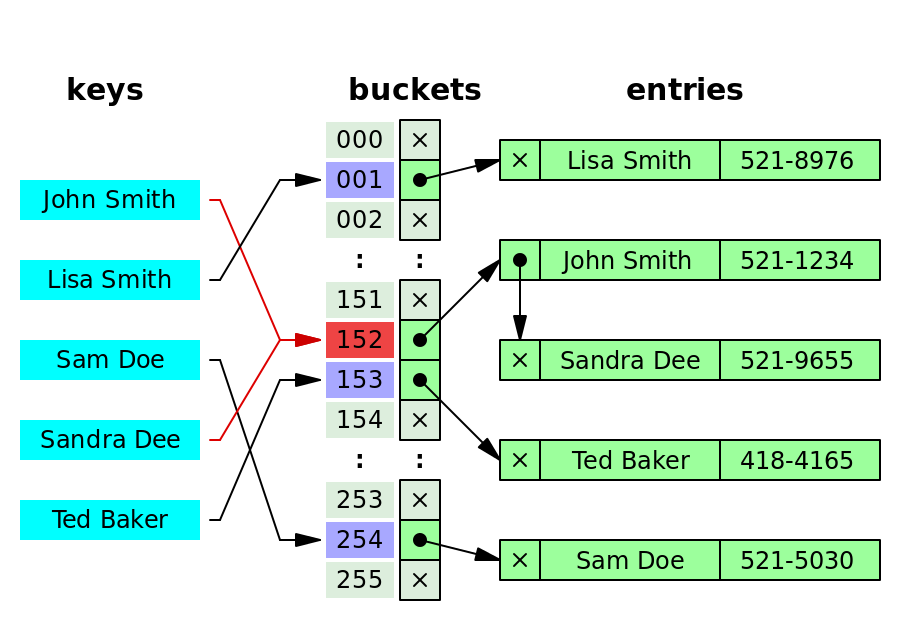
\includegraphics[width=\textwidth]{figures/Wikipedia_hash_table.png}
\vskip1em
\end{column}
\end{columns}

\vspace*{-0.1em}
are the attributes of the primary key, and the \textbf{\alert{values}} are the entire tuples themselves.

\vskip1em
\end{frame}

%
% -------------------------------------------------------------------------------------------------------
%

\begin{frame}

Hash tables are suitable for implementing primary keys and foreign keys efficiently.
\begin{itemize}[-]
\item They provide \emph{Expected} $O(1)$ cost for finding if a key is already in the table, which allows the DBMS to check violations to key constraints.
\end{itemize}

Hash tables are also suitable for implementing joins on primary/foreign key pairs.

\vskip1em

Hashing is also used in a DBMS to implement a set data structure, needed for duplicate elimination.

\end{frame}


%
% -------------------------------------------------------------------------------------------------------
%
\begin{frame}{Static Hashing}

\textbf{Goal}: store and retrieve tuples with \emph{expected} $O(1)$ I/O operations.

Design parameters:
\begin{itemize}[-,noitemsep,topsep=-0.5em]
\item $B$: number of \alert{\emph{buckets}}.
\item \alert{$h()$}: hash function that maps tuples into a number $0 \leq i < B$.
\end{itemize}

 \vskip1em

\begin{columns}[onlytextwidth]
\begin{column}{0.5\textwidth}
Example: $B=4$ buckets.

\vskip1em
- $h(t_1)=2$\\
- $h(t_2)=1$\\
- $h(t_3)=0$\\
- $h(t_4)=1$
\end{column}
\begin{column}{0.5\textwidth}
\setcounter{tIdCnt}{0}
\vskip1em
\scalebox{0.75}{
\begin{tikzpicture}
\staticHashBlock{b0}{0}{0};\node [left= 0.5em of b0] {0};
\staticHashBlock{b1}{0}{-1.5};\node [left= 0.5em of b1] {1};
\staticHashBlock{b2}{0}{-3};\node [left= 0.5em of b2] {2};
\staticHashBlock{b3}{0}{-4.5};\node [left= 0.5em of b3] {3};
\staticHashBlockEntry{b2}{0};
\staticHashBlockEntry{b1}{0};
\staticHashBlockEntry{b0}{0};
\staticHashBlockEntry{b1}{1};
\end{tikzpicture}}
\end{column}
\end{columns}
\end{frame}

%
% -------------------------------------------------------------------------------------------------------
%
\begin{frame}{Good Hash Functions\footnote{\url{https://en.wikipedia.org/wiki/Hash_function}}?}

A \alert{perfect} hash function has the following properties:
\begin{enumerate}[label=(\arabic*)]
\item it is \textbf{fast} to compute

\item it avoids \emph{collisions}: if $t_1 \neq t_2$ then $h(t_1)\neq h(t_2)$

\item it avoids \emph{clustering}: hash values are ``nicely'' spread in $[0, B)$
\end{enumerate}

\vskip1em

A good (and usable) hash function \emph{approximates} these properties.

Typical hash function \framebox{$h(t) = f(t)\mod B$}, where $f(t)$ computes a number out of the tuple (e.g., sum of first 20 bytes in the key).
\end{frame}


%
% -------------------------------------------------------------------------------------------------------
%
\begin{frame}{Insertions with Static Hash Files}

Every new tuple $t_i$ is stored on block $h(t_i)$. 

\vskip1em

If block $h(t_i)$ has room for another tuple, just make the insertion.

\vskip2em

\alert{If $h(t_i)$ is full}, there are two options:
\begin{enumerate}[(1)]
\item Probe subsequent buckets \textbf{sequentially} until an empty slot is found.

\item Grow the buckets with \blue{\emph{overflow} blocks}.
\end{enumerate}

\end{frame}

%
% -------------------------------------------------------------------------------------------------------
%
\begin{frame}

\textbf{Example:} insert new tuple $t_5$ with $h(t_5)=1$

\vskip2em

\begin{columns}[onlytextwidth]
\begin{column}{0.5\textwidth}
Sequential probing:

\vskip1em
\setcounter{tIdCnt}{0}
\scalebox{0.75}{
\begin{tikzpicture}
\staticHashBlock{b0}{0}{0};\node [left= 0.5em of b0] {0};
\staticHashBlock{b1}{0}{-1.5};\node [left= 0.5em of b1] {1};
\staticHashBlock{b2}{0}{-3};\node [left= 0.5em of b2] {2};
\staticHashBlock{b3}{0}{-4.5};\node [left= 0.5em of b3] {3};
\staticHashBlockEntry{b2}{0};
\staticHashBlockEntry{b1}{0};
\staticHashBlockEntry{b0}{0};
\staticHashBlockEntry{b1}{1};
\node [dataBox,yshift = - \dimexpr 0.5pt + (1pt + 1.4em),below right=0.5pt and 0.75pt of b2.north west] {$t_5$};
\draw [->,dotted,thick,color=blue] (b1.east) to [out=315,in=45] ([yshift=-10pt]b2.east);
\end{tikzpicture}}
\end{column}
\begin{column}{0.5\textwidth}
Using overflow blocks:

\vskip1em
\setcounter{tIdCnt}{0}
\scalebox{0.75}{
\begin{tikzpicture}
\staticHashBlock{b0}{0}{0};\node [left= 0.5em of b0] {0};
\staticHashBlock{b1}{0}{-1.5};\node [left= 0.5em of b1] {1};
\staticHashBlock{b2}{0}{-3};\node [left= 0.5em of b2] {2};
\staticHashBlock{b3}{0}{-4.5};\node [left= 0.5em of b3] {3};
\staticHashBlockEntry{b2}{0};
\staticHashBlockEntry{b1}{0};
\staticHashBlockEntry{b0}{0};
\staticHashBlockEntry{b1}{1};

\staticHashBlock{overflow}{3}{-1.5};
\node [dataBox,below right=0.5pt and 0.75pt of overflow.north west] {$t_5$};
\draw [->,thick,color=red] ([yshift=10pt]b1.east) to [out=0,in=180] (overflow);
\end{tikzpicture}}
\end{column}
\end{columns}
\end{frame}

%
% -------------------------------------------------------------------------------------------------------
%
\begin{frame}

\textbf{Sequential probing complicates deletions \textbf{and} searches.}

\vskip2em

\begin{columns}[onlytextwidth]
\begin{column}{0.7\textwidth}
Assume we further insert $t_6$ with $h(t_6) = 2$.

\vskip0.5em

What to do if we wish to \alert{delete} $t_5$?

\vskip2em

\textbf{Option 1:} \emph{compact} the file
\begin{itemize}[-,noitemsep,topsep=-0.5em]
\item Scan the file until the first empty slot after $t_5$.
\item Re-hash all tuples out of place in that interval.
\end{itemize}

\vskip1em

\textbf{Option 2:} put a ``tombstone'' marker (
\includegraphics[height=1em]{figures/RIP.pdf})
\begin{itemize}[-,noitemsep,topsep=-0.5em]
\item \textbf{Ignore tombstones} when \textbf{\alert{searching}}
\item Re-use the spot if possible
\end{itemize}


\end{column}
\begin{column}{0.25\textwidth}
\setcounter{tIdCnt}{0}
\scalebox{0.75}{
\begin{tikzpicture}
\staticHashBlock{b0}{0}{0};\node [left= 0.5em of b0] {0};
\staticHashBlock{b1}{0}{-1.5};\node [left= 0.5em of b1] {1};
\staticHashBlock{b2}{0}{-3};\node [left= 0.5em of b2] {2};
\staticHashBlock{b3}{0}{-4.5};\node [left= 0.5em of b3] {3};
\staticHashBlockEntry{b2}{0};
\staticHashBlockEntry{b1}{0};
\staticHashBlockEntry{b0}{0};
\staticHashBlockEntry{b1}{1};
\node [dataBox,yshift = - \dimexpr 0.5pt + (1pt + 1.4em),below right=0.5pt and 0.75pt of b2.north west] {$t_5$};
\draw [->,dotted,thick,color=blue] (b1.east) to [out=315,in=45] ([yshift=-10pt]b2.east);

\node [dataBox,below right=1pt and 0.75pt of b3.north west] {$t_6$};
\draw [->,dotted,thick,color=magenta] (b2.east) to [out=315,in=45] ([yshift=5pt]b3.east);
\end{tikzpicture}}
\end{column}
\end{columns}
\end{frame}

%
% -------------------------------------------------------------------------------------------------------
%
\begin{frame}

\textbf{Overflow blocks complicate deletions \textbf{and} searches.}

\vskip1em

Assume we further insert $t_5, t_6$ and $t_7$ with $h(t_5) = h(t_6) = h(t_7) = 1$.

\vskip0.5em

What to do if we wish to \alert{delete} $t_5$?

\vskip2em

\begin{columns}[onlytextwidth]
\begin{column}{0.45\textwidth}

\textbf{Option 1:} \emph{compact} the file
\begin{itemize}[-,topsep=-0.5em]
\item May require moving tuples through many blocks
\end{itemize}

\vskip1em

\textbf{Option 2:} leave gaps
\begin{itemize}[-,topsep=-0.5em]
\item Reduces I/O efficiency when searching
\end{itemize}

\end{column}
\begin{column}{0.5\textwidth}
\setcounter{tIdCnt}{0}
\scalebox{0.75}{
\begin{tikzpicture}
\staticHashBlock{b0}{0}{0};\node [left= 0.5em of b0] {0};
\staticHashBlock{b1}{0}{-1.5};\node [left= 0.5em of b1] {1};
\staticHashBlock{b2}{0}{-3};\node [left= 0.5em of b2] {2};
\staticHashBlock{b3}{0}{-4.5};\node [left= 0.5em of b3] {3};
\staticHashBlockEntry{b2}{0};
\staticHashBlockEntry{b1}{0};
\staticHashBlockEntry{b0}{0};
\staticHashBlockEntry{b1}{1};

\staticHashBlock{overflow}{2.75}{-1.5};
\node [dataBox,below right=0.5pt and 0.75pt of overflow.north west] {$t_5$};
\node [dataBox,yshift = - \dimexpr 0.5pt + (1pt + 1.4em),below right=0.5pt and 0.75pt of overflow.north west] {$t_6$};
\draw [->,thick,color=red] ([yshift=10pt]b1.east) to [out=0,in=180] (overflow);

\staticHashBlock{overflow2}{5.5}{-1.5};
\node [dataBox,below right=0.5pt and 0.75pt of overflow2.north west] {$t_7$};
\draw [->,thick,color=red] ([yshift=10pt]overflow.east) to [out=0,in=180] (overflow2);
\end{tikzpicture}}
\end{column}
\end{columns}

\end{frame}

%
% -------------------------------------------------------------------------------------------------------
%
\begin{frame}{I/O cost of Static Hashing}

\textbf{Best case scenario} (one block per bucket and no collisions): the cost of all operations (insertion, search, and deletion) is 1 I/O operation.

\vskip1em

The analysis of the \textbf{average} case cost (with some collisions) gives the same cost for both probing or using overflow chains: $O(\log N)$ for all operations, where $N$ is the number of records in the file.

The same is true for hash file in memory!


\end{frame}

%
% -------------------------------------------------------------------------------------------------------
%
\begin{frame}{Static hashing does not scale}

Static hashing works reasonably well as long as a fraction of blocks that are used remains relatively low (usually, below 75\%).

If the file gets ``too full'' we need to:
\begin{enumerate}[(1),topsep=-0.5em]
\item Add more buckets (increasing $B$)
\item \alert{Re-hash every tuple!} (because $B$ increased!)
\end{enumerate}

\vskip1em

\begin{BOX}{Know your programming language}
In-memory implementations of hash sets and dictionaries/maps in Python and Java use static hashing that grow by \textbf{doubling} in size whenever they are ``too full''.
\end{BOX}


\end{frame}

%
% -------------------------------------------------------------------------------------------------------
%
\begin{frame}{Dynamic Hashing}

Static hashing is bad because growing the hash file is very expensive... requiring to re-hash everything again after certain updates, which can take a very long time.

\vskip2em

\textbf{Dynamic hashing} schemes aim to \alert{grow the hash file incrementally}.

\alert{\textbf{Extensible Hashing}} keeps a dynamic in-memory directory with pointers to disk blocks. (See 11.7 in Silberschatz et al. or 11.3.5 in Garcia-Molina et al.)

\alert{\textbf{Linear Hashing}} grows the hash file one block at a time.

\end{frame}

%
%%!TEX root = ./lec04_access_methods.tex

%
% -------------------------------------------------------------------------------------------------------
%
\begin{frame}{Extensible hashing}

Two ingredients:

\begin{enumerate}[label=(\arabic*)]
\item keep a \textbf{directory} mapping \emph{logical buckets} into physical buckets (i.e., disk blocks)

\item the hash function computes a sequence of $k$ bits (e.g., $k=64$); but only the \alert{first $i$} bits are used to number the logical buckets
\end{enumerate}

\textbf{Example:} $k=4$ and $i=1$

\begin{center}
\setcounter{tIdCnt}{0}
\scalebox{0.75}{
\begin{tikzpicture}
\directory{d}{0}{-1}{1};
\extensibleHashBlock{b0}{2}{0}{1}
\extensibleHashBlock{b1}{2}{-2}{1}
\hashLink{d}{0}{b0}
\hashLink{d}{1}{b1}
\dynamicHashBlockEntry{b0}{0}{0110}{$t_1$}
\dynamicHashBlockEntry{b1}{0}{1011}{$t_2$}
\dynamicHashBlockEntry{b0}{1}{0011}{$t_3$}
\end{tikzpicture}}
\end{center}
\end{frame}


%
% -------------------------------------------------------------------------------------------------------
%
\begin{frame}{Insertion with Extensible Hashing}

Like before, every new tuple $t_i$ goes into bucket $h(t_i)$.

\vskip1em

\textbf{Example:} insert $t_4$ with $h(t_4) = 1001$. 

\vskip1em

\begin{center}
\setcounter{tIdCnt}{0}
\scalebox{0.75}{
\begin{tikzpicture}
\extensibleHashBlock{b0}{2}{0}{1}
\extensibleHashBlock{b1}{2}{-2}{1}
\dynamicHashBlockEntry{b0}{0}{0110}{$t_1$}
\dynamicHashBlockEntry{b1}{0}{1011}{$t_2$}
\dynamicHashBlockEntry{b0}{1}{0011}{$t_3$}


\only<1-2|handout:1>{
	\directory{d}{0}{-1}{1};
	\hashLink{d}{0}{b0}
	\hashLink{d}{1}{b1}
}

\only<2|handout:1>{
	\dynamicHashBlockEntry{b1}{1}{1001}{$t_4$};

	\node (0) at (2.25,-2.8) [thick,color=red,draw,rectangle,minimum height = 1.25em,minimum width = 1.25em] {};
	\node (1) at (-0.45,-1.8) [thick,color=red,draw,rectangle,minimum height = 1.25em,minimum width = 1.25em] {};
	\draw [->,thick, color=red] (0) -- (1);
}
\end{tikzpicture}}
\end{center}
\end{frame}


%
% -------------------------------------------------------------------------------------------------------
%
\begin{frame}

Inserting a tuple into a bucket that is already full forces the \textbf{directory} to grow, by \framebox{increasing \alert{$i$}}.


\vskip1em

\textbf{Example:} insert $t_5$ with $h(t_5) = 0100$. 

\vskip1em

\begin{center}
\setcounter{tIdCnt}{0}
\scalebox{0.75}{
\begin{tikzpicture}
	\extensibleHashBlock{b1}{2}{-4}{1}
	\dynamicHashBlockEntry{b1}{0}{1011}{$t_2$}
	\dynamicHashBlockEntry{b1}{1}{1001}{$t_4$}

\only<1|handout:0>{
	\directory{d}{0}{-1}{1};
	\extensibleHashBlock{b0}{2}{0}{1}	
	\hashLink{d}{0}{b0}
	\hashLink{d}{1}{b1}
	\dynamicHashBlockEntry{b0}{0}{0110}{$t_1$}
	\dynamicHashBlockEntry{b0}{1}{0011}{$t_3$}
}

\only<2-3|handout:1>{
	\directory{d}{0}{-2}{2};
	\extensibleHashBlock{b00}{2}{0}{2}
	\extensibleHashBlock{b01}{2}{-2}{2}

	\hashLink{d}{0}{b00}
	\hashLink{d}{1}{b01}
	\hashLink{d}{2}{b1}
	\hashLink{d}{3}{b1}

	\dynamicHashBlockEntry{b01}{0}{0110}{$t_1$}
	\dynamicHashBlockEntry{b01}{1}{0100}{$t_5$}
	\dynamicHashBlockEntry{b00}{0}{0011}{$t_3$}
}

\only<3|handout:0>{
	\coordinate [left= 1cm of b00] (0) ;
	\draw [->,very thick,color=blue] ([yshift=1em]0) -- ([yshift=5pt]b00.north west);

	\coordinate [left= 1cm of b01] (1) ;
	\draw [->,very thick,color=blue] ([yshift=1em]1) -- ([yshift=5pt]b01.north west);

	\draw [color=red,decorate,decoration={brace,amplitude=5pt,raise=8pt},yshift=0pt]
		(-0.5,-4.2) -- (-0.5,-3) node [midway,xshift=-2.5cm] {
	\begin{minipage}{3.5cm}\baselineskip=0.75\baselineskip \centering
		two logical buckets sharing the same physical bucket
	\end{minipage}
		};
}
\end{tikzpicture}}
\end{center}
\end{frame}


%
% -------------------------------------------------------------------------------------------------------
%
\begin{frame}

\textbf{Example:} insert $t_6$ with $h(t_6) = 0100$. 

\vskip1em

\begin{center}
\setcounter{tIdCnt}{0}
\scalebox{0.75}{
\begin{tikzpicture}
	\extensibleHashBlock{b00}{2}{0}{2}
	\extensibleHashBlock{b1}{2}{-6}{1}
	\dynamicHashBlockEntry{b1}{0}{1011}{$t_2$}
	\dynamicHashBlockEntry{b1}{1}{1001}{$t_4$}
	\dynamicHashBlockEntry{b00}{0}{0011}{$t_3$}

\only<1|handout:0>{
	\directory{d}{0}{-2}{2};

	\extensibleHashBlock{b01}{2}{-2}{2}

	\hashLink{d}{0}{b00}
	\hashLink{d}{1}{b01}
	\hashLink{d}{2}{b1}
	\hashLink{d}{3}{b1}

	\dynamicHashBlockEntry{b01}{0}{0110}{$t_1$}
	\dynamicHashBlockEntry{b01}{1}{0100}{$t_5$}
}

\only<2|handout:1>{
	\directory{d}{0}{-2.5}{3};
	\extensibleHashBlock{b010}{2}{-2}{3}
	\extensibleHashBlock{b011}{2}{-4}{3}

	\hashLink{d}{0}{b00}
	\hashLink{d}{1}{b00}
	\hashLink{d}{2}{b010}
	\hashLink{d}{3}{b011}
	\hashLink{d}{4}{b1}
	\hashLink{d}{5}{b1}
	\hashLink{d}{6}{b1}
	\hashLink{d}{7}{b1}

	\dynamicHashBlockEntry{b011}{0}{0110}{$t_1$}
	\dynamicHashBlockEntry{b010}{0}{0100}{$t_5$}
	\dynamicHashBlockEntry{b010}{1}{0100}{$t_6$}
}
\end{tikzpicture}}
\end{center}
\end{frame}

\newsavebox{\dynamicHashingExample}
\savebox{\dynamicHashingExample}{
\begin{tikzpicture}
	\directory{d}{0}{-2.5}{3};
	\extensibleHashBlock{b010}{2}{-2}{3}
	\extensibleHashBlock{b011}{2}{-4}{3}
	\extensibleHashBlock{b00}{2}{0}{2}
	\extensibleHashBlock{b1}{2}{-6}{1}

	\hashLink{d}{0}{b00}
	\hashLink{d}{1}{b00}
	\hashLink{d}{2}{b010}
	\hashLink{d}{3}{b011}
	\hashLink{d}{4}{b1}
	\hashLink{d}{5}{b1}
	\hashLink{d}{6}{b1}
	\hashLink{d}{7}{b1}

	\dynamicHashBlockEntry{b1}{0}{1011}{$t_2$}
	\dynamicHashBlockEntry{b1}{1}{1001}{$t_4$}
	\dynamicHashBlockEntry{b00}{0}{0011}{$t_3$}
	\dynamicHashBlockEntry{b011}{0}{0110}{$t_1$}
	\dynamicHashBlockEntry{b010}{0}{0100}{$t_5$}
	\dynamicHashBlockEntry{b010}{1}{0100}{$t_6$}
\end{tikzpicture}}

%
% -------------------------------------------------------------------------------------------------------
%
\begin{frame}{Deletions with Extensible Hashing}

Deletions are only an issue if they cause a \textbf{physical} bucket to become empty.

\textbf{Example:} delete tuple $t_1$ with $h(t_1)=0110$.

\vskip1em

\begin{columns}[onlytextwidth]
\begin{column}{0.6\textwidth}
\textbf{Option 1:} \alert{merge logical buckets} (010 and 011 in this case); \alert{shrink the directory} (decrease $i$) if needed\footnotemark.

\vskip1em

\textbf{Option 2:} put a ``tombstone'' mark (
\includegraphics[height=1em]{images/RIP.pdf}) in place of $t_1$. Re-build table when database goes offline for maintenance.
\end{column}
\begin{column}{0.3\textwidth}
\scalebox{0.5}{\usebox\dynamicHashingExample}
\end{column}
\end{columns}
\vskip1em

\footnotetext{Not all deletions lead to shrinking the directory. For example, there would be no shrinking if logical buckets 000 and 001 were on separate physical buckets.}
\end{frame}

%
% -------------------------------------------------------------------------------------------------------
%
\begin{frame}{Too Many Collisions can Break Extensible Hashing}

\textbf{Example:} how to handle the insertion of $t_7$ with $h(t_7)=0100$? 

When more tuples hash to the same bucket than a physical bucket can fit, further growing the directory doesn't help.

\vskip1em

\begin{columns}[onlytextwidth]
\begin{column}{0.6\textwidth}
\textbf{Option 1:} start an \alert{overflow chain} on the block with $t_5$ and $t_6$.

\vskip1em

\textbf{Option 2:} add a level of indirection with ``bucket files''\footnotemark as was done for secondary indexes (slide~\ref{bucket_files_secondary_indexes}). This increases I/O cost.
\end{column}
\begin{column}{0.3\textwidth}
\scalebox{0.5}{\usebox\dynamicHashingExample}
\end{column}
\end{columns}

\footnotetext{Not to be confused with the ``hashing buckets''.}

\end{frame}

%
% -------------------------------------------------------------------------------------------------------
%
\begin{frame}{Extensible Hashing: Summary}

\textbf{Pros:}\\
 - without duplicates, physical buckets are always 1 disk block\\
 - all operations require $O(1)$ I/O (if directory can fit in memory)\\
 - ``file'' on disk grows one block at a time

\textbf{Cons:}\\
 - need to keep directory in memory (or do more I/O)\\
 - directory grows exponentially
 
\vskip1em

\textbf{Worst problem of extensible hashing}: a ``bad'' hash function can cause the directory to grow very big (very fast). Suppose $k=32$ and the number of tuples per bucket is 2 (as in the running example). If there are 3 tuples whose hash values disagree on their $20^{\mathit{th}}$ bit, the directory will grow to $2^{20}$ entries to hold them.
\end{frame}

%
% -------------------------------------------------------------------------------------------------------
% 
%

%
% -------------------------------------------------------------------------------------------------------
%
\begin{frame}{Linear Hashing}

Four ingredients:

\begin{enumerate}[label=(\arabic*)]

\item Distinguish between \emph{virtual} and \emph{materialized} buckets.

\item Use the \alert{last $i$} bits of the hash value as the bucket number.\\[0.5em] If a tuple hashes to a virtual bucket, use the last $i-1$ bits instead (which is guaranteed to map to a materialized bucket).

\item Buckets can span multiple disk blocks (using overflow chains).

\item Add more materialized buckets once the load factor goes over a threshold.
\end{enumerate}
\end{frame}

%
% -------------------------------------------------------------------------------------------------------
%
\begin{frame}

\textbf{Example:} $k=4$ and $i=1$ (meaning, two logical blocks).

\begin{center}

\vskip2em

\scalebox{0.75}{
	\begin{tikzpicture}
	\linearHashVariables{0}{0}{1}{2}{3}
	\linearHashBlock{b0}{3}{0}{0}
	\linearHashBlock{b1}{3}{-1.1}{1}
	\dynamicHashBlockEntry{b0}{0}{0000}{$t_1$}
	\dynamicHashBlockEntry{b0}{1}{1010}{$t_3$}
	\dynamicHashBlockEntry{b1}{0}{1011}{$t_2$}

	\node (0) at (-3,-0.75) [color=red] {
		\begin{minipage}{4cm}\baselineskip=0.75\baselineskip \centering
		number of physical buckets
	\end{minipage}
	};
	\draw[->,color=red,thick] (0) -- (0,-1.15);
	\node (1) at (-2.25,-2.25) [color=blue] {
		\begin{minipage}{2.5cm}\baselineskip=0.75\baselineskip \centering
		number of records in file
	\end{minipage}
	};
	\draw[->,color=blue,thick] (1) -- (0,-2);
	\end{tikzpicture}
}

\vskip3em 

Invariants: \framebox{$i=\ceil{\log_2 n}$} and \framebox{$r/n \leq C \cdot|\text{block}|$}
\end{center}

\vskip1em

$C$ is the \textbf{load factor} above which the file must grow. 

In the example, $|\text{block}|=2$ and the file must grow if $r/n > 1.7$ for a maximum load factor of $C=85\%$.
\end{frame}

%
% -------------------------------------------------------------------------------------------------------
%
\begin{frame}{Finding the bucket of a tuple}
\label{physical_block_in_linear_hashing}

The \alert{\emph{logical} bucket} of tuple $t_i$ is the integer \alert{$m$} corresponding to the \alert{lowest $i$ bits in $h(t_i)$}. 

(1) \alert{$m < n$}: the logical bucket is materialized.\\
 In this case, the \textbf{bucket} of $t_i$ is $m$ itself.

(2) \alert{$m \geq n$}: the logical bucket is virual (i.e., it is not on disk yet).\\
 In this case, the \textbf{bucket} of $t_i$ is the one corresponding to the lowest $i-1$ bits in $h(t_i)$).

\vskip1em

\begin{BOX}{Invariant}
Every tuple has a \textbf{bucket} where it gets stored, even if we do not use all $i$ bits of the hash value.
\end{BOX}
\end{frame}

%
% -------------------------------------------------------------------------------------------------------
%
\begin{frame}{Insertions With Linear Hashing}

\textbf{Algorithm} for inserting tuple $t_i$ into a Linear Hash file

\begin{enumerate}[label=(\arabic*)]
\item determine the \textbf{bucket} of $t_i$ (slide~\ref{physical_block_in_linear_hashing})
\item if the bucket has room, add $t_i$; otherwise, \blue{grow the bucket using an overflow block} and add $t_i$
\item \alert{increase $r$}
\item \alert{if $r/n > C\cdot|\text{block}|$}, add one more bucket to the file and increase $n$ \\[0.5em]\alert{if $\ceil{\log_2 n}>i$}, increase $i$ and \alert{re-hash} the tuples in physical block $n-2^i$
\end{enumerate}
\end{frame}

%
% -------------------------------------------------------------------------------------------------------
%
\begin{frame}

\textbf{Example:} inserting $t_4$ with $h(t_4)=0101$

\vskip2em

\begin{center}
\scalebox{0.75}{
	\begin{tikzpicture}

\only<1|handout:1>{
	\linearHashVariables{0}{0}{1}{2}{3}
}
	\linearHashBlock{b0}{3}{0}{0}
	\linearHashBlock{b1}{3}{-1.1}{1}
	\dynamicHashBlockEntry{b0}{0}{0000}{$t_1$}
	\dynamicHashBlockEntry{b0}{1}{1010}{$t_3$}
	\dynamicHashBlockEntry{b1}{0}{1011}{$t_2$}

\only<2|handout:2>{
	\linearHashVariables{0}{0}{1}{2}{4}
	\dynamicHashBlockEntry{b1}{1}{0101}{$t_4$}

	\node (0) at (-2.5,-1.5) [color=red] {$r/n=2>1.7$};
}
	\end{tikzpicture}
}
\end{center}

\vskip2em

\only<2|handout:2>{
	With the insertion, the load factor is too high and the file needs to grow (next slide).
}
\end{frame}

%
% -------------------------------------------------------------------------------------------------------
%
\begin{frame}{Growing the file; $i$ Increases}
\label{linear_hashing_increase_i}

Adding a bucket makes \alert{$n=3$}; since $\ceil{\log_2 3} > 1$, $i$ is increased, \textbf{doubling} the space of \emph{logical bucket} addresses:
\begin{itemize}[-,noitemsep,topsep=-0.5em]
\item The ``lower half'' of the space has the old buckets
\item The new bucket becomes the \textbf{first} in the ``upper half'': \textcolor{red}{1}$0_{i-1}\cdots 0_0$.
\item We must check for tuples ``out of place'' in \textcolor{red}{0}$0_{i-1}\cdots 0_0$
\end{itemize}

\begin{center}
\vskip1em

\scalebox{0.75}{
	\begin{tikzpicture}

	\linearHashVariables{0}{0}{2}{3}{4}
	\linearHashBlock{b00}{3}{0}{\textcolor{red}{0}0}
	\linearHashBlock{b01}{3}{-1.1}{\textcolor{red}{0}1}
	\linearHashBlock{b10}{3}{-2.2}{\textcolor{red}{1}0}
	\missingLinearHashBlock{b11}{3}{-3.35}{\textcolor{fern}{11}}

	\dynamicHashBlockEntry{b00}{0}{0000}{$t_1$}
	\dynamicHashBlockEntry{b01}{1}{0101}{$t_4$}
	\dynamicHashBlockEntry{b01}{0}{1011}{$t_2$}

\only<1|handout:1>{
	\dynamicHashBlockEntry{b00}{1}{1010}{$t_3$}

	\draw[thick,->,dotted,blue] (b10.east) to [out=15,in=345] (b00.east);

	\node [right=2em of b01,blue] {
		\begin{minipage}{3cm}\baselineskip=0.75\baselineskip \centering \small
		must check for tuples \textbf{ending in 10}
	\end{minipage}
	};
	\node [right of=b11,xshift=-3em,color=fern] {\small not yet added};
}

\only<2|handout:2>{
	\dynamicHashBlockEntry{b10}{0}{1010}{$t_3$}	
	\draw[thick,->,dotted,blue] ([yshift=-5pt]b00.east) to [in=15,out=345] ([yshift=5pt]b10.east);
}
	\end{tikzpicture}}
\end{center}
\end{frame}

%
% -------------------------------------------------------------------------------------------------------
%
\begin{frame}

\begin{block}{Re-hashing tuples out of place}
Whenever we add a new materialized bucket (even when $i$ remains unchanged), we must check for tuples out of place and move them accordingly.
\end{block}

\vskip1em

Let the new materialized bucket be at binary address $\alert{1}\blue{b_{i-1}\cdots b_{0}}$. 

Note that, \underline{prior to adding this block}, any tuple with that exact hash value would have been inserted using less than $i$ bits!

Those tuples would be in the bucket with address $\alert{0}\blue{b_{i-1}\cdots b_{0}}$.

\end{frame}



%
% -------------------------------------------------------------------------------------------------------
%
\begin{frame}
When adding an \alert{overflow} block; $n$ and $i$ stay the same\\

\vskip1em

\textbf{Example:} adding tuple $t_5$ with $h(t_5)=1111$

\begin{center}

\vskip1em

\scalebox{0.75}{
	\begin{tikzpicture}
	\linearHashBlock{b00}{3}{0}{00}
	\linearHashBlock{b01}{3}{-1.1}{01}
	\linearHashBlock{b10}{3}{-2.2}{10}
	\missingLinearHashBlock{b11}{3}{-3.35}{\textcolor{fern}{11}}

	\dynamicHashBlockEntry{b00}{0}{0000}{$t_1$}
	\dynamicHashBlockEntry{b01}{1}{0101}{$t_4$}
	\dynamicHashBlockEntry{b01}{0}{1011}{$t_2$}
	\dynamicHashBlockEntry{b10}{0}{1010}{$t_3$}	

\only<1|handout:1>{
	\linearHashVariables{0}{0}{2}{3}{4}
	\node [right of=b11,xshift=-3em,color=fern] {\small not yet added};
}

\only<2|handout:2>{
	\linearHashVariables{0}{0}{2}{3}{5}
	\linearHashBlock{overflow}{7}{-1.1}{}
	\dynamicHashBlockEntry{overflow}{0}{1111}{$t_5$}

	\draw[->,>=stealth',thick,red] ([yshift=8pt]b01.east) to [out=0,in=180] (overflow);
}
	\end{tikzpicture}}

\vskip1em

\framebox{$n$ \textbf{\alert{does not increase}} when adding an overflow block}

\end{center}
\end{frame}

%
% -------------------------------------------------------------------------------------------------------
%
\begin{frame}

\textbf{Another example} of inserting into empty slots: add tuple $t_6$ with $h(t_6)=0111$

\vskip1em

\begin{center}

\scalebox{0.75}{
	\begin{tikzpicture}

	\linearHashVariables{0}{0}{2}{3}{6}
	\linearHashBlock{b00}{3}{0}{00}
	\linearHashBlock{b01}{3}{-1.1}{01}
	\linearHashBlock{b10}{3}{-2.2}{10}
	\missingLinearHashBlock{b11}{3}{-3.35}{\textcolor{fern}{11}}

	\dynamicHashBlockEntry{b00}{0}{0000}{$t_1$}
	\dynamicHashBlockEntry{b01}{1}{0101}{$t_4$}
	\dynamicHashBlockEntry{b01}{0}{1011}{$t_2$}
	\dynamicHashBlockEntry{b10}{0}{1010}{$t_3$}	

	\linearHashBlock{overflow}{7}{-1.1}{}
	\draw[->,>=stealth',thick,red] ([yshift=8pt]b01.east) to [out=0,in=180] (overflow);
	\dynamicHashBlockEntry{overflow}{0}{1111}{$t_5$}
	\dynamicHashBlockEntry{overflow}{1}{0111}{$t_6$}

	\node (0) at (-2.5,-1.5) [color=red] {$r/n=2>1.7$};

	\end{tikzpicture}}
\end{center}
\vskip2em
With the insertion, the load factor is too high and the file needs to grow (next slide).
\end{frame}

%
% -------------------------------------------------------------------------------------------------------
%
\begin{frame}{Growing the file; $i$ Stays the Same}

\vskip2em

\begin{center}

\scalebox{0.75}{
	\begin{tikzpicture}

\only<1|handout:1>{
	\linearHashVariables{0}{0}{2}{3}{6}
	\dynamicHashBlockEntry{b01}{0}{1011}{$t_2$}
	\dynamicHashBlockEntry{b01}{1}{0101}{$t_4$}
	\linearHashBlock{overflow}{7}{-1.1}{}
	\draw[->,>=stealth',thick,red] ([yshift=8pt]b01.east) to [out=0,in=180] (overflow);
	\dynamicHashBlockEntry{overflow}{0}{1111}{$t_5$}
	\dynamicHashBlockEntry{overflow}{1}{0111}{$t_6$}

	\draw[thick,->,dotted,blue] (b11.east) to [out=15,in=345] (b01.east);
	\node [right=2em of b11,blue] {
		\begin{minipage}{3cm}\baselineskip=0.75\baselineskip \centering \small
		must check for tuples \textbf{ending in 11} (including the overflow block!)
	\end{minipage}
	};

}
	\linearHashBlock{b00}{3}{0}{00}
	\linearHashBlock{b01}{3}{-1.1}{01}
	\linearHashBlock{b10}{3}{-2.2}{10}
	\linearHashBlock{b11}{3}{-3.35}{\textcolor{red}{11}}

	\dynamicHashBlockEntry{b00}{0}{0000}{$t_1$}
	\dynamicHashBlockEntry{b10}{0}{1010}{$t_3$}	

\only<2|handout:2>{
	\linearHashVariables{0}{0}{2}{4}{6}

	\dynamicHashBlockEntry{b01}{0}{0101}{$t_4$}
	\dynamicHashBlockEntry{b11}{0}{1011}{$t_2$}
	\dynamicHashBlockEntry{b11}{1}{1111}{$t_5$}
	
	\linearHashBlock{overflow}{7}{-3.35}{}
	\draw[->,>=stealth',thick,red] ([yshift=8pt]b11.east) to [out=0,in=180] (overflow);

	\dynamicHashBlockEntry{overflow}{0}{0111}{$t_6$}
}
	\end{tikzpicture}}
\end{center}

\vskip2em

\only<2|handout:2>{
With one more insertion we'd have $r=7$ and $r/n>1.7$, forcing the file to grow again ($n$ becomes 5 and $i=\ceil{\log_2 5}=3$, doubling the number of bucket addresses as in Case 1 as in slide~\ref{linear_hashing_increase_i}).
}

\end{frame}

%
% -------------------------------------------------------------------------------------------------------
%
\begin{frame}{Linear Hashing: Summary}

\textbf{Inserting duplicates?} No special treatment... just add the new tuples wherever they hash to.

\textbf{Searching?} Follow steps (1)--(3) of the insertion algorithm (slide~\ref{physical_block_in_linear_hashing}).

\textbf{Deletions?} Just put a ``tombstone'' mark (
\includegraphics[height=1em]{figures/RIP.pdf}) instead of reversing the insertion algorithm.

\vskip1em

\textbf{Access costs?}\\
 - searches, insertions and deletions require, \textbf{in expectation}, at most two I/O operations (1 read and 1 write, if the file grows).

\end{frame}




\section{Multi-key Access Methods}
%!TEX root = ./lec04_access_methods.tex

%
% -------------------------------------
%
\begin{frame}{Multi-Attribute Access}

Goal: finding records satisfying multiple selection criteria at once\\
- \textbf{Ex:} movies where \lstinline[style=cmput391]{year>2010 AND imdb=7.5}.

\vskip1em

\textbf{Option I:} use an index on \alert{either} attribute, and verify the other predicate on the other attribute for each tuple.

\vskip2em

\begin{columns}[onlytextwidth]
\begin{column}{0.5\textwidth}
\scalebox{0.8}{
\begin{tikzpicture}[semithick,align=center,node distance=0.75cm,every node/.style={inner sep=1,outer sep=1,font=\footnotesize}]
\node (0) at (0,0) {} ; %empty node with ``answer''
\node (1) [below of= 0] {$\sigma_{\text{year>2010}}$};
\node (2) [below of= 1] {\lstinline[style=cmput391]{pointer_lookup}};
\node (3) [below of= 2] {\lstinline[style=cmput391]{get_ids(IDX_Movie_imdb, imdb=7.5)}};
\path[->]
    (3) edge (2)
    (2) edge (1)
    (1) edge (0);
\end{tikzpicture}}
\end{column}

\begin{column}{0.5\textwidth}
\scalebox{0.8}{
\begin{tikzpicture}[semithick,align=center,node distance=0.75cm,every node/.style={inner sep=1,outer sep=1,font=\footnotesize}]
\node (0) at (0,0) {} ; %empty node with ``answer''
\node (1) [below of= 0] {$\sigma_{\text{imdb=7.5}}$};
\node (2) [below of= 1] {\lstinline[style=cmput391]{pointer_lookup}};
\node (3) [below of= 2] {\lstinline[style=cmput391]{get_ids(IDX_Movie_year, year>2010)}};
\path[->]
    (3) edge (2)
    (2) edge (1)
    (1) edge (0);
\end{tikzpicture}}
\end{column}
\end{columns}
\end{frame}

%
% -------------------------------------
%
\begin{frame}

\textbf{Option II:} use two indexes, each on a different attribute, and \alert{merge the lists of tuple ids}.

\vskip2em

\begin{center}
\scalebox{0.75}{
\begin{tikzpicture}[semithick,align=center,node distance=1.5cm,every node/.style={inner sep=1,outer sep=1,font=\footnotesize}]
\node (0) at (0,0) {} ; %empty node with ``answer''
\node (3) [below of= 0] {\lstinline[style=cmput391]{intersect_id_lists}};
\node (4) [below left of =3,xshift=-6em] 
	{\lstinline[style=cmput391]{get_ids(IDX_Movie_imdb, imdb=7.5}\lstinline[style=cmput391]{)}};
\node (5) [below right of =3,xshift=6em]
	 {\lstinline[style=cmput391]{get_ids(IDX_Movie_year, year>2010}\lstinline[style=cmput391]{)}};
\path[->]
    (4) edge (3)
    (3) edge (0);
\path[->]
    (5) edge (3);
\end{tikzpicture}}
\end{center}
\end{frame}

%
% -------------------------------------
%
\begin{frame}

\textbf{Option III:}  use a \alert{multidimensional} index. 

As the name suggests, a multidimensional index considers multiple attributes (the dimensions) at the same time. 

Many of them were designed to deal with numeric data, but they can work with all kinds of attributes.

\vskip2em

In the examples that follow, we will consider multidimensional indexes on \lstinline[style=SQL]{(title, year)} keys.

\end{frame}

\newsavebox{\moviesInIMDBYear}
\savebox{\moviesInIMDBYear}{
	\begin{tikzpicture}[
		every node/.style={font=\Large},
	]
	\draw (0,0) rectangle (10,10);
	\coordinate (m1) at (7.8,0.5);\fill (m1) circle [radius=3pt]; \node [above right=3pt and 1pt of m1] {$t_1$};
	\coordinate (m2) at (6.9,1);\fill (m2) circle [radius=3pt]; \node [above right=3pt and 1pt of m2] {$t_2$};
	\coordinate (m3) at (7.8,5.75);\fill (m3) circle [radius=3pt]; \node [above right=3pt and 1pt of m3] {$t_3$};
	\coordinate (m4) at (8.1,8);\fill (m4) circle [radius=3pt]; \node [above right=3pt and 1pt of m4] {$t_4$};
	\coordinate (m5) at (5.3,9);\fill (m5) circle [radius=3pt]; \node [above right=3pt and 1pt of m5] {$t_5$};
	\coordinate (m6) at (1.3,6.8);\fill (m6) circle [radius=3pt]; \node [above right=3pt and 1pt of m6] {$t_6$};
	\coordinate (m7) at (1.9,9.1);\fill (m7) circle [radius=3pt]; \node [above right=3pt and 1pt of m7] {$t_7$};
	\coordinate (m8) at (4,5.2);\fill (m8) circle [radius=3pt]; \node [above right=3pt and 1pt of m8] {$t_8$};
	\coordinate (m9) at (4.25,4);\fill (m9) circle [radius=3pt]; \node [above right=3pt and 1pt of m9] {$t_9$};
	\coordinate (m10) at (1.5,4.25);\fill (m10) circle [radius=3pt]; \node [above right=3pt and 1pt of m10] {$t_{10}$};
	\coordinate (m11) at (8.5,0.25);\fill (m11) circle [radius=3pt]; \node [above right=3pt and 1pt of m11] {$t_{11}$};
	\coordinate (m12) at (9,1.75);\fill (m12) circle [radius=3pt]; \node [above right=3pt and 1pt of m12] {$t_{12}$};
	\end{tikzpicture}
}

\newenvironment{BLOCK}
{\begin{minipage}{20pt}\baselineskip=0.75\baselineskip \centering}
{\end{minipage}}

%
% -------------------------------------
%
\begin{frame}

\textbf{Grid files} are a \emph{hashing-based} representation of multiple points in a $n$-dimensional space.

\vskip1em

Each cell of the grid points to (a chain) of \alert{bucket files}, with pointers to actual tuples (in the data file) that fall in that cell.

\begin{center}
\scalebox{0.4}{
	\begin{tikzpicture}[
		every node/.style={font=\Large},
	]
	\draw (0,0) rectangle (10,10);
	\node at (-0.75,0.125) {\LARGE 1980};
	\node at (-0.75,9.875) {\LARGE 2020};
	\node at (0.125,-0.5) {\LARGE 0};
	\node at (9.875,-0.5) {\LARGE 10};

	\node at (0,0)[anchor=south west,inner sep=0,outer sep=0,xshift=-2.5pt] {\usebox\moviesInIMDBYear};
	\draw [color=red,dashed] (3.33,0) -- (3.33,10);\draw [color=red,dashed] (6.66,0) -- (6.66,10);
	\draw [color=red,dashed] (0,3.33) -- (10,3.33);\draw [color=red,dashed] (0,6.66) -- (10,6.66);

	\node (grid) at (19,5) {
\begin{tikzpicture}[every node/.style={draw,rectangle,minimum width=4em,minimum height=3em}]
	\node (g11) at (0,0) [label=above:0-3.3,label=left:2006-2020] {};
	\node (g12) [right=0pt of g11] [label=above:3.3-6.6] {};
	\node (g13) [right=0pt of g12] [label=above:6.6-10] {};
	\node (g21) [below=0pt of g11] [label=left:1993-2006] {};
	\node (g22) [right=0pt of g21] {};
	\node (g23) [right=0pt of g22] {};
	\node (g31) [below=0pt of g21] [label=left:1980-1993] {};
	\node (g32) [right=0pt of g31] {};
	\node (g33) [right=0pt of g32] {};

	\node (bl11) at (-2,-5)  {\begin{BLOCK}$t_7$\\$t_6$\end{BLOCK}};
	\draw [densely dotted,thick,*->] ([yshift=1.5em]g11.south) -- (bl11);
	\node (bl21) at (-1,-7)  {\begin{BLOCK}$t_{10}$\\~~~\end{BLOCK}};
	\draw [densely dotted,thick,*->] ([yshift=1.5em]g21.south) -- ([xshift=12pt]bl21.north);
	\node (bl12) at (1,-5)  {\begin{BLOCK}$t_5$\end{BLOCK}};
	\draw [densely dotted,thick,*->] ([yshift=1.5em]g12.south) -- (bl12);
	\node (bl22) at (2,-7)  {\begin{BLOCK}$t_8$\\$t_9$\end{BLOCK}};
	\draw [densely dotted,thick,*->] ([yshift=1.5em]g22.south) -- ([xshift=15pt]bl22.north);
	\node (bl13) at (4,-5)  {\begin{BLOCK}$t_4$\end{BLOCK}};
	\draw [densely dotted,thick,*->] ([yshift=1.5em]g13.south) to[out=225,in=90] ([xshift=-5pt]bl13.north);
	\node (bl23) at (5,-7)  {\begin{BLOCK}$t_3$\end{BLOCK}};
	\draw [densely dotted,thick,*->] ([yshift=1.5em]g23.south) to[out=315,in=90] ([xshift=15pt]bl23.north);
	\node (bl33) at (5,-9)  {\begin{BLOCK}$t_1$\\$t_2$\end{BLOCK}};
	\draw [densely dotted,thick,*->,color=blue] ([yshift=1.5em]g33.south) to[out=345,in=0] (bl33.east);
	\node (bl33_b) at (2,-9)  {\begin{BLOCK}$t_{11}$\\$t_{12}$\end{BLOCK}};
	\draw [thick,*->,color=red] ([yshift=-5pt]bl33.north west) to[out=180,in=0] (bl33_b);
\end{tikzpicture}};
	\end{tikzpicture}}
\end{center}
\end{frame}

%
% -------------------------------------
%
\begin{frame}

The boundaries of the grid \alert{need not} be uniformly spaced across dimensions. Moving boundaries to ``balance'' the number of points per grid cell is an interesting optimization problem.

\vskip1em

\begin{center}
\scalebox{0.4}{
	\begin{tikzpicture}[
		every node/.style={font=\Large},
	]
	\draw (0,0) rectangle (10,10);
	\node at (-0.75,0.125) {\LARGE 1980};
	\node at (-0.75,9.875) {\LARGE 2020};
	\node at (0.125,-0.5) {\LARGE 0};
	\node at (9.875,-0.5) {\LARGE 10};

	\node at (0,0)[anchor=south west,inner sep=0,outer sep=0,xshift=-2.5pt] {\usebox\moviesInIMDBYear};
	\draw [color=red,dashed] (3,0) -- (3,10);
	\draw [color=red,dashed] (6.1,0) -- (6.1,10);
	
	\draw [color=red,dashed] (0,4.75) -- (10,4.75);
	\draw [color=red,dashed] (0,0.75) -- (10,0.75);

	\node (grid) at (19,5) {
\begin{tikzpicture}[every node/.style={draw,rectangle,minimum width=4em,minimum height=3em}]
	\node (g11) at (0,0) [label=above:0-3,label=left:1999-2020] {};
	\node (g12) [right=0pt of g11] [label=above:3-6.1] {};
	\node (g13) [right=0pt of g12] [label=above:6.1-10] {};
	\node (g21) [below=0pt of g11] [label=left:1985-1999] {};
	\node (g22) [right=0pt of g21] {};
	\node (g23) [right=0pt of g22] {};
	\node (g31) [below=0pt of g21] [label=left:1980-1985] {};
	\node (g32) [right=0pt of g31] {};
	\node (g33) [right=0pt of g32] {};

	\node (bl11) at (-2,-5)  {\begin{BLOCK}$t_7$\\$t_6$\end{BLOCK}};
	\draw [densely dotted,thick,*->] ([yshift=1.5em]g11.south) -- (bl11);
	\node (bl21) at (-1,-7)  {\begin{BLOCK}$t_{10}$\\~~~\end{BLOCK}};
	\draw [densely dotted,thick,*->] ([yshift=1.5em]g21.south) -- ([xshift=12pt]bl21.north);
	\node (bl12) at (1,-5)  {\begin{BLOCK}$t_5$\\$t_8$\end{BLOCK}};
	\draw [densely dotted,thick,*->] ([yshift=1.5em]g12.south) -- (bl12);
	\node (bl22) at (2,-7)  {\begin{BLOCK}$t_9$\end{BLOCK}};
	\draw [densely dotted,thick,*->] ([yshift=1.5em]g22.south) -- ([xshift=15pt]bl22.north);
	\node (bl13) at (4,-5)  {\begin{BLOCK}$t_4$\\$t_3$\end{BLOCK}};
	\draw [densely dotted,thick,*->] ([yshift=1.5em]g13.south) to[out=225,in=90] ([xshift=-5pt]bl13.north);
	\node (bl23) at (5,-7)  {\begin{BLOCK}$t_2$\\$t_{12}$\end{BLOCK}};
	\draw [densely dotted,thick,*->] ([yshift=1.5em]g23.south) to[out=315,in=90] ([xshift=15pt]bl23.north);
	\node (bl33) at (5,-9)  {\begin{BLOCK}$t_1$\\$t_{11}$\end{BLOCK}};
	\draw [densely dotted,thick,*->] ([yshift=1em]g33.south) to[out=345,in=0] (bl33.east);
\end{tikzpicture}};
	\end{tikzpicture}}
\end{center}
\end{frame}

%
% -------------------------------------
%
\begin{frame}

A \textbf{Quadtree} divides the space into four quadrants, recursively as needed, until each quadrant corresponds to a single block (of a bucket file).\footnote{\url{https://en.wikipedia.org/wiki/Quadtree}}

\begin{center}
\scalebox{0.4}{
	\begin{tikzpicture}[
		every node/.style={font=\Large},
	]
	\draw (0,0) rectangle (10,10);
	\node at (-0.75,0.125) {\LARGE 1980};
	\node at (-0.75,9.875) {\LARGE 2020};
	\node at (0.125,-0.5) {\LARGE 0};
	\node at (9.875,-0.5) {\LARGE 10};

	\node at (0,0)[anchor=south west,inner sep=0,outer sep=0,xshift=-2.5pt] {\usebox\moviesInIMDBYear};
	\draw [very thick,color=red,dashed] (5,0) -- (5,10);\draw [very thick,color=red,dashed] (0,5) -- (10,5);

	%Q1 split
	\draw [color=olive,thick,dashed] (2.5,5) -- (2.5,10);\draw [color=olive,thick,dashed] (0,7.5) -- (5,7.5);
	%Q2 split
	\draw [color=olive,thick,dashed] (7.5,5) -- (7.5,10);\draw [color=olive,thick,dashed] (5,7.5) -- (10,7.5);
	%Q4 split
	\draw [color=olive,thick,dashed] (7.5,0) -- (7.5,5);\draw [color=olive,thick,dashed] (5,2.5) -- (10,2.5);
	%Q4.4 split
	\draw [color=magenta,dashed] (8.75,0) -- (8.75,2.5);\draw [color=magenta,dashed] (7.5,1.25) -- (10,1.25);

	\node (grid) at (19,5) {
\begin{tikzpicture}[
	block/.style={draw,rectangle,minimum width=4em,minimum height=3em},
	tree/.style={thick,draw,ellipse,color=blue},
	direction/.style={fill=background,rectangle,midway}
	]
	\node (root) at (-2,0) [tree] {$5.0, 2000$};

	\node (R_SW) at (-2,-3) [block] {\begin{BLOCK}$t_{10}$\\$t_9$\end{BLOCK}};
	\node (R_NW) at (-5,-3) [tree] {$2.5, 2010$};
	\node (R_NE) at (1,-3) [tree] {$7.5, 2010$};
	\node (R_SE) at (5,-3) [tree] {$7.5, 1990$};
	\draw [->,tree] (root) -- (R_NW) node[direction] {NW};
	\draw [->,tree] (root) -- (R_NE) node[direction] {NE};
	\draw [->,tree] (root) -- (R_SW) node[direction] {SW};
	\draw [->,tree] (root) -- (R_SE) node[direction] {SE};
		
	\node (R_NW_SW) at (-7,-6) [block] {\begin{BLOCK}$t_{6}$\end{BLOCK}};
	\node (R_NW_NW) at (-5.5,-7.5) [block] {\begin{BLOCK}$t_{7}$\end{BLOCK}};
	\node (R_NW_SE) at (-4,-9) [block] {\begin{BLOCK}$t_{8}$\end{BLOCK}};
	\draw [->,tree] (R_NW) -- (R_NW_SW) node[direction] {SW};
	\draw [->,tree] (R_NW) -- (R_NW_NW) node[direction] {NW};
	\draw [->,tree] (R_NW) -- (R_NW_SE) node[direction] {SE};

	\node (R_NE_NW) at (-2,-6) [block] {\begin{BLOCK}$t_{5}$\end{BLOCK}};
	\node (R_NE_NE) at (-0.5,-7.5) [block] {\begin{BLOCK}$t_{4}$\end{BLOCK}};
	\node (R_NE_SE) at (1,-9) [block] {\begin{BLOCK}$t_{3}$\end{BLOCK}};

	\draw [->,tree] (R_NE) -- (R_NE_NW) node[direction] {NW};
	\draw [->,tree] (R_NE) -- (R_NE_NE) node[direction] {NE};
	\draw [->,tree] (R_NE) -- (R_NE_SE) node[direction] {SE};

	\node (R_SE_SE) at (5,-8) [tree] {$8.75, 1985$};
	\node (R_SE_SW) at (3,-6) [block] {\begin{BLOCK}$t_{2}$\end{BLOCK}};
	\draw [->,tree] (R_SE) -- (R_SE_SW) node[direction] {SW};
	\draw [->,tree] (R_SE) -- (R_SE_SE) node[direction] {SE};

	\node (R_SE_SE_SW) at (3,-11) [block] {\begin{BLOCK}$t_1$\\$t_{11}$\end{BLOCK}};
	\node (R_SE_SE_NE) at (4.5,-12.5) [block] {\begin{BLOCK}$t_{12}$\end{BLOCK}};

	\draw [->,tree] (R_SE_SE) -- (R_SE_SE_SW) node[direction] {SW};
	\draw [->,tree] (R_SE_SE) -- (R_SE_SE_NE) node[direction] {NE};
\end{tikzpicture}};
	\end{tikzpicture}}
\end{center}
\end{frame}

%
% -------------------------------------
%
\begin{frame}

All multidimensional indexes extend to more than two dimensions. However, as the number of dimensions grow, so does the complexity of the index \textbf{and} the number of \underline{empty regions} that need to be represented.

The costs of creating and updating these indexes depends on many design decisions of their creators, but in general they required more work than updating unidimensional B+trees or hash files.

\vskip1em

% Like with other indexes, instead of merging/coalescing nodes as the data is updated, most DBMSs periodically re-index the data instead.

One very important multidimensional index (which is covered in the labs), designed for spatial data (e.g., maps), is the ``region tree'' (\alert{\textbf{R tree}}). Like with B+trees, nodes in the R tree correspond to disk blocks and represent (MBRs of) sub-regions of the space, instead of individual points.
\end{frame}





\section{Other Aspects}
%!TEX root = ./lec04_access_methods.tex

%
%
% tuple identifiers
%   --> pointers, virtual memory, database address space
%

\newsavebox\SQLiteRowID
\begin{lrbox}{\SQLiteRowID}\begin{minipage}{0.725\textwidth}
\lstset{style=SQL,%
  keywords=[4]{sqlite},keywordstyle=[4]\ttfamily\bfseries\color{exampleColor},%
  literate =* {>}{{\textcolor{exampleColor}{>}}}1 
              {|}{{{|}}}1} 
\begin{lstlisting}
sqlite> CREATE TABLE Temp(name CHAR(20));
sqlite> INSERT INTO Temp
   ...> VALUES ('Susan'), ('Bob'), ('Susan');
sqlite> SELECT rowid, * FROM Temp;
1|Susan
2|Bob
3|Susan
sqlite>
\end{lstlisting}
\end{minipage}
\end{lrbox}

%
% ---------------------------------------------------------------------------
%
\begin{frame}{Tuple/Row identifiers}

Most DBMSs assign \emph{identifiers} which are unique to every tuple in the same table,\footnote{Sometimes the identifiers are unique within the whole database.} called \emph{tuple} ids or \emph{row} ids.

For example, in SQLite, every tuple is assigned a 64-bit signed integer key that uniquely identifies the tuple in the table--you insert the same data twice, you get two different tuples with different ids.

\vskip1em

\begin{columns}
\begin{column}{0.4125\textwidth}
Tuple ids are typically visible to the application. 

\vskip0.5em

In SQLite, one can even update them.
\end{column}
\begin{column}{0.5\textwidth}
\hspace*{-2em}
\scalebox{0.75}{\fbox{\usebox{\SQLiteRowID}}}
\end{column}
\end{columns}
\end{frame}

\newsavebox\SQLiteDeleteRowID
\begin{lrbox}{\SQLiteDeleteRowID}\begin{minipage}{0.75\textwidth}
\lstset{style=SQL,%
  keywords=[4]{sqlite},keywordstyle=[4]\ttfamily\bfseries\color{exampleColor},%
  literate =* {>}{{\textcolor{exampleColor}{>}}}1 
              {|}{{{|}}}1} 
\begin{lstlisting}
sqlite> DELETE FROM Temp WHERE rowid IN (
   ...>    SELECT rowid FROM Temp t
   ...>    WHERE EXISTS (SELECT t2.rowid
   ...>                  FROM Temp t2
   ...>                  WHERE t2.name=t.name
   ...>                  AND t2.rowid<t.rowid));
sqlite> SELECT rowid, * FROM Temp;
1|Susan
2|Bob
sqlite>
\end{lstlisting}
\end{minipage}
\end{lrbox}

%
% ---------------------------------------------------------------------------
%
\begin{frame}
Tuple ids were initially introduced in relational systems to support the storage of objects in object-oriented programming languages, where object identity is important. Two objects are considered different if their ids are different, regardless of values.

\vskip1em

\begin{columns}
\begin{column}{0.4125\textwidth}
Tuple ids can be useful in some cases, such as eliminating duplicate tuples in relations without keys.
\vskip0.75em

In some DBMSs, tuple ids are actually symbolic references to the record
\end{column}
\begin{column}{0.5\textwidth}
\hspace*{-2em}
\scalebox{0.75}{\fbox{\usebox{\SQLiteDeleteRowID}}}
\end{column}
\end{columns}
for the tuple inside the corresponding data file.

One interesting use of tuple ids is in implementing column stores.
\end{frame}

%
%
% column stores
%
%

%
% ---------------------------------------------------------------------------
%
\begin{frame}{Column-oriented stores}

With a tuple-oriented store (slide~\ref{tuple_oriented_stores}) each record corresponds to an entire tuple of a table. For some applications, this design turns out to be sub-optimal.

In \textbf{scientific applications} it is common for some relations to have hundreds or thousands of attributes, leading to records that are quite large, and a low record/block ratio.

Typical queries in these applications involve only a small fraction of the attributes in the \lstinline[style=SQL]{WHERE} clause and in the value expressions, resulting in a high I/O ``per useful attribute'' cost.

\textbf{On Line Analytical Processing} queries apply over business data often computing aggregations and groupings defined over a small fraction of the schema attributes.

\end{frame}

%
% ---------------------------------------------------------------------------
%
\begin{frame}
The idea behind a column-store is to have separate data files for each of the attributes in the relation. 

For example, the Movie relation in the running example would be stored in four separate data files like so:

\vskip1em

\begin{columns}[onlytextwidth]
\begin{column}[t]{0.3\textwidth}
\scalebox{0.75}{\usebox{\MovieTableColTitle}}
\end{column}
\begin{column}{0.15\textwidth}
\scalebox{0.75}{\usebox{\MovieTableColYear}}
\end{column}
\begin{column}{0.15\textwidth}
\scalebox{0.75}{\usebox{\MovieTableColIMDB}}
\end{column}
\begin{column}{0.3\textwidth}
\scalebox{0.75}{\usebox{\MovieTableColDirector}}
\end{column}
\end{columns}

\vskip1em

This design has some advantages from a storage point of view:\\
 - records are very simple: one id and one attribute;\\
 - \lstinline[style=SQL]{NULL} values are easy to deal with: just ignore them;\\
 - \textbf{data compression} can be used in each file separately.

\end{frame}

%
% ---------------------------------------------------------------------------
%
\begin{frame}
What about query processing?
\vskip1em

\begin{columns}[onlytextwidth]
\begin{column}[t]{0.3\textwidth}
\scalebox{0.75}{\usebox{\MovieTableColTitle}}
\end{column}
\begin{column}{0.15\textwidth}
\scalebox{0.75}{\usebox{\MovieTableColYear}}
\end{column}
\begin{column}{0.15\textwidth}
\scalebox{0.75}{\usebox{\MovieTableColIMDB}}
\end{column}
\begin{column}{0.3\textwidth}
\scalebox{0.75}{\usebox{\MovieTableColDirector}}
\end{column}
\end{columns}

\vskip1em

It is possible to evaluate SQL quite efficiently with column stores. In fact, these systems outperform tuple-stores by quite a margin on most analytical queries.

The main idea is to process each condition in the \lstinline[style=SQL]{WHERE} clause separately, producing a list of tuple ids satisfying each condition. Then merge these lists based on the logical connector: \lstinline[style=SQL]{AND} means intersection, \lstinline[style=SQL]{OR} means union.

Is there anything this design is \textbf{bad} for?\\
 - YES: \lstinline[style=SQL]{SELECT * ...} queries.

\end{frame}

\end{document}